% Options for packages loaded elsewhere
\PassOptionsToPackage{unicode}{hyperref}
\PassOptionsToPackage{hyphens}{url}
\PassOptionsToPackage{dvipsnames,svgnames,x11names}{xcolor}
%
\documentclass[
  11pt,
]{article}
\title{The future is made today: Concerns for reputation foster trust and cooperation}
\author{Thom Benjamin Volker\footnote{I gratefuly acknowledge Davide Barrera, Gary Bolton, Vincent Buskens, Karen Cook, Rense Corten, John Duffy, Vincenz Frey, Elena Katok, Yong-Ju Lee, Nynke van Miltenburg, Axel Ockenfels, Werner Raub, Stephanie Rosenkranz, Arthur Schram, Ingrid Seinen, Joris van der Veer, Jeroen Weesie and Huan Xie for sharing their research data. Also, I wish to thank Vincent Buskens and Werner Raub for their valuable comments and supervision, and Irene Klugkist for stimulating discussions.}}
\date{16 May, 2022}

\usepackage{amsmath,amssymb}
\usepackage{lmodern}
\usepackage{setspace}
\usepackage{iftex}
\ifPDFTeX
  \usepackage[T1]{fontenc}
  \usepackage[utf8]{inputenc}
  \usepackage{textcomp} % provide euro and other symbols
\else % if luatex or xetex
  \usepackage{unicode-math}
  \defaultfontfeatures{Scale=MatchLowercase}
  \defaultfontfeatures[\rmfamily]{Ligatures=TeX,Scale=1}
\fi
% Use upquote if available, for straight quotes in verbatim environments
\IfFileExists{upquote.sty}{\usepackage{upquote}}{}
\IfFileExists{microtype.sty}{% use microtype if available
  \usepackage[]{microtype}
  \UseMicrotypeSet[protrusion]{basicmath} % disable protrusion for tt fonts
}{}
\usepackage{xcolor}
\IfFileExists{xurl.sty}{\usepackage{xurl}}{} % add URL line breaks if available
\IfFileExists{bookmark.sty}{\usepackage{bookmark}}{\usepackage{hyperref}}
\hypersetup{
  pdftitle={The future is made today: Concerns for reputation foster trust and cooperation},
  pdfauthor={Thom Benjamin Volker},
  colorlinks=true,
  linkcolor={blue},
  filecolor={Maroon},
  citecolor={Blue},
  urlcolor={Blue},
  pdfcreator={LaTeX via pandoc}}
\urlstyle{same} % disable monospaced font for URLs
\usepackage[margin=1in]{geometry}
\usepackage{longtable,booktabs,array}
\usepackage{calc} % for calculating minipage widths
% Correct order of tables after \paragraph or \subparagraph
\usepackage{etoolbox}
\makeatletter
\patchcmd\longtable{\par}{\if@noskipsec\mbox{}\fi\par}{}{}
\makeatother
% Allow footnotes in longtable head/foot
\IfFileExists{footnotehyper.sty}{\usepackage{footnotehyper}}{\usepackage{footnote}}
\makesavenoteenv{longtable}
\usepackage{graphicx}
\makeatletter
\def\maxwidth{\ifdim\Gin@nat@width>\linewidth\linewidth\else\Gin@nat@width\fi}
\def\maxheight{\ifdim\Gin@nat@height>\textheight\textheight\else\Gin@nat@height\fi}
\makeatother
% Scale images if necessary, so that they will not overflow the page
% margins by default, and it is still possible to overwrite the defaults
% using explicit options in \includegraphics[width, height, ...]{}
\setkeys{Gin}{width=\maxwidth,height=\maxheight,keepaspectratio}
% Set default figure placement to htbp
\makeatletter
\def\fps@figure{htbp}
\makeatother
\setlength{\emergencystretch}{3em} % prevent overfull lines
\providecommand{\tightlist}{%
  \setlength{\itemsep}{0pt}\setlength{\parskip}{0pt}}
\setcounter{secnumdepth}{5}
\newlength{\cslhangindent}
\setlength{\cslhangindent}{1.5em}
\newlength{\csllabelwidth}
\setlength{\csllabelwidth}{3em}
\newlength{\cslentryspacingunit} % times entry-spacing
\setlength{\cslentryspacingunit}{\parskip}
\newenvironment{CSLReferences}[2] % #1 hanging-ident, #2 entry spacing
 {% don't indent paragraphs
  \setlength{\parindent}{0pt}
  % turn on hanging indent if param 1 is 1
  \ifodd #1
  \let\oldpar\par
  \def\par{\hangindent=\cslhangindent\oldpar}
  \fi
  % set entry spacing
  \setlength{\parskip}{#2\cslentryspacingunit}
 }%
 {}
\usepackage{calc}
\newcommand{\CSLBlock}[1]{#1\hfill\break}
\newcommand{\CSLLeftMargin}[1]{\parbox[t]{\csllabelwidth}{#1}}
\newcommand{\CSLRightInline}[1]{\parbox[t]{\linewidth - \csllabelwidth}{#1}\break}
\newcommand{\CSLIndent}[1]{\hspace{\cslhangindent}#1}
\usepackage{caption,multirow,array,float}
\usepackage{wrapfig}
\usepackage{booktabs}
\usepackage{blkarray}
\usepackage{amsmath}
\usepackage{multicol}
\usepackage{array}
\usepackage{mathtools}
\DeclareCaptionLabelSeparator*{spaced}{\\[2ex]}
\captionsetup[table]{textfont=it,format=plain,justification=justified,
singlelinecheck=false,labelsep=colon,skip=0pt,labelformat=simple}
\usepackage[left]{lineno}
\usepackage{lscape}
% \usepackage[backend=biber]{biblatex}
\usepackage{afterpage}
\usepackage{capt-of}
\newcommand{\blandscape}{\begin{landscape}}
\newcommand{\elandscape}{\end{landscape}}
\newcommand{\bafterpage}{\begin{afterpage}}
\newcommand{\eafterpage}{\end{afterpage}}
\let\oldmaketitle\maketitle
\AtBeginDocument{\let\maketitle\relax}
\usepackage{booktabs}
\usepackage{longtable}
\usepackage{array}
\usepackage{multirow}
\usepackage{wrapfig}
\usepackage{float}
\usepackage{colortbl}
\usepackage{pdflscape}
\usepackage{tabu}
\usepackage{threeparttable}
\usepackage{threeparttablex}
\usepackage[normalem]{ulem}
\usepackage{makecell}
\usepackage{xcolor}
\ifLuaTeX
  \usepackage{selnolig}  % disable illegal ligatures
\fi

\begin{document}
\maketitle


\thispagestyle{empty}
\setstretch{1.5}
\begin{large}
\noindent Research Master's programme 
Sociology and Social Research \newline
Utrecht University, the Netherlands \newline
\newline
\newline
\newline
\newline
MSc Thesis Thom Benjamin Volker (5868777) 
\newline
TITLE: "The future is made today: Concerns for reputation foster trust and cooperation" 
\newline
May 2022 
\newline
\newline
\newline
\newline
\newline
Supervisors:\newline
Prof. Dr. Ir. Vincent Buskens \newline
Prof. Dr. Werner Raub
\newline
\newline
Second grader: \newline
Prof. Dr. Frank van Tubergen
\newline
\newline
\newline
\newline
Preferred journal of publication: Sociological Methods \& Research
\newline
Word count: 23550 (13842 excluding references and appendices; of which 6335 for the data and methods section)
\newline
\addtocounter{page}{-1}
\end{large}
\pagebreak

\let\maketitle\oldmaketitle
\maketitle

\setstretch{2}
\begin{abstract}
When people engage in interactions with a group of common others, they have to consider how their actions today affect their interactions tomorrow.
Even if their future interaction partners differ from those encountered today, information about behavior today might be shared with future partners. 
Although theoretical predictions render trust, and cooperative behavior in general, more likely when today's actions can be sanctioned by others in future interactions, empirical evidence on such effects is inconsistent. 
We investigate the effect of future sanction opportunities through third parties (commonly referred to as the network control effect) by reanalyzing the data from 8 heterogeneous studies using a consistent analysis plan.
Subsequently, we describe and apply a novel method called \textit{Bayesian Evidence Synthesis}, that is applicable regardless of methodological differences between studies, to statistically aggregate the evidence for the network control effect on trustfulness, trustworthiness and cooperation over these studies. 
Our synthesis of results shows that future sanction opportunities by third parties are an effective mechanism to promote trustful, and even more so, trustworthy behavior.
For trustfulness, the evidence is especially convincing when actors can only rely on sanctions by third parties, without being able to apply future sanctions themselves. 
\end{abstract}

\def\fillandplacepagenumber{%
 \par\pagestyle{empty}%
 \vbox to 0pt{\vss}\vfill
 \vbox to 0pt{\baselineskip0pt
   \hbox to\linewidth{\hss}%
   \baselineskip\footskip
   \hbox to\linewidth{%
     \hfil\thepage\hfil}\vss}}

\newpage

\linenumbers

\hypertarget{introduction}{%
\section{Introduction}\label{introduction}}

Smooth social and economic relationships often require trust and cooperation.
In many buyer-seller relationships, for instance, the buyer of a product has to trust that the seller sells high-quality goods, rather than asking high prices for goods of inferior quality.
After all, the buyer may have insufficient knowledge to determine the quality of the good before buying it.
In social exchange (e.g., \protect\hyperlink{ref-blau1964exchange}{Blau 1986}; \protect\hyperlink{ref-Cook2013}{Cook et al. 2013}), someone may help a neighbor, trusting that this neighbor will return the favor in the future.
In both situations, though, at least one of the actors has incentives to exploit the other.
Selling low-quality products for high prices maximizes the returns of the transaction for the seller, while helping a neighbor in return is costly in terms of time and effort but does not yield any additional benefits.
The buyer and the initial helper may anticipate on these incentives to behave opportunistically.
The buyer might refrain from buying the good in the first place, and the initial helper might refrain from helping.
Accordingly, both parties are worse off.
The buyer and the seller do not engage in mutually beneficial exchange, while the neighbors need more time for the tasks they would finish in a trice if they collaborated.
In both examples, goal-directed behavior guided by self-interest impedes coordinating toward a collectively better outcome, characterizing these situations as social dilemmas (\protect\hyperlink{ref-kollock_social_1998}{Kollock 1998}; \protect\hyperlink{ref-ostrom_behavioral_1998}{Ostrom 1998}).

Social dilemmas exemplify how individually rational behavior can lead to unintended and suboptimal consequences for both actors.
The examples, and social dilemma situations in general, can be analyzed in a game-theoretical framework.
This framework helps making assumptions and the derivation of hypotheses explicit, while subsequent tests of the hypotheses allow to revise theoretical arguments by adjusting core assumptions.
From a theoretical perspective, the analysis of dilemma situations allows to map how macro-consequences result from individual behavior.
This can be on the level of two interacting actors, but also on the level of society as a whole, as Hobbes' discussion of the ``problem of order'' (\protect\hyperlink{ref-hobbes_leviathan}{Hobbes {[}1651{]} 1991}) revealed.
According to Hobbes, in a world of scarcity and without external institutions to enforce pro-social behavior, actors may slip into the ``warre of every man against every man,'' although the peaceful alternative would leave everyone better off.
Likewise, opportunistic behavior of individuals may have severe consequences for economic markets, because contractual governance is generally insufficient to cover all possible contingencies that may arise (see \protect\hyperlink{ref-dasgupta_1988}{Dasgupta 1988}; \protect\hyperlink{ref-raub_etal_social_2015}{Raub, Buskens, and Corten 2015} for similar arguments).
`Solving' social dilemma situations can thus improve the efficiency of many social and economic interactions (\protect\hyperlink{ref-buskens_raub_embedded_2002}{Buskens and Raub 2002}; \protect\hyperlink{ref-dasgupta_1988}{Dasgupta 1988}).

Trust and cooperation in social dilemma situations can be fostered by ``embeddedness'' (\protect\hyperlink{ref-granovetter_economic_1985}{Granovetter 1985}).
Everyday interactions are seldom isolated encounters, but rather occur in some social context.
Customers may go to the same store repeatedly or know others who go to this store.
People also have recurring interactions with their neighbors and their neighbors' acquaintances.
Accounting for embeddedness follows from the contributions by \protect\hyperlink{ref-coleman_structure_1986}{Coleman} (\protect\hyperlink{ref-coleman_structure_1986}{1986}) and \protect\hyperlink{ref-granovetter_economic_1985}{Granovetter} (\protect\hyperlink{ref-granovetter_economic_1985}{1985}), who advocated for the specification of robust assumptions on rational individual behavior while allowing for more complexity on the social structure.
Embeddedness operates on two different levels: the dyad level, which refers to the same two actors interacting repeatedly, and the network level, which refers to two actors interacting with common third parties as well (e.g., \protect\hyperlink{ref-buskens_raub_embedded_2002}{Buskens and Raub 2002}, \protect\hyperlink{ref-buskens_raub_handbook_2013}{2013}).
On both levels, embeddedness can foster trustful and trustworthy behavior through \emph{learning} and \emph{control} (\protect\hyperlink{ref-buskens2018trust}{Buskens, Frey, and Raub 2018}; \protect\hyperlink{ref-buskens_raub_embedded_2002}{Buskens and Raub 2002}, \protect\hyperlink{ref-buskens_raub_handbook_2013}{2013}; \protect\hyperlink{ref-yamagishi_yamagishi_trust_1994}{Yamagishi and Yamagishi 1994}).

When people are embedded, they can learn about their partners' past actions through own experiences or through experiences of their acquaintances.
This information may be useful for inferring how a partner will behave in the current interaction, so that one can adapt one's own behavior accordingly.
Obviously, no one wants to buy inferior goods, and neighbors might not help those who broke their promises.
Yet, if you had good experiences with a store, or know that others had good experiences, you may return to go shopping there today, because you expect similar outcomes.
Theoretical and empirical support for such learning effects have been well documented in the sociological and economic literature, both under dyadic (\protect\hyperlink{ref-anderhub_repeated_trust_2002}{Anderhub, Engelmann, and Güth 2002}; \protect\hyperlink{ref-buskens_raub_veer_triads_2010}{Buskens, Raub, and Van der Veer 2010}; \protect\hyperlink{ref-camerer_weigelt_sequential_1988}{Camerer and Weigelt 1988}; \protect\hyperlink{ref-embrey_etal_cooperation_2018}{Embrey, Fréchette, and Yuksel 2018}; \protect\hyperlink{ref-mao_resilient_cooperators_2017}{Mao et al. 2017}; \protect\hyperlink{ref-neral_ochs_sequential_1992}{Neral and Ochs 1992}) and network embeddedness (\protect\hyperlink{ref-bolton_electronic_2004}{Bolton, Katok, and Ockenfels 2004}; \protect\hyperlink{ref-buskens_raub_veer_triads_2010}{Buskens et al. 2010}; \protect\hyperlink{ref-engelmann_firschbacher_2009}{Engelmann and Fischbacher 2009}; \protect\hyperlink{ref-seinen_schram_social_2006}{Seinen and Schram 2006}; \protect\hyperlink{ref-wedekind_milinski_2000}{Wedekind and Milinski 2000}).

The control mechanism refers to one's long-term incentives being under control of future interaction partners (\protect\hyperlink{ref-buskens_raub_embedded_2002}{Buskens and Raub 2002}).
Those who take advantage of others today can be punished in the future, while those who act kindly today can be rewarded, for example with a recurring mutually beneficial exchange relation.
Sanctions, either positive or negative, can be implemented by the person towards whom the sanctioned behavior was directed in the first place.
This is the case of dyadic control.
Network control refers to the possibility to inform others, who can then base their own future behavior on this information.
You may, for instance, return to a seller you had good experiences with, but you could also recommend this seller to others.
In this sense, the future is made today, because someone's behavior today may have lasting consequences that one must consider when deciding how to act.
If there are sufficient control opportunities, that is, if the long-term consequences of a poor reputation may outweigh the short-term gains of opportunistic behavior, it is in one's best interest to build a good reputation today.
Theoretical and empirical findings consistently show positive dyadic control effects on trust and cooperation (\protect\hyperlink{ref-buskens_raub_veer_triads_2010}{Buskens et al. 2010}; \protect\hyperlink{ref-dal_buxf3_cooperation_2005}{Dal Bó 2005}; \protect\hyperlink{ref-dal_buxf3_fruxe9chette_evolution_2011}{Dal Bó and Fréchette 2011}, \protect\hyperlink{ref-dal_buxf3_fruxe9chette_determinants_2018}{2018}; \protect\hyperlink{ref-embrey_etal_cooperation_2018}{Embrey et al. 2018}).
Yet, despite similar \emph{theoretical} results for network control effects (\protect\hyperlink{ref-kandori_social_1992}{Kandori 1992}; \protect\hyperlink{ref-raub_weesie_reputation_1990}{Raub and Weesie 1990}), the \emph{empirical evidence} for network control effects is much more ambiguous (\protect\hyperlink{ref-bolton_electronic_2004}{Bolton et al. 2004}; \protect\hyperlink{ref-buskens_raub_veer_triads_2010}{Buskens et al. 2010}; \protect\hyperlink{ref-corten_etal_reputation_2016}{Corten et al. 2016}; \protect\hyperlink{ref-miltenburg_buskens_triads_2012}{Van Miltenburg, Buskens, and Raub 2012}).

Given such ambiguous evidence, this paper pursues substantive and methodological goals.
The first goal is to assess the empirical evidence concerning network control effects, using data from multiple experimental studies in which games are played in embedded settings in laboratories.
Although all studies assessed effects of network embeddedness, only some examined network control effects specifically.
An even smaller subset found evidence for such effects.
We reanalyze the data from these studies using a consistent analysis plan and statistically summarize the empirical evidence on network control effects.
Moreover, some empirical evidence suggests a difference in network control effects according to the role of an actor.
Some studies found that network control opportunities had an effect on those in the position to exploit their partner (e.g., on the trustworthiness of a seller), but not on those who could be exploited (e.g., on the trustfulness of a buyer; \protect\hyperlink{ref-barrera_buskens_third_2009}{Barrera and Buskens 2009}; \protect\hyperlink{ref-buskens_raub_veer_triads_2010}{Buskens et al. 2010}; \protect\hyperlink{ref-frey_buskens_investments_2019}{Frey, Buskens, and Corten 2019}).
Therefore, the second goal is to explore and quantify to what extent there is more evidence for network control effects on trustworthiness than on trustfulness over all studies.

The third goal of the paper is methodological.
The included studies differ considerably with respect to experimental conditions, such as the specification of the social dilemma, network size, number of transaction partners, and duration of interactions.
Yet, all studies assessed network embeddedness and allow to test for network control effects.
Hence, although not explicitly designed as such, these studies can be considered conceptual replications.
Conceptual replications allow to assess the validity of research findings by investigating whether conclusions hold under alternative conditions, using varying measurement instruments or operationalizations (\protect\hyperlink{ref-nosek_scientific_2012}{Nosek, Spies, and Motyl 2012}).
Previous research has particularly stressed the importance of exact, direct or close replications, which address the statistical reliability of research findings (e.g., \protect\hyperlink{ref-camerer2016evaluating}{Camerer et al. 2016}; \protect\hyperlink{ref-camerer2018evaluating}{Camerer et al. 2018}; \protect\hyperlink{ref-klein_etal_replicability_2014}{Klein et al. 2014}; \protect\hyperlink{ref-nosek_replicability_review_2021}{Nosek et al. 2021}; \protect\hyperlink{ref-open_science_collab_2015}{Open Science Collaboration 2015}).
Conceptual replications add to direct replications by using heterogeneous research designs with different strengths and weaknesses (\protect\hyperlink{ref-lawlor_triangulation_2017}{Lawlor, Tilling, and Davey Smith 2017}; \protect\hyperlink{ref-munafo_robust_2018}{Munafò and Smith 2018}).
A robust line of evidence that allows for greater generalizability is built by combining various ways of testing the same hypotheses, using different sources of data and different methodologies (e.g., \protect\hyperlink{ref-buskens_raub_handbook_2013}{Buskens and Raub 2013}; \protect\hyperlink{ref-jackson_cox_experimental_2013}{Jackson and Cox 2013}; \protect\hyperlink{ref-lawlor_triangulation_2017}{Lawlor et al. 2017}; \protect\hyperlink{ref-munafo_robust_2018}{Munafò and Smith 2018}).
However, such variability complicates the use of conventional approaches for research synthesis, such as meta-analysis (\protect\hyperlink{ref-cooper_handbook_2009}{Cooper, Hedges, and Valentine 2009}; \protect\hyperlink{ref-lipsey_wilson_2001}{Lipsey and Wilson 2001}; \protect\hyperlink{ref-sutton_bayesian_meta2001}{Sutton and Abrams 2001}).
We apply a novel method, called Bayesian Evidence Synthesis (\protect\hyperlink{ref-kuiper_combining_2013}{Kuiper et al. 2013}), which allows to statistically aggregate the evidence over conceptually similar but methodologically diverse studies.

Bayesian Evidence Synthesis (\emph{BES}) builds upon the Bayes Factor (\protect\hyperlink{ref-kass_raftery_bayes_factors_1995}{Kass and Raftery 1995}).
For every study, the support for a hypothesis on the effect of control through network embeddedness can be quantified using a Bayes Factor (\(BF\)).
The study-specific \(BF\)s can subsequently be combined to quantify the overall amount of evidence for the overarching hypothesis that network control fosters trust and cooperation, regardless of the study-specific differences with regard to design and operationalizations of key variables.
Accordingly, \emph{BES} can be used to pool the evidence for a hypothesis over multiple studies, even if the designs differ, and thus enables us to statistically summarize the evidence for a network control effect over our set of studies.
Additionally, \emph{BES} allows to compare the amount of evidence for a network control effect between trustors and trustees.
Rather than pooling effect sizes, \emph{BES} quantifies the evidence over studies in favor of a more general scientific theory by aggregating the relative support for the hypotheses evaluated in each study.
Therefore, besides contributing substantively, we aim to contribute methodologically, by outlining how \emph{BES} can be used to statistically summarize the evidence for a hypothesis over conceptual replications, and how this statistical synthesis of results should be interpreted.

In the upcoming section, we outline the theoretical foundations of network control effects.
Hereafter, we describe the studies that are incorporated in our synthesis, and outline the methodological background of \emph{BES}, including a description of how to apply this method.
In the final sections, we apply \emph{BES} to the data collected in the studies that are considered, and discuss our empirical and methodological findings.

\hypertarget{control-effects-on-trust-the-effect-of-network-control}{%
\section{Control effects on trust: The effect of network control}\label{control-effects-on-trust-the-effect-of-network-control}}

We first introduce the Trust Game as a formal representation of social dilemmas and use it to theorize about control effects.
We restrict ourselves to an informal discussion of control effects, while referring to game-theoretical foundations of our arguments.
With minor modifications, similar theoretical results can be obtained for other dilemma situations that can be represented by different games, such as the Investment Game, Prisoner's Dilemma and Helping Game.
We will not explicitly formulate theoretical arguments for network control effects in these games, but we address the expectations that can be derived from such analyses.

\hypertarget{the-trust-game}{%
\subsection{The Trust Game}\label{the-trust-game}}

The standard one-shot Trust Game in Figure \ref{fig:TG-graph} captures the core elements of previously sketched dilemma situations (e.g., \protect\hyperlink{ref-camerer_weigelt_sequential_1988}{Camerer and Weigelt 1988}; \protect\hyperlink{ref-dasgupta_1988}{Dasgupta 1988}).
The Trust Game involves two actors: actor 1, the ``trustor,'' and actor 2, the ``trustee.''
First, the trustor decides whether to place trust.
If no trust is placed, the game ends and the trustor and trustee receive \(P_i\) (\(i = 1,2\)), respectively.
If trust is placed, the trustee can honor or abuse trust.
Honored trust yields the payoff \(R_i\), which is better for both actors than the situation in which no trust is placed (\(R_i > P_i\)).
Abused trust however yields \(T_2 > R_2\) for the trustee, which shows why the trustee has an incentive to behave untrustworthy.
It is assumed that the actors are completely informed about the structure and the payoffs of the game.
Given that abused trust is associated with payoff \(S_{1} < P_{1} %>
\) for the trustor, anticipating on the trustee's incentives to abuse trust, the trustor is better off by not placing trust in the first place.

\begin{figure}[t]

{\centering 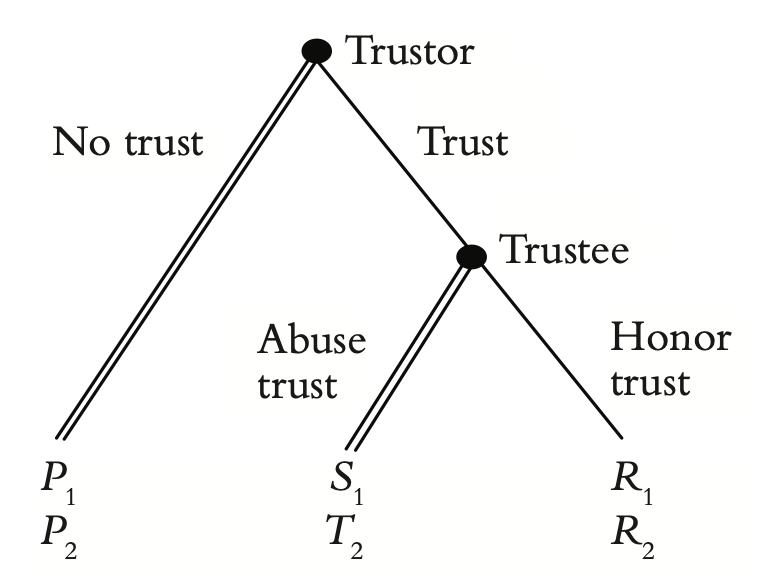
\includegraphics[width=2.59in]{TG} 

}

\caption{Extensive form of a one-shot Trust Game, with $T > R > P > S$. The doubled lines indicate the equilibrium path of play.}\label{fig:TG-graph}
\end{figure}

The Investment Game, Prisoner's Dilemma and Helping Game can be analyzed similarly (e.g., \protect\hyperlink{ref-raub_etal_social_2015}{Raub et al. 2015}).
The Investment Game (\protect\hyperlink{ref-berg_etal_trust_1995}{Berg, Dickhaut, and McCabe 1995}) closely resembles the Trust Game, but differs in one respect: the actors' options are continuous rather than dichotomous.
The trustor obtains an initial endowment, and decides how much of this endowment to send to the trustee.
The experimenter multiplies the amount sent by some factor, after which the trustee decides how much to return to the trustor.
The amounts sent and returned reflect the trustor's trustfulness and the trustee's trustworthiness, respectively.\footnote{
  Note, however, that when a trustor only sends a small amount, the trustee can interpret this as a lack of trust from the trustor.
  If the trustee subsequently returns a small amount, this might be due to (at least) two different reasons: (i) the trustee is opportunistic and returns only little to maximize short-term gains, or (ii) the trustee dislikes not being trusted, and returns little to sanction the trustor for sending a small amount.}
Other dilemma situations may resemble two-sided incentive problems, which can, for instance, be represented by the Prisoner's Dilemma.
In a Prisoner's Dilemma, both actors have incentives to exploit each other, and likewise have an incentive to protect themselves against exploitation by the other.
This contrasts with the Trust Game, which presents the trustee with an incentive to abuse trust, but not the trustor.
The Helping Game resembles the Prisoner's Dilemma, but the actors move sequentially.
Actor 1 decides to help actor 2 at a certain cost that is smaller than the benefit for actor 2, while at a later point actor 2 has the option to help actor 1, irrespective of whether actor 1 helped actor 2 in the first place.

The theoretical analysis of the Trust Game shows that the ``isolated'' nature of the interaction renders trust difficult to achieve, if both actors aim to maximize their individual returns, and the trustor expects the trustee to do so (e.g., \protect\hyperlink{ref-binmore_playing_2007}{Binmore 2007}; \protect\hyperlink{ref-buskens_raub_handbook_2013}{Buskens and Raub 2013}).
The key is that if actors cannot learn about their partner's past actions, and today's actions cannot affect future outcomes, no one has incentives to place or honor trust.
If the actors will not interact in the future, together or with common third parties, there are no control opportunities, because actions cannot be sanctioned.
Hence, nothing withholds a trustee with incentives to abuse trust from acting opportunistically.
Anticipating on the trustee's incentives to abuse trust without adverse future consequences, a trustor may not place trust in the first place out of self-protection.
This renders the outcome of the current interaction suboptimal.
Note that the trustfulness of the trustor predominantly depends on the expected trustworthiness of the trustee (\protect\hyperlink{ref-buskens_raub_embedded_2002}{Buskens and Raub 2002}).
The same reasoning applies to the Investment Game, and similar arguments hold for the Prisoner's Dilemma and the Helping Game.
Although both actors have incentives to behave opportunistically in the latter two games, the point remains that in the absence of future interactions, the short-term gains of exploiting a partner outweigh the future consequences, rendering cooperation unlikely.

\hypertarget{network-control-effects-on-trust}{%
\subsection{Network control effects on trust}\label{network-control-effects-on-trust}}

Taking into account the social context, incentives for the actors may change.
When interactions are embedded, the trustee has to realize that the returns from future interactions are under control of the trustor, and thus has to balance the short-term incentives for abusing trust with the long-term costs.
As said, when the same two partners interact repeatedly, untrustworthy behavior by the trustee today can be retaliated by withholding trust in the future, while trustworthy behavior can be rewarded.
This is often referred to as dyadic control (\protect\hyperlink{ref-buskens_raub_embedded_2002}{Buskens and Raub 2002}), conditional cooperation (\protect\hyperlink{ref-taylor_cooperation_1987}{Taylor 1987}) or direct reciprocity (\protect\hyperlink{ref-nowak_five_2006}{Nowak 2006}; \protect\hyperlink{ref-rand_nowak_cooperation_2013}{Rand and Nowak 2013}). Game-theoretical analyses show that if the costs of future retaliation outweigh the short-term gains of abusing trust, behaving trustworthy is in the trustee's self-interest (\protect\hyperlink{ref-kreps_1990}{Kreps 1990}).\footnote{
  This result holds for both infinitely repeated games with complete information on the incentives of the trustee (e.g., \protect\hyperlink{ref-buskens_raub_handbook_2013}{Buskens and Raub 2013}; \protect\hyperlink{ref-kreps_1990}{Kreps 1990}), as well as for finitely repeated games with incomplete information of the trustor on incentives of the trustee (e.g., \protect\hyperlink{ref-kreps_wilson_reputation_1982}{Kreps and Wilson 1982}).}
Accordingly, the trustor might foresee that an abuse of trust would be against the interests of the trustee, which allows for placing trust (for a more formal discussion, see \protect\hyperlink{ref-buskens2018trust}{Buskens et al. 2018}; \protect\hyperlink{ref-buskens_raub_handbook_2013}{Buskens and Raub 2013}).
Hence, mutually beneficial exchange can follow from actors pursuing their self-interest, such that placing and honoring trust results from equilibrium behavior.
These expectations are well supported in the empirical literature, providing clear evidence for dyadic control effects (\protect\hyperlink{ref-dal_buxf3_cooperation_2005}{Dal Bó 2005}; \protect\hyperlink{ref-dal_buxf3_fruxe9chette_evolution_2011}{Dal Bó and Fréchette 2011}, \protect\hyperlink{ref-dal_buxf3_fruxe9chette_determinants_2018}{2018}; \protect\hyperlink{ref-embrey_etal_cooperation_2018}{Embrey et al. 2018}).

The same mechanism holds when a trustee interacts with several trustors in a network, allowing the trustors to exchange information about the trustee.
If a focal trustor informs future trustors about the trustee's behavior, these future trustors may sanction the trustee for behavior in the focal game.
The long-term payoffs of the trustee are thus still partly under control of the current trustor.
When future trustors sanction the trustee for abusing trust today, the trustee's long-term losses may outweigh the short-term gains from abusing trust, which may mitigate the incentives for abusing trust.
Such network embeddedness can replace (\protect\hyperlink{ref-kandori_social_1992}{Kandori 1992}; \protect\hyperlink{ref-kreps_1990}{Kreps 1990}) or complement (e.g., \protect\hyperlink{ref-buskens_trust_2003}{Buskens 2003}) dyadic embeddedness.
For example, regardless of whether you visit the same seller repeatedly, informing others about your experience with this seller allows them to decide whether they want to interact with this seller.
If enough potential customers avoid the seller based on your information, selling inferior goods will backfire by reducing the seller's future turnover.

If future trustors are reliably informed about the trustee's behavior in the current interaction, they can condition their actions on this behavior (which is often called indirect reciprocity; \protect\hyperlink{ref-nowak_five_2006}{Nowak 2006}; \protect\hyperlink{ref-nowak_sigmund_evolution_2005}{Nowak and Sigmund 2005}).
Accordingly, similar sanctions and rewards can be applied as in dyadically embedded interactions, but potentially by different trustors.
If the potential sanctions are sufficiently severe, it is in the trustee's self-interest to honor trust, and in the trustors self-interest to place trust.
Hence, also under network embeddedness, a mutually beneficial exchange relationship can result from equilibrium behavior.
The severity of the sanctions depends on the likelihood that information about the trustee's past behavior is disseminated, but also on the number of informed future trustors that interact with the focal trustee.
That is, the threat of future sanctions must be credible to have bite.
Accordingly, we expect that trust, and cooperation in general, increases with network control opportunities, leading to the following two hypotheses for the Trust Game and Investment Game:

\begin{itemize}
\tightlist
\item
  Hypothesis \(H_1\): The trustor's trustfulness increases in the amount of network control opportunities.
\item
  Hypothesis \(H_2\): The trustee's trustworthiness increases in the amount of network control opportunities.
\end{itemize}

\noindent
Similar arguments apply to the Prisoner's Dilemma and the Helping Game (e.g., \protect\hyperlink{ref-nowak_sigmund_evolution_2005}{Nowak and Sigmund 2005}; \protect\hyperlink{ref-raub_weesie_reputation_1990}{Raub and Weesie 1990}).
However, these games do not allow to separate trustfulness and trustworthiness.
We therefore restrict the analyses of these studies to a single hypothesis:

\begin{itemize}
\tightlist
\item
  Hypothesis \(H_3\): Cooperation increases in the amount of network control opportunities.
\end{itemize}

Past empirical research obtained inconsistent evidence for these hypotheses.
In the absence of dyadic embeddedness, \protect\hyperlink{ref-bolton_electronic_2004}{Bolton et al.} (\protect\hyperlink{ref-bolton_electronic_2004}{2004}) found support for a network control effect, while \protect\hyperlink{ref-corten_etal_reputation_2016}{Corten et al.} (\protect\hyperlink{ref-corten_etal_reputation_2016}{2016}) did not.
Additionally, multiple studies that did not separate network control effects from other network embeddedness effects found that network embeddedness fostered trust (e.g., \protect\hyperlink{ref-bohnet_learning_2005}{Bohnet et al. 2005}; \protect\hyperlink{ref-bohnet_huck_2004}{Bohnet and Huck 2004}; \protect\hyperlink{ref-duffy2013social}{Duffy, Xie, and Lee 2013}; \protect\hyperlink{ref-huck_competition_2012}{Huck, Lünser, and Tyran 2012}) and cooperation (e.g., \protect\hyperlink{ref-pfeiffer_etal_value_2012}{Pfeiffer et al. 2012}; \protect\hyperlink{ref-seinen_schram_social_2006}{Seinen and Schram 2006}).
When network embeddedness was assessed as an addition to dyadic embeddedness, some support for network control effects was found by \protect\hyperlink{ref-buskens_raub_veer_triads_2010}{Buskens et al.} (\protect\hyperlink{ref-buskens_raub_veer_triads_2010}{2010}), \protect\hyperlink{ref-barrera_buskens_third_2009}{Barrera and Buskens} (\protect\hyperlink{ref-barrera_buskens_third_2009}{2009}) and \protect\hyperlink{ref-frey_buskens_investments_2019}{Frey et al.} (\protect\hyperlink{ref-frey_buskens_investments_2019}{2019}), but not by \protect\hyperlink{ref-miltenburg_buskens_triads_2012}{Van Miltenburg et al.} (\protect\hyperlink{ref-miltenburg_buskens_triads_2012}{2012}).
Although game-theoretical argumentation suggests equivalent dyadic and network control effects, there may be several reasons why the evidence for network control effects is weaker and less consistent than the evidence for dyadic control effects.
First, game-theoretical arguments typically assume that information provided by third parties is reliable, without taking incentive problems with the supply of information into account (\protect\hyperlink{ref-raub_weesie_reputation_1990}{Raub and Weesie 1990}).
Yet, supplying information constitutes a second-order social dilemma, because it takes time and effort to do so, while the individual returns from providing information may be small (\protect\hyperlink{ref-bolton_electronic_2004}{Bolton et al. 2004}).
Additionally, evaluating information from third parties may not be straightforward, especially if the information is inconsistent with own experiences.
Although information is provided consistently and reliably in all experiments considered, participants may attach more value to their own observations.
Lastly, actors may doubt whether others are willing to implement sanctions.
These considerations question the existence of network control effects, for which we aim to quantify the evidence.

\hypertarget{differences-between-network-control-effects-for-trustors-and-trustees}{%
\subsection{Differences between network control effects for trustors and trustees}\label{differences-between-network-control-effects-for-trustors-and-trustees}}

Given that the trustor and the trustee are informed on the structure of the game, and given that they receive the same information before entering an interaction, all network control opportunities are known to both.
Accordingly, game-theoretical predictions render equivalent network control effects for both types of actors.
However, network control opportunities do not need to be evaluated in the same way by both types of actors.
In fact, it may be easier to anticipate on network control opportunities for the trustee than for the trustor (\protect\hyperlink{ref-buskens_raub_veer_triads_2010}{Buskens et al. 2010}).
For trustees, it may be relatively straightforward to anticipate on the fact that abusing trust in a given round will result in repercussions during later rounds.
The reasoning only requires to think one step ahead: if future trustors sanction an abuse of trust, abusing trust will be costly.
If these costs outweigh the gains of abusing trust, it is not worthwhile to act opportunistically.

Before having a good reason to act upon network control opportunities, trustors have to reason one more step ahead.
Specifically, trustors must speculate on how potential future sanctions by other trustors affect a trustee's behavior.
That is, the trustor's trustfulness may increase only if this trustor foresees that the trustee anticipates on how abusing trust now will affect the trustfulness of future trustors, and thus on how future trustors will condition their behavior on the trustee's current actions.
If you do not know whether a seller finds it a credible threat that you inform others after buying inferior goods, the risk of getting exploited might be too high, leading you to refrain from interacting with the seller.
In short, people tend to have difficulties overseeing the complex dynamics of situations with multiple interdependent actors, especially if they have no experience with such situations (\protect\hyperlink{ref-binmore_playing_2007}{Binmore 2007}; \protect\hyperlink{ref-buskens_raub_veer_triads_2010}{Buskens et al. 2010}; \protect\hyperlink{ref-dal_buxf3_cooperation_2005}{Dal Bó 2005}; \protect\hyperlink{ref-dal_buxf3_fruxe9chette_evolution_2011}{Dal Bó and Fréchette 2011}; \protect\hyperlink{ref-milinski_cooperation_2001}{Milinski et al. 2001}). Therefore, we also assess the following conjecture, which can only be assessed for Trust Games and Investment Games:

\begin{itemize}
\tightlist
\item
  Conjecture 1: We expect more evidence for a network control effect on trustees' behavior than on trustors' behavior.
\end{itemize}

\hypertarget{data-and-methods}{%
\section{Data and methods}\label{data-and-methods}}

We assess the evidence for network control effects on trust and cooperation by reanalyzing the data from eight heterogeneous experimental studies (Table \ref{tab:studies-table}).
We attempted to search for and include all experimental studies on network embeddedness effects in two-person dilemma games.
Observational studies were deliberately disregarded, because control and learning effects are typically entangled in real-life settings, rendering the operationalization of the separate constructs without spillover effects extremely challenging.\footnote{In real-life, transaction partners who expect to interact in the future, either with each other or with common third parties, are likely to have interacted in the past, or at least have common acquaintances that provide information on one's partner's past behavior.}
Moreover, we could not obtain the data from 4 of the 13 experimental studies on this topic that we are aware of (\protect\hyperlink{ref-bohnet_learning_2005}{Bohnet et al. 2005}; \protect\hyperlink{ref-bohnet_huck_2004}{Bohnet and Huck 2004}; \protect\hyperlink{ref-huck_competition_2012}{Huck et al. 2012}; \protect\hyperlink{ref-pfeiffer_etal_value_2012}{Pfeiffer et al. 2012}), while we only discovered the existence of one after we finished our study (\protect\hyperlink{ref-duffy_cooperative_2009}{Duffy and Ochs 2009}).
The remaining eight are included.
The studies differed substantially with respect to the game played, game length, operationalization of network embeddedness, network sizes, payoffs and hierarchical structure of the data (see Table \ref{tab:studies-table} and the upcoming section for an elaborate discussion).
Regardless of the conceptual similarities, the variation between studies complicates the use of conventional research synthesis approaches, like meta-analysis.
Yet, Bayesian Evidence Synthesis (\emph{BES}; \protect\hyperlink{ref-kuiper_combining_2013}{Kuiper et al. 2013}) is applicable to quantify the support for the hypotheses over studies.










\afterpage{



\begin{landscape}\begin{table}

\caption{\label{tab:studies-table}Information on all data sets assessed in this study.}
\centering
\resizebox{\linewidth}{!}{
\begin{threeparttable}
\begin{tabular}[t]{>{\raggedright\arraybackslash}p{12.5em}ll>{\raggedright\arraybackslash}p{9em}>{\raggedright\arraybackslash}p{5em}>{\raggedright\arraybackslash}m{9em}l>{\raggedright\arraybackslash}m{10em}}
\toprule
Study & Game & Conditions & Sample size (actions / subjects / sessions) & Actors per network & Number of rounds / continuation probability ($\delta$) & Hypothesis & Multilevel structure (levels)\\
\midrule
\protect\hyperlink{ref-bolton_electronic_2004}{Bolton et al.} (\protect\hyperlink{ref-bolton_electronic_2004}{2004}) & Trust Game & \makecell[l]{1. No embeddedness\\2. Network embeddedness} & 82/82/6 & 16 & 30 rounds & $\beta_{\text{Net}} > \beta_{\text{NoEmb}}$ & Actions (1)\\
 &  &  &  &  &  &  \vphantom{6} & \\
\protect\hyperlink{ref-duffy2013social}{Duffy et al.} (\protect\hyperlink{ref-duffy2013social}{2013}) & Trust Game & \makecell[l]{1. No embeddedness\\2. Network embeddedness with minimal information\\3. Network embeddedness with full information} & 1072/84/14 & 6 & $\delta = 0.8$ & \makecell[l]{$\beta_{\text{NetFull}} > \beta_{\text{NoEmb}}$\\$\beta_{\text{NetMin}} > \beta_{\text{NoEmb}}$} & Actions in individuals in sessions (3)\\
 &  &  &  &  &  &  \vphantom{5} & \\
\protect\hyperlink{ref-seinen_schram_social_2006}{Seinen and Schram} (\protect\hyperlink{ref-seinen_schram_social_2006}{2006}) & Helping Game & \makecell[l]{1. No embeddedness\\2. Network embeddedness} & 52/52/8 & 10/14 & 90 rounds fixed,\newline $\delta = 0.9$ thereafter & $\beta_{\text{Net}} > \beta_{\text{NoEmb}}$ & Actions (1)\\
\addlinespace
 &  &  &  &  &  &  \vphantom{4} & \\
\protect\hyperlink{ref-corten_etal_reputation_2016}{Corten et al.} (\protect\hyperlink{ref-corten_etal_reputation_2016}{2016}) & Prisoner's Dilemma & \makecell[l]{1. No embeddedness\\2. Network embeddedness} & 312/156/19 & 6 & 40 rounds & $\beta_{\text{Net}} > \beta_{\text{NoEmb}}$ & Actions in individuals (2)\\
 &  &  &  &  &  &  \vphantom{3} & \\
\protect\hyperlink{ref-buskens_raub_veer_triads_2010}{Buskens et al.} (\protect\hyperlink{ref-buskens_raub_veer_triads_2010}{2010}) & Trust Game & \makecell[l]{1. Dyadic embeddedness\\2. Dyadic and network embeddedness} & 136/72/4 & 3 & 15 rounds & $\beta_{\text{Net}} > \beta_{\text{Dyad}}$ & Actions in sessions (2)\\
 &  &  &  &  &  &  \vphantom{2} & \\
\addlinespace
\protect\hyperlink{ref-miltenburg_buskens_triads_2012}{Van Miltenburg et al.} (\protect\hyperlink{ref-miltenburg_buskens_triads_2012}{2012}) & Trust Game & \makecell[l]{1. Dyadic embeddedness\\2. Dyadic and network embeddedness} & 522/138/8 & 3 & 15 rounds & $\beta_{\text{Net}} > \beta_{\text{Dyad}}$ & Actions in individuals in sessions (3)\\
 &  &  &  &  &  &  \vphantom{1} & \\
\protect\hyperlink{ref-frey_buskens_investments_2019}{Frey et al.} (\protect\hyperlink{ref-frey_buskens_investments_2019}{2019}) & Trust Game & \makecell[l]{1. Dyadic embeddedness\\2. Dyadic and network embeddedness} & 718/114/6 & 3 & 3 rounds & $\beta_{\text{Net}} > \beta_{\text{Dyad}}$ & Actions in individuals in sessions (3)\\
 &  &  &  &  &  &  & \\
\protect\hyperlink{ref-barrera_buskens_third_2009}{Barrera and Buskens} (\protect\hyperlink{ref-barrera_buskens_third_2009}{2009}) & Investment Game & \makecell[l]{1. Dyadic embeddedness\\2. Dyadic and network embeddedness} & 186/104/6 & 6 & 15 rounds & $\beta_{\text{Net}} > \beta_{\text{Dyad}}$ & Actions in individuals in sessions (3)\\
\bottomrule
\end{tabular}
\begin{tablenotes}[para]
\item \textit{Note.} 
\item The terms $\beta_{\text{Net}}$, $\beta_{\text{NoEmb}}$ and $\beta_{\text{Dyad}}$ in the hypotheses refer to the amount of trustfulness, trustworthiness or cooperation in the condition with network embeddedness (potentially in addition to dyadic embeddedness), in the condition with no embeddedness whatsoever or in the condition with dyadic embeddedness but without network embeddedness. A more elaborate discussion of the exact operationalizations is included in the subsequent section.
\end{tablenotes}
\end{threeparttable}}
\end{table}
\end{landscape}

}

In each study, participants engaged in one or more rounds of a social dilemma game, commonly referred to as a supergame, under varying amounts of network embeddedness.
A supergame is defined as a sequence of identical games, in which information on the behavior of the actors can be transmitted.
Hence, in each supergame, the participants play multiple rounds of the same game.
After each round, information on the outcome of the round is shared with the two actors that interacted in this round.
Dyadic embeddedness implies that the same two actors interact repeatedly, and hence know the outcomes of all previous rounds in which these actors interacted.
Under network embeddedness, the outcome of the interaction of two actors in a given round can be shared with the partners of the actors in one or more subsequent rounds.

We study the network control effect by comparing participants' first-round behavior between embeddedness conditions.
The advantage of focusing on first-round behavior is that participants cannot condition their behavior on past behavior of their partner.
In the first round, either there is no past behavior, because the current interaction takes place in the first, and potentially only, supergame people play.
Alternatively, it can be that participants play multiple supergames, but information about behavior is never shared across supergames.
Hence, focusing on first round behavior allows to separate network control effects from network learning effects.
Given that actors play the same number of rounds in the different embeddedness conditions,\footnote{
  If the supergames had a predetermined endpoint, the number of rounds played in both conditions was exactly equal. If the supergames were terminated randomly with a fixed probability, this probability was the same in both conditions.}
the difference between the embeddedness conditions can solely be ascribed to the difference in sanction opportunities.
Accordingly, in all but one studies we analyze the difference in trustfulness, trustworthiness or cooperation between the embeddedness conditions, without requiring control variables.\footnote{Only in the analysis of the data by \protect\hyperlink{ref-frey_buskens_investments_2019}{Frey et al.} (\protect\hyperlink{ref-frey_buskens_investments_2019}{2019}) a control variable is used, because they employ another experimental manipulation within the varying embeddedness conditions. More detail is provided in the next section.}

In some of the experimental studies considered, the participants played multiple supergames, and hence played multiple ``first rounds.''
In such instances, all ``first rounds'' the participants played were included in the analyses, because playing multiple supergames allows participants to gain experience with the experimental design.
Past research showed that it may take time before participants understand the complex dynamics of social dilemma games, especially in rather artificial experimental settings (e.g., \protect\hyperlink{ref-binmore_playing_2007}{Binmore 2007}; \protect\hyperlink{ref-dal_buxf3_cooperation_2005}{Dal Bó 2005}).
Playing multiple supergames allows participants to gain experience with the experimental set-up.
Note that playing multiple supergames does not allow the participants to ``learn'' in the sense of dyadic or network learning effects, because they do not obtain information about past behavior of their partner.
Nevertheless, participants who play multiple supergames make multiple decisions, which adds to the hierarchical structure of the data.
Such hierarchical nesting is always taken into account (we will discuss this point in more detail when we discuss the analysis models).

Broadly speaking, the data sets can be grouped in two categories.
In the first group, all experiments are characterized by random partner matching.
This implies that participants were randomly matched with a network member before every round of a supergame, and played a single round of a social dilemma game with this partner.
In these experiments, network embeddedness is characterized by the fact that participants obtain information about previous actions of their partner in the current round.
One's behavior in the current round is likewise disseminated to one's partners in future rounds.
The network embeddedness condition was commonly compared with a ``no embeddedness'' condition, in which participants only obtained information about their own interactions.
In the second group of studies, participants played supergames in triads, consisting of two trustors and a single trustee.
Both trustors interact repeatedly with the same trustee, and each participant's role remains constant throughout the supergame.
In contrast to the first set of studies, all trustors are dyadically embedded with the trustee.
Network embeddedness was defined as the presence of a tie between the two trustors, through which information on the trustee's behavior was transmitted.
The ``no embeddedness'' condition is defined as the absence of such a tie.
Hence, the first group generally contrasts a condition with network embeddedness but without dyadic embeddedness with a condition without both forms of embeddedness.
The second group compares a condition with network embeddedness and dyadic embeddedness to a condition with only dyadic embeddedness.
Because of the distinct designs, the results of the studies will be aggregated per set as well.

In the remainder of this section, the characteristics of the included data sets are discussed.
Four design factors of the experimental set-up of each study are described:
\setlength{\parindent}{0in}
\setlength{\leftskip}{0in}
\noindent

\begin{itemize}
  \item{Type of social dilemma game;}
  \item{The interaction network;}
  \item{The number of rounds participants play per supergame;}
  \item{Information provided under the embeddedness conditions.}
\end{itemize}

Additionally, the analysis procedure is discussed in terms of two key features:

\begin{itemize}
  \item{The multilevel structure of the data;}
  \item{The statistical model used (including control variables, if applicable).}
\end{itemize}
\setlength{\parindent}{0.2in}
\setlength{\leftskip}{0in}

A more extensive description of the data, including a discussion of factors that were of interest to the original study, but not to the current, is provided in Appendix \ref{AppA}.
Additional conditions in the original study that impair a clean comparison between a condition with and a condition without network embeddedness are disregarded.\footnote{
  For example, some studies considered the effect of network embeddedness established by the participants themselves, rather than by the experimenter. These conditions are discarded, because the effects of such endogenously chosen forms of embeddedness likely differ from effects of embeddedness imposed by the experimenter.}
Appendix \ref{AppA} also reports on our ability to reproduce the original findings of each study, for those analyses that aligned with the aims of the current study.

\hypertarget{description-of-the-data-sets-considered}{%
\subsection{Description of the data sets considered}\label{description-of-the-data-sets-considered}}

In the upcoming section, the data from each study are discussed. The experiments with random partner matching are described first, followed by the experiments in triads.

\hypertarget{studies-with-random-partner-matching}{%
\subsubsection{Studies with random partner matching}\label{studies-with-random-partner-matching}}

The upcoming four studies all assessed network embeddedness under a random partner matching scheme.
\protect\hyperlink{ref-bolton_electronic_2004}{Bolton et al.} (\protect\hyperlink{ref-bolton_electronic_2004}{2004}) were among the first to study the effect of network embeddedness on trust in the standard Trust Game, using this matching scheme.
All participants played 30 rounds of the Trust Game in a network consisting of sixteen participants.
In the \emph{no embeddedness} condition (consistently denoted \(\beta_{\text{NoEmb}}\) in Table \ref{tab:studies-table}), participants effectively played 30 one-shot Trust Games, in which they were randomly assigned a role (i.e., trustor or trustee) and a partner.
In the \emph{network embeddedness} condition (consistently denoted \(\beta_{\text{Net}}\) in Table \ref{tab:studies-table}), participants were also randomly assigned a role and a partner, but in this condition, the trustors were informed on the total number of times the trustee honored trust in the past and the round-by-round history of past actions.\footnote{The authors also considered a dyadic embeddedness condition, but this condition is disregarded because most studies did not consider dyadic embeddedness separately.}
In both conditions, the participants were always informed on the outcome of their own interactions.
Matches of the same two participants in the same roles were avoided by design.

Because the participants made 30 decisions and were involved in a single group, the actions are nested within individuals, while the individuals are nested within the groups.
However, when only considering first round trustfulness and first round trustworthiness given trustfulness, the nested structure does not apply, as only a single action per subject is considered.
Because participants only interact once with a single partner, it is unlikely that there is any dependence between the actions within a group, because there are no interactions between others that took place before the current interaction.
Hence, the data are analyzed using a regular one-level logistic regression model, in which the outcomes of first round trustfulness (\(0/1\) indicator for placing trust) and trustworthiness (\(0/1\) indicator for honoring trust given that trust is placed) are regressed on network embeddedness (\(0/1\) indicator for the absence/presence of network embeddedness).

Like \protect\hyperlink{ref-bolton_electronic_2004}{Bolton et al.} (\protect\hyperlink{ref-bolton_electronic_2004}{2004}), \protect\hyperlink{ref-duffy2013social}{Duffy et al.} (\protect\hyperlink{ref-duffy2013social}{2013}) assessed the effect of network embeddedness in Trust Games played in networks.
Yet, \protect\hyperlink{ref-duffy2013social}{Duffy et al.} (\protect\hyperlink{ref-duffy2013social}{2013}) implemented a network with six participants (three trustors and three trustees, randomly matched before each round), and the Trust Game was repeated with continuation probability \(\delta = 0.80\), such that the \emph{expected length} of the entire supergame was equal to five rounds.
The roles were assigned to the participants before the start of a supergame.
All rounds within this supergame were played in the same role, but the actors played multiple supergames.
In the ``no embeddedness'' condition, the participants only obtained information on their own history of play, but did not obtain any information about the person they were matched to.
It was thus not possible to infer the behavior of one's partner against oneself in past interactions.
Rather than a single network embeddedness condition, \protect\hyperlink{ref-duffy2013social}{Duffy et al.} (\protect\hyperlink{ref-duffy2013social}{2013}) employed two distinct network embeddedness conditions.
In the ``minimum network embeddedness'' condition (denoted \(\beta_{\text{NetMin}}\) in Table \ref{tab:studies-table}), trustors were informed only on the trustee's behavior in the round prior to the current round.
In the ``full network embeddedness'' condition (denoted \(\beta_{\text{NetFull}}\) in Table \ref{tab:studies-table}), the trustors were informed about the trustee's behavior in up to the 10 most recent periods of the current supergame, and obtained a summary over these rounds.\footnote{\protect\hyperlink{ref-duffy2013social}{Duffy et al.} (\protect\hyperlink{ref-duffy2013social}{2013}) considered two other conditions that are beyond the scope of our study (see Appendix \ref{AppA} or the original study).}
Note that the authors employed a within-subjects design, in which participants played in multiple conditions.
The participants could either play in the ``no embeddedness'' and ``minimum network embeddedness'' condition or in the ``no embeddedness'' and ``full network embeddedness'' condition.

When focusing on first round trustfulness and trustworthiness, part of the multilevel structure can be ignored again.
Yet, since the subjects played multiple supergames with a common group of others, we have to take into account that the actions are nested within individuals, and that the individuals were nested within the group they played with.
We employ logistic regression, with the binary variables trustfulness and trustworthiness (given trustfulness) regressed on embeddedness, and adjust the standard errors for clustering at two levels, which takes the within-subjects design of the data into account.
Additionally, we use separate models for the comparison between no embeddedness (\(0\)) and minimum network embeddedness (\(1\)), and between no embeddedness (\(0\)) and full network embeddedness (\(1\)), because participants exclusively participated in one of the two comparisons.

\protect\hyperlink{ref-seinen_schram_social_2006}{Seinen and Schram} (\protect\hyperlink{ref-seinen_schram_social_2006}{2006}) employed a similar experimental setup, but used another social dilemma game.
In this experiment, the participants played the Helping Game, in which only a single person moves per round.
The subjects played a single supergame in groups of 14, and the supergame lasted at least \(90\) periods.
After the \(90^{th}\) period a continuation probability of \(0.90\) was implemented.
In every round, participants were randomly assigned a role (either donor or recipient) and a partner.
The authors considered the ``no embeddedness'' condition, in which no information on previous choices by the recipient is provided to the donor, and the ``network embeddedness'' condition in which the donors obtained information on up to six previous choices by the recipient, summarized as the number of times the recipient helped and did not help as a donor.\footnote{
  The authors also considered a third condition, similar to the embeddedness condition, but with a different cost of helping than in the other conditions. Due to these different costs, this third condition impairs a fair comparison against the ``no embeddedness'' condition, and hence it is disregarded.}

Like \protect\hyperlink{ref-bolton_electronic_2004}{Bolton et al.} (\protect\hyperlink{ref-bolton_electronic_2004}{2004}), the data has a multilevel structure that can be ignored when only focusing on first round behavior.
Hence, we regress the binary variable ``helping'' on a network embeddedness indicator using a regular logistic regression model.

The study by \protect\hyperlink{ref-corten_etal_reputation_2016}{Corten et al.} (\protect\hyperlink{ref-corten_etal_reputation_2016}{2016}) closely resembles the previous studies, but also differs in important respects.
In \protect\hyperlink{ref-corten_etal_reputation_2016}{Corten et al.} (\protect\hyperlink{ref-corten_etal_reputation_2016}{2016}), participants played a \(2\)-person Prisoner's Dilemma in a network with five others, and all played a single supergame of \(40\) rounds.
In every round, each participant was randomly matched to two others, and played the game with both of these separately.
After each round, each participant was informed on the outcome of both interactions.
The authors compared a ``no embeddedness'' condition, in which participants only obtained information on the outcome of their own interactions, with a ``network embeddedness'' condition, in which participants were informed on the outcome of all interactions in each round.
Unlike the previous studies, participants were informed on the identity of their partners.
The combination of the identifiability of past partners and a game length of 40 rounds with two partners per round in groups of \(6\) (which yields expectedly \(16\) interactions between each pair of actors), renders a substantial amount of dyadic embeddedness in both conditions.
Hence, rather than combining ``no embeddedness with''network embeddedness'', the comparison is closer to ``dyadic embeddedness'' versus ``network embeddedness and dyadic embeddedness.''

The corresponding data has a nested structure, that cannot be ignored, because each participant makes two simultaneous decisions in the first round.
We therefore apply a logistic regression model in which cooperation is regressed on network embeddedness, with cluster-adjusted standard errors on the level of the individual.

\hypertarget{studies-in-triads}{%
\subsubsection{Studies in triads}\label{studies-in-triads}}

We now describe the studies on games played in triads.
\protect\hyperlink{ref-buskens_raub_veer_triads_2010}{Buskens et al.} (\protect\hyperlink{ref-buskens_raub_veer_triads_2010}{2010}) conducted an experiment on behavior in Repeated Triad Trust Games, which was replicated in \protect\hyperlink{ref-miltenburg_buskens_triads_2012}{Van Miltenburg et al.} (\protect\hyperlink{ref-miltenburg_buskens_triads_2012}{2012}).
In both studies, participants played fifteen rounds of the Trust Game within a triad that was formed before the start of the first round, consisting of two trustors and one trustee.
In every round, the first trustor interacts first with the trustee, after which the second trustor interacts with the same trustee.
In both studies, two conditions were considered.
In the ``no network embeddedness'' condition (consistently denoted \(\beta_{\text{Dyad}}\) in Table \ref{tab:studies-table}), the trustors were immediately informed about the outcomes of their own interactions with the trustee, such that the trustor and trustee were dyadically embedded.
In the ``network embeddedness'' condition, the trustors were informed about the outcomes of their own interactions, but also received information on the outcomes of the interactions between the other trustor and trustee.
Accordingly, the trustors could act upon own experiences, and upon experiences by the other trustor, representing a situation with both dyadic and network embeddedness.

In the study by \protect\hyperlink{ref-buskens_raub_veer_triads_2010}{Buskens et al.} (\protect\hyperlink{ref-buskens_raub_veer_triads_2010}{2010}), the participants played once in every role, resulting in a complicated cross-classified nesting structure: actions are nested in supergames and in individuals, and individuals play multiple supergames in different triads.
However, this structure can be mostly ignored when focusing on first round behavior of, and towards, the first acting trustor.
In each supergame, the first interaction between the first acting trustor and the trustee are assessed, because these are the only actions that are free of potential learning effects, resulting in one action per participant, with participants nested within sessions.
Because adjusting the standard errors for clustering at the session level yields an estimated cluster-adjusted standard error that equals zero, we analyze the data with a logistic regression model with unadjusted standard errors, in which trustfulness and trustworthiness are regressed on the embeddedness condition.

In the study by \protect\hyperlink{ref-miltenburg_buskens_triads_2012}{Van Miltenburg et al.} (\protect\hyperlink{ref-miltenburg_buskens_triads_2012}{2012}) the subjects played twice in every role.
Focusing on first-round interactions between the first trustor and the trustee yields multiple actions per participant, with participants nested within the sessions.
Accordingly, we fit a logistic regression model with cluster-adjusted standard errors, in which the binary variables trustfulness and trustworthiness are regressed on the embeddedness condition.

\protect\hyperlink{ref-frey_buskens_investments_2019}{Frey et al.} (\protect\hyperlink{ref-frey_buskens_investments_2019}{2019}) built upon the previous Repeated Triad Trust Game studies, but somewhat altered the specifications of the game.
First, each trustor plays three, rather than 15 rounds.
Additionally, the authors introduced incomplete information, in the sense that the trustors do not know whether the trustee has incentives to abuse trust.
When a trustee has no incentive to abuse trust, the trustee's payoff for abusing trust is altered by the experimenter, such that abusing trust yields the lowest payoff.
While the trustees know whether they have incentives to abuse trust before the interaction starts, the trustors do not have this information.
The trustors only know the probability that the incentives of the trustee are altered (see Appendix \ref{AppA} for more information).
Incomplete information was implemented in all conditions, such that our expectations on the effects of embeddedness are unlikely to be affected.
These authors also consider two embeddedness conditions.
In the ``no network embeddedness'' condition, the trustors only obtain information about the outcomes of their own interactions with the trustee, and in the ``network embeddedness'' condition, the trustors obtain information about both their own and the other's outcome.\footnote{\protect\hyperlink{ref-frey_buskens_investments_2019}{Frey et al.} (\protect\hyperlink{ref-frey_buskens_investments_2019}{2019}) also consider two conditions in which the actors could choose to invest in network embeddedness. However, these conditions are disregarded, because authors who are willing to invest in embeddedness might have an advanced understanding of the game, might be more willing to act trustful and trustworthy because they invested (i.e., the sunk cost fallacy), or might in other ways differ from those who do not invest in network embeddedness, which can affect the results of the analysis.}
Additionally, the authors introduce three incomplete information conditions, all with a different probability to encounter a trustee without incentives to abuse trust (this probability equals \(0.05\), \(0.20\) or \(0.40\)).
Although this experimental manipulation is not of substantive interest, it will be statistically controlled for.

The authors employed a within-subjects design, in which the subjects played in both embeddedness conditions.
Additionally, each subject played 12 supergames, four times in each role. Hence, the nesting structure is cross-classified, with every action nested within an individual, while individuals play multiple supergames, all within an experimental session.
When focusing on first round behavior of and against the first acting trustor, we can ignore the nesting in supergames, and thus consider actions, nested in individuals, nested in sessions.
The data is analyzed using logistic regression with cluster-adjusted standard errors, in which trustfulness and trustworthiness are regressed on the embeddedness indicator, controlling for the different probabilities of encountering a trustee without incentives to abuse trust (included in the analyses as dummy variables; the estimated coefficients for these dummies are reported in Appendix \ref{AppB}).
Note that trustworthiness is only assessed for trustees with an incentive to abuse trust.

In contrast to the previous three studies, \protect\hyperlink{ref-barrera_buskens_third_2009}{Barrera and Buskens} (\protect\hyperlink{ref-barrera_buskens_third_2009}{2009}) assess embeddedness effects using Investment Games.
The Investment Game was played in networks of six actors, with four trustors and two trustees.
Two of the trustors both interact for 15 rounds with one of the trustees, and the other two trustors have 15 interactions with the other trustee.
Unlike the previous triad studies, the trustors interact simultaneously with the trustee, rather than sequentially.
The authors consider two embeddedness conditions.
In the ``network embeddedness'' condition, the trustors obtain information from the outcomes of interactions (i.e., the amounts sent and returned) between the other trustor playing with the same trustee after each round.
Hence, misdemeanors against one of the trustors can be sanctioned by both.
In the ``no network embeddedness'' condition, the trustors receive information on another trustor, playing with \emph{another} trustee.
Although there is some information dissemination through the network, this information does not allow for sanctions, and hence the term ``no network embeddedness.''
All subjects first played in the network embeddedness condition, and thereafter in the no network embeddedness condition, and played both conditions in the same role.
The authors vary multiple other factors that are not of interest in the current study (see Appendix \ref{AppA} or \protect\hyperlink{ref-barrera_buskens_third_2009}{Barrera and Buskens} (\protect\hyperlink{ref-barrera_buskens_third_2009}{2009}) for a full description).

The data has a nested structure, with actions nested in supergames and in individuals, both nested in sessions.
When focusing on first round behavior, the level of the supergames can be ignored for the trustors.
Because the trustors act simultaneously, and the trustee has to decide how to respond to both at the same time, each trustee makes two decisions in the first round.
Theoretically, a linear regression model with cluster-adjusted standard errors on the level of the individual and the level of the session can be applied for the trustors.
However, as taking the clustering into account reduces, rather than increases, the standard error of the regression coefficients, we opt for the most conservative choice, and fit a linear regression model with conventional standard errors, in which trustfulness (the proportion of the initial endowment sent to the trustee) is regressed on network embeddedness.
For the trustees, a linear regression model with cluster-adjusted standard errors on the level of the supergame, the individual and the session should be fitted.
Again, incorporating the level of the supergame drastically decreases the standard error of the coefficient.
Hence, we fit a linear regression model with cluster-adjusted standard errors on the level of the individual and the session, in which trustworthiness (the proportion of the amount sent that is returned to the trustor) is regressed on the embeddedness condition.

\hypertarget{bayesian-evidence-synthesis}{%
\subsection{Bayesian Evidence Synthesis}\label{bayesian-evidence-synthesis}}

Despite the conceptual similarities between the aforementioned studies, the methodological differences render conventional approaches for research synthesis, such as meta-analysis, unfeasible (\protect\hyperlink{ref-cooper_handbook_2009}{Cooper et al. 2009}; \protect\hyperlink{ref-lipsey_wilson_2001}{Lipsey and Wilson 2001}).
The heterogeneity between studies results in multiple embeddedness effects for which the effect sizes are not directly comparable, due to the use of different games, different specifications of the conditions and different statistical models.
Hence, combining the parameter estimates of a network control effect into a single ``pooled'' effect is not straightforward.
\emph{BES} allows to combine the support for a scientific theory or an overall hypothesis, by shifting the focus from parameter estimation to hypothesis evaluation.
Unlike meta-analysis, \emph{BES} does not allow to estimate an ``aggregated'' effect-size, which might be regarded as a shortcoming of the approach.
Obtaining effect sizes is generally desirably, and important to determine whether estimated effects are also statistically relevant.
Yet, in the context of heterogeneous studies, obtaining an aggregate effect size might not be too informative, as the effect size is likely to differ according to the experimental set-up and the contrasted conditions.
That is, the aggregated effect size might not be easy to interpret, or even become meaningless due to different scales.

Using \emph{BES}, we build upon the work by \protect\hyperlink{ref-kuiper_combining_2013}{Kuiper et al.} (\protect\hyperlink{ref-kuiper_combining_2013}{2013}), who developed the methodology and applied it on four studies that assessed dyadic learning effects.
While methodologically insightful, their empirical results were less surprising, as all studies considered consistently found support for the hypothesis under consideration.
In the present paper, we apply \emph{BES} to multiple studies, of which those that already assessed network control effects found inconsistent results.
Hence, we use \emph{BES} to answer substantive research questions that could not have been answered before.
In every study, the network control hypotheses will be formalized as informative hypotheses.
Accordingly, Bayesian evaluation of informative hypotheses will be applied on the level of the individual studies, and the resulting support for the hypotheses will be aggregated using \emph{BES}.
That is, we apply \emph{BES} to statistically aggregate the support for the network control hypotheses, regardless of the differences between the studies.
Simultaneously, we extend the work by \protect\hyperlink{ref-kuiper_combining_2013}{Kuiper et al.} (\protect\hyperlink{ref-kuiper_combining_2013}{2013}) by discussing the methodological consequences of different alternative hypotheses (that is, the hypotheses with which the network control hypotheses are contrasted).
In the remainder of this section, we discuss each ingredient of \emph{BES}: informative hypotheses, Bayesian evaluation of informative hypotheses, and the aggregation procedure of \emph{BES}.

\hypertarget{informative-hypotheses}{%
\subsubsection{Informative hypotheses}\label{informative-hypotheses}}

In the conventional framework of null-hypothesis testing, the classical null hypothesis implies that the hypothesized relationship is non-existent (e.g., the network control effect equals zero).
The null hypothesis is generally evaluated against the traditional alternative hypothesis, indicating that the hypothesized relationship can be anything (e.g., the network control effect differs from zero, leaving implicit how this effect differs from zero).
That is, the alternative hypothesis is often an unconstrained hypothesis, in the sense that no constraints are placed on the estimated parameters of the model, such that they can take any value.
A scientific theory or theoretical hypothesis can also be formalized as an informative hypothesis (\protect\hyperlink{ref-hoijtink_informative_2012}{Hoijtink 2012}; \protect\hyperlink{ref-klugkist_volker}{Klugkist and Volker n.d.}).
Evaluation of informative hypotheses is a statistical technique that allows researchers to evaluate their expectations more directly than through null hypothesis testing.
When researchers evaluate a one-sided hypothesis (e.g., a one-sided \(t\)-test), they, in fact, evaluate an informative hypothesis.
As such, informative hypotheses allow to explicitly formalize the researchers' expectations on the parameters of the statistical model (\protect\hyperlink{ref-hoijtink_klugkist_boelen_2008}{Hoijtink, Klugkist, and Boelen 2008}).
Informative hypotheses can be relatively simple, such as in the case of a one-sided hypothesis test, but can also become rather complex, with simultaneous expectations on multiple parameters (e.g., all regression coefficients in a model are positive).
In the context of the current study, we expect a positive network control effect, in the sense that there is more first round trust and cooperation in conditions with network embeddedness.
Capturing this expectation in informative hypotheses yields
\[
\begin{matrix*}[l]
H_1: & \beta_{\text{Net-tf}} & > & 0, \\
H_2: & \beta_{\text{Net-tw}} & > & 0, \\
H_3: & \beta_{\text{Net-coop}} & > & 0,
\end{matrix*}
\]
stating that there is a positive effect of network embeddedness on trustfulness, trustworthiness and cooperation, respectively.
These hypotheses are equivalent to the hypotheses specified in Table \ref{tab:studies-table}, given that the conditions without network embeddedness are considered as the reference categories.
We contrast the hypotheses with the alternative hypotheses that the hypothesized relationships are \emph{not} true.
That is, these hypotheses are compared with their respective complements, indicating that the effects are smaller than or equal to zero.
Additionally, we compare the hypotheses of interest with an unconstrained alternative hypothesis.
Although the unconstrained hypothesis is of little substantive interest, as it allows the parameters to take on \emph{any} value, it renders a more conservative evaluation of our hypotheses.
We return to these considerations in the subsequent section, and when discussing the results of our analyses.

Informative hypotheses can be evaluated using a Bayesian approach.
Whereas the conventional significance testing approach only allows to reject the null hypothesis (i.e., it is formally impossible to accept the null hypothesis), Bayesian evaluation allows to quantify the support for all hypotheses under consideration.
This framework is more in line with the idea that statistical inference should not be focused on rejecting a null hypothesis (e.g., \protect\hyperlink{ref-cohen_earth_1994}{Cohen 1994}; \protect\hyperlink{ref-lykken_wrong_1991}{Lykken 1991}), but rather on comparing scientifically meaningful hypotheses (\protect\hyperlink{ref-royall1997statistical}{Royall 1997}).
Even if researchers specify scientifically meaningful hypotheses, and evaluate these through one-sided hypothesis tests, the classical hypothesis test and resulting \(p\)-value cannot provide the support for either of the two hypotheses.
Bayesian evaluation of informative hypotheses allows to make a meaningful comparison between hypotheses, by expressing the support in the data for each of the hypotheses under consideration.

\hypertarget{bayesian-evaluation-of-informative-hypotheses}{%
\subsubsection{Bayesian evaluation of informative hypotheses}\label{bayesian-evaluation-of-informative-hypotheses}}

The hypotheses must be evaluated in each study separately.
Within the Bayesian framework, the models used to analyze the data are combined with a prior distribution on the parameters of the model, resulting in the posterior distribution of the parameters given the data and the hypotheses.
The aforementioned statistical models used to analyze the data from the experiments fall under the generalized linear model (GLM) family.
GLMs use some link function \(g(\cdot)\) to transform the linear predictor \(\eta = X\beta\) (\(X\) denotes the matrix containing the predictor variables, while \(\beta\) denotes the vector with regression coefficients) into the predicted value on the outcome variable \(Y\) for all observations.
The likelihood of the parameters given the data under the generalized linear model is formalized as
\[
L(\beta, \phi | Y, X) \equiv f(Y|X, \beta, \phi) = \prod^n_{i=1} f(Y_i | X_i, \beta, \phi),
\]
where \(i\) is an indicator for each individual observation and \(\phi\) denotes the variance or dispersion parameter.

In most studies, the outcome variable is dichotomous (i.e., actors trust/cooperate or they do not), which renders the logistic regression model applicable.
The corresponding likelihood is defined by
\[
L(\beta | Y, X) = \prod^n_{i=1} p_i^{Y_i} (1 - p_i)^{1 - Y_i},
\]
where \(Y_i\) is either \(0\) or \(1\), \(p_i = \frac{1}{1 + \text{exp}\{-X_i\beta\}}\) and the dispersion parameter is omitted because it is fixed at \(\phi = 1\).
The data collected by \protect\hyperlink{ref-barrera_buskens_third_2009}{Barrera and Buskens} (\protect\hyperlink{ref-barrera_buskens_third_2009}{2009}) is analyzed with a linear regression model, which yields the likelihood
\[
L(\beta, \sigma^2 | Y, X) = \prod^n_{i=1} \frac{1}{\sqrt{2\pi\sigma^2}} \text{exp}\Bigg\{-\frac{(Y_i - X_i\beta)^2}{2\sigma^2}\Bigg\},
\]
in which the dispersion parameter is represented by the more common notation \(\sigma^2\).

After defining the analysis model, the prior distribution for the parameters in the model must be specified to obtain the posterior distribution.
Because the prior and posterior distribution under an unconstrained hypothesis encompass the prior and posterior under constrained hypotheses (\protect\hyperlink{ref-klugkist_inequality_2005}{Klugkist, Laudy, and Hoijtink 2005}), we first discuss the former.
The prior distribution \(Pr_u(\beta)\) contains the information about the parameter values under the unconstrained hypothesis that is present \emph{before} observing the data.\footnote{We do not further consider prior choices for the variance parameters, as these are integrated out when calculating the Bayes factor.}
Although researchers have freedom in specifying the prior distribution, inadequate choices can have adverse consequences for hypothesis evaluation (\protect\hyperlink{ref-ohagan_fractional_1995}{O'Hagan 1995}).
A practical solution to this issue is to specify a fractional default unconstrained prior (\protect\hyperlink{ref-gu_approximated_2018}{Gu, Mulder, and Hoijtink 2018}; \protect\hyperlink{ref-hoijtink_gu_mulder_2019}{Hoijtink, Gu, and Mulder 2019}), as implemented in the \texttt{R}-package \texttt{bain} (\protect\hyperlink{ref-bain}{Gu et al. 2020}) that is suitable for calculation of Bayes factors.
This approach entails that a non-informative prior is combined with a small fraction \(b = \frac{J}{n}\) of the observed data.
Accordingly, large sample theory dictates that the corresponding prior distribution can be approximated by a (multivariate) normal distribution (e.g., \protect\hyperlink{ref-bda2013}{Gelman et al. 2004}) with an implied covariance matrix of \(\hat{\Sigma}_\beta/b\), where \(\hat{\Sigma}_\beta\) is the estimated covariance matrix of the regression coefficients.
Multiple scholars advised to center the prior distribution around the boundary of the hypotheses under consideration, because this renders a Bayes factor that does not have a preference for either the hypotheses of interest or their complements \emph{a priori} (e.g., \protect\hyperlink{ref-mulder_prior_2014}{Mulder 2014}; \protect\hyperlink{ref-mulder_olssoncollentine_2019}{Mulder and Olsson-Collentine 2019}; \protect\hyperlink{ref-zellner_siow_1980}{Zellner and Siow 1980}).
Given that our hypotheses are centered around 0, we choose a prior mean of \(\mu_0 = 0\).
Accordingly, in all our analyses, the prior distribution is defined as \(Pr_u(\beta) = \mathcal{N}(0, \hat{\Sigma}_{\beta}/b)\), where the covariance matrix is estimated for each study separately.

After specifying the prior distribution and calculating the likelihood of the parameters of interest, we can combine the two to obtain the posterior distribution of the parameters of interest.
The posterior distribution is proportional to the product of the prior and the likelihood, which yields
\[
P_u(\beta | X, Y) \propto
L(\beta | Y, X) Pr_u(\beta).
\]
The posterior distribution quantifies the support for all possible values of the regression parameters, by combining the information on the parameters in the likelihood and the prior.
When using the fractional prior distribution, large-sample theory dictates that the posterior distribution of the regression parameters can be approximated by a normal distribution \(P(\beta| Y, X) \approx \mathcal{N}(\hat{\beta}, \hat{\Sigma}_{\beta})\), where \(\hat{\beta}\) and \(\hat{\Sigma}_{\beta}\) are the maximum likelihood estimates of the regression coefficients with corresponding covariance matrix, potentially adjusted for clustering at different levels (\protect\hyperlink{ref-bda2013}{Gelman et al. 2004}).
These estimates can generally be obtained from the analysis output of standard statistical software.

After the posterior distribution has been defined, it can be used to calculate the Bayes factor (\protect\hyperlink{ref-kass_raftery_bayes_factors_1995}{Kass and Raftery 1995}).
Bayes factors quantify the relative support in the data for a set of competing hypotheses.
Hence, unlike \(p\)-values, Bayes factors can be interpreted as direct measures of support for one hypothesis over the other, and thus render the relative plausibility of the hypotheses under comparison.
Mathematically, the Bayes factor of a hypothesis \(H_{i}\) against the unconstrained hypothesis \(H_{u}\) is defined by the ratio of their marginal likelihoods (\protect\hyperlink{ref-jeffreys_1961}{Jeffreys 1961})
\[
BF_{i,u} = \frac{m(Y | X, H_{i})}{m(Y|X, H_{u})}.
\]
A marginal likelihood \(m(Y|X, H_i)\) is defined as the volume of the posterior distribution in line with the hypothesis, that is, the average posterior density over all parameter values that are admitted by the prior.
To obtain the marginal likelihood under different hypotheses, \protect\hyperlink{ref-klugkist_inequality_2005}{Klugkist et al.} (\protect\hyperlink{ref-klugkist_inequality_2005}{2005}) proposed the encompassing prior approach, which makes use of the fact that every informative hypothesis is nested within the unconstrained hypothesis (see also \protect\hyperlink{ref-hoijtink_informative_2012}{Hoijtink 2012}; \protect\hyperlink{ref-mulder_equality_2010}{Mulder, Hoijtink, and Klugkist 2010}).
Accordingly, the Bayes factor can be obtained by evaluating the unconstrained model, and determining to what extent the prior and posterior distributions under the unconstrained model are in agreement with the constraints imposed by the hypothesis of interest \(H_i\) (see Figure \ref{fig:density}).
This approach provides a relative measure of the fit \(f_i\) of hypothesis \(H_i\) versus the unconstrained model, where the fit is defined as the proportion of the posterior distribution of the parameters that is in agreement with all possible values the regression coefficients can take under hypothesis \(H_i\) (e.g., \protect\hyperlink{ref-gu_approximated_2018}{Gu et al. 2018}; \protect\hyperlink{ref-klugkist_inequality_2005}{Klugkist et al. 2005}).
The prior distribution of the parameters can be evaluated in a similar way, which yields the complexity \(c_i\) of hypothesis \(H_i\), which indicates how specific the hypothesis is.
That is, the complexity is defined by the proportion of the prior that is in agreement with the hypothesis of interest.

\setlength{\parindent}{0.0in}
\setlength{\leftskip}{0.0in}

\noindent

\begin{figure}
\centering
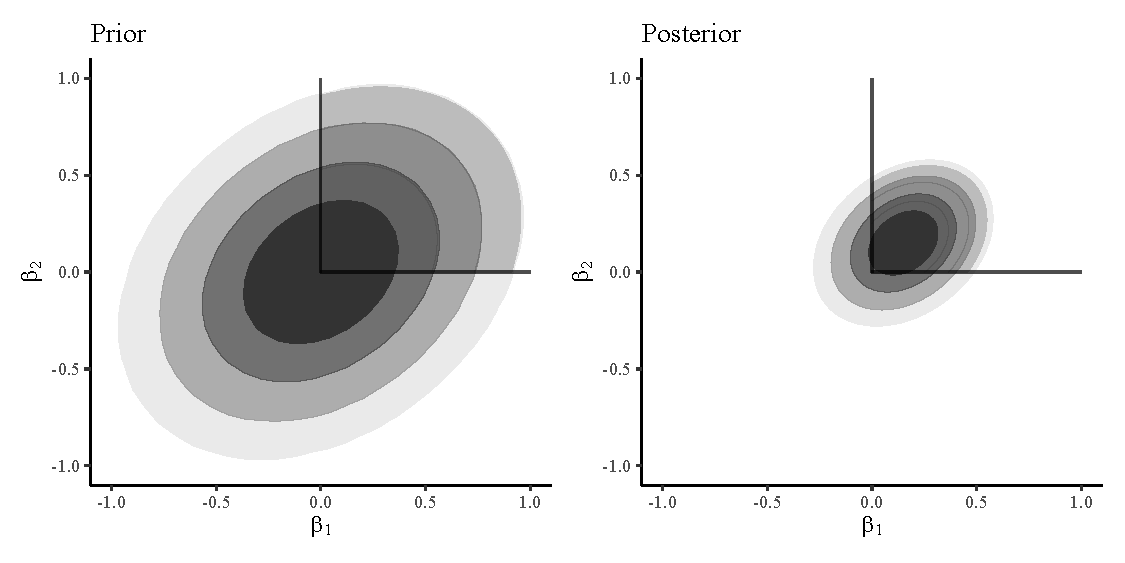
\includegraphics{thesis_volker_files/figure-latex/density-1.pdf}
\caption{\label{fig:density}Prior and posterior density for two regression parameters.}
\end{figure}

\setlength{\parindent}{0.2in}
\setlength{\leftskip}{0in}

\noindent

The conceptual idea of encompassing prior and posterior distributions is graphically depicted in Figure \ref{fig:density} (see, e.g., \protect\hyperlink{ref-volker_bes_2022}{Volker 2022} for a more technical exposition).
This figure shows the joint prior and posterior distribution for two regression coefficients, under an unconstrained hypothesis.
If, for the sake of exposition, we assume that we are interested in an informative hypothesis \(H_i: \{\beta_1, \beta_2\} > 0\) (stating that both regression coefficients are positive), the shaded areas in the upper right quadrants reflect the proportions of the prior and posterior in line with the hypothesis of interest.
The left-sided panel shows the prior distribution, centered at the constraints imposed by the hypothesis.
Given that the regression coefficients are slightly correlated, about \(30\%\) of the prior is in accordance with the hypothesis \(H_i\), indicating that this hypothesis has a complexity of about \(0.3\).
The right-hand figure shows the posterior distribution, centered at the posterior estimates of the regression coefficients.
It can be seen that the variance drastically decreased by combining the prior and the likelihood (e.g., the density is condensed), but that the shape remained the same.
Since the posterior estimates are quite in line with the hypothesis, the proportion of the posterior that is in line with the hypothesis is much larger as compared to the prior.
In fact, about \(75\%\) of the posterior distribution is in line with the specified hypothesis, resulting in a fit of \(0.75\).

Based on the notion of fit and complexity, the Bayes factor boils down to a relatively simple expression.
The Bayes factor of hypothesis \(H_i\) versus the unconstrained hypothesis is defined by
\[
BF_{i,u} = \frac{m(Y | X, H_{i})}{m(Y|X, H_{u})} = \frac{f_i}{c_i}.
\]
Returning to the aforementioned hypothetical example, comparing the hypothesis of interest with an unconstrained hypothesis yields a Bayes factor of \(BF_{i,u} = \frac{0.75}{0.3} = 2.5\).
Conventionally, rules of thumb for interpreting the size of the Bayes factor have been provided by \protect\hyperlink{ref-kass_raftery_bayes_factors_1995}{Kass and Raftery} (\protect\hyperlink{ref-kass_raftery_bayes_factors_1995}{1995}): \(1 < BF_{i,i'} < 3\) indicates unconvincing support for hypothesis \(H_i\) over \(H_{i'}\), \(BF_{i,i'}>3\) indicates substantial support, \(BF_{i,i'}>10\) yields strong support, and \(BF_{i,i'}>100\) indicates decisive support, although these rules are not strict and context dependent (\protect\hyperlink{ref-gu_approximated_2018}{Gu et al. 2018}).
Note, for example, that these benchmarks are generally inappropriate when evaluating an informative hypothesis against an unconstrained hypothesis, because the corresponding Bayes factor has an upper bound determined by the complexity.
Accordingly, when the informative hypothesis has a perfect fit, the maximum Bayes factor cannot exceed \(BF_{i,u} = \frac{1}{c_i}\).

The Bayes factor quantifies the fit of the data to the hypothesis, while accounting for how specific this hypothesis is.
When comparing two informative hypotheses \(H_i\) and \(H_{i'}\), the Bayes factor can be defined with reference to this relatively simple measure, such that
\[
BF_{i,i'} = \frac{BF_{i,u}}{BF_{i',u}} = \frac{f_i}{c_i} / \frac{f_{i'}}{c_{i'}}.
\]
The Bayes factor thus allows to evaluate multiple competing hypotheses and quantify the support for each hypothesis.
In the current study, the informative hypotheses of interest are evaluated against their corresponding complements.
The complement of an informative hypothesis is the parameter space that is \emph{not} in line with the hypothesis of interest.
The corresponding Bayes factor is then defined by
\[
BF_{i, ic} = \frac{BF_{i,u}}{BF_{ic,u}} = \frac{f_i}{c_i} / \frac{f_{ic}}{c_{ic}} = \frac{f_i}{c_i} / \frac{1 - f_{i}}{1 - c_{i}}.
\]
Given our current specification, it is easy to see that the complexity of the hypotheses under consideration equals the prior probability that \(\beta_j > 0\), which renders \(c_i = 0.5\), given that our prior distribution is symmetrically centered around 0.
Since we compare the hypotheses of interest versus their complements, the corresponding Bayes factors are given by
\[
BF_{i,ic} = \frac{f_i}{0.5} / \frac{f_{ic}}{0.5} = \frac{f_i}{f_{ic}} = \frac{f_i}{1-f_i}. 
\]
Additionally, we compare the hypotheses of interest with the unconstrained hypothesis, placing no constraints on the parameters, as this yields a more conservative evaluation of the hypothesis of interest over studies.
It is easy to see that testing against an unconstrained hypothesis is more conservative, as the Bayes factor when testing against an unconstrained hypothesis has an upper bound of \(\frac{1}{c_i}\), but a lower bound of \(0\), which indicates infinitely more support for the unconstrained hypothesis than for the hypothesis of interest.
Evidence against the hypothesis of interest thus weights heavier than evidence in favor of the hypothesis of interest.
When evaluating against the complement hypothesis, the Bayes factor has no upper bound.
With a perfectly fitting hypothesis, the fit of the complement tends to \(0\), and both positive and negative evidence is weighted equally.

It can be convenient to express the support for hypotheses not in terms of the Bayes factor itself, but in terms of posterior model probabilities.
Posterior model probabilities quantify the support for each of the hypotheses under consideration on a scale from \(0\) to \(1\), in such a way that the posterior model probabilities of all hypotheses combined sum to \(1\). To obtain posterior model probabilities, the Bayes factors are combined with prior model probabilities, reflecting the a priori plausibility of each hypothesis under consideration (i.e., before observing the data).
The posterior model probabilities for hypothesis \(H_i\) are given by
\[
PMP(H_{i}) = \frac{\pi_i BF_{i,u}}{\sum^m_{i'=1} \pi_{i'} BF_{i',u}},
\]
where \(m\) is the total number of hypotheses under consideration and \(\pi_i\) indicates the prior model probability of hypothesis \(H_i\).
The posterior model probabilities render the relative support for the hypotheses under consideration \emph{after} observing the data.

If there are multiple studies that assess a conceptually similar hypothesis, such as in our case, the support for this hypothesis can be aggregated over the separate studies using Bayesian Evidence Synthesis (\emph{BES}).
Namely, each of the studies provides some support for, or against, this overall hypothesis.
\emph{BES} statistically aggregates the support for the hypotheses under consideration by updating the prior model probabilities.
After analyzing the first study, the support for the hypothesis can be expressed in terms of posterior model probabilities.
These posterior model probabilities can be used as \emph{prior} model probabilities for the second study, resulting in the evidence for (or against) the hypothesis in the first two studies combined.
The resulting posterior model probabilities can again be used as prior model probabilities in the third study, and so on.

Hence, formally, the posterior model probabilities after study \(j\) are used as prior model probabilities in study \(j + 1\) (\protect\hyperlink{ref-kuiper_combining_2013}{Kuiper et al. 2013}).
Independent of the order of updating, repeating this process for \(J\) studies yields
\[
PMP(H_i)^J = \frac{\pi^0_{i} \prod^J_{j=1} BF^j_{i,u}}{\sum^m_{i'=1} \pi^0_{i'} \prod^J_{j=1} BF^j_{i',u}},
\]
where \(\pi^0_i\) indicates the prior model probabilities for hypothesis \(H_i\) before any study has been conducted.
To stay neutral with respect to the hypotheses of interest and their complements, a priori, we specify equal initial prior model probabilities for all hypotheses and their complements.
In our setup, we always compare the hypothesis of interest \(H_i: \beta_k > 0\) versus its complement \(H_{ic}: \beta_k \leq 0\) and the unconstrained hypothesis \(H_u: \beta_k\).
Accordingly, given equal initial prior model probabilities and only two hypotheses under comparison per evaluation, the posterior model probabilities after aggregating over all studies yield\footnote{
  The fit and the complexity of the unconstrained hypothesis are both equal to \(1\), such that the aggregated Bayes factor over multiple studies likewise equals \(1\). When evaluating against the complement, each \(BF^j_{i,u}\) can be divided by each \(BF^j_{c,u}\), which yields the Bayes factor against the complement hypothesis. Dividing \(BF^j_{c,u}\) in the denominator by itself renders the \(1\) in this equation as well.}
\[
PMP_{i,u}^J = \frac{\prod^J_{j=1}BF^j_{i,u}}{1 + \prod^J_{j=1} BF^j_{i,u}}, ~~~~~
PMP_{i,c}^J = \frac{\prod^J_{j=1}BF^j_{i,c}}{1 + \prod^J_{j=1} BF^j_{i,c}}.
\]
The posterior model probabilities after analyzing the data from all studies yield the relative plausibility that there indeed is a positive network control effect versus the unconstrained hypothesis, and versus no, or a negative, network control effect (i.e., the complement hypothesis).
With this procedure, we are able to quantify the evidence in favor of, or against, our hypothesis, in all studies combined, rather than in each of the studies individually.

\hypertarget{results}{%
\section{Results}\label{results}}

We first describe our results on first round behavior in the data from the individual studies.
Subsequently, we showcase how Bayesian Evidence Synthesis can be employed to aggregate the results over studies.
After the overall synthesis of results, we present separate results for trustfulness, trustworthiness and cooperation according to our hypotheses.
In addition, conform our distinction between two categories of studies, we consider studies with on the one hand random partner matching and on the other hand games played in triads.
We also aggregate the results of the studies within each subset.
We solely report Bayes factors and posterior model probabilities. The coefficients of the main analyses and of the robustness checks can be found in Table \ref{tab:ests-robust} in Appendix \ref{AppB}.

\hypertarget{results-in-individual-studies}{%
\subsection{Results in individual studies}\label{results-in-individual-studies}}

We describe the results for trustfulness (Hypothesis \(H_1\)) and trustworthiness (Hypothesis \(H_2\)) in the individual studies, and the difference in evidence between the two (Conjecture 1), followed by the results on cooperation (Hypothesis \(H_3\)).
We consistently start with the studies with random partner matching (set one), followed by the studies played in triads (set two).

\textbf{Trustfulness} \hspace{8pt} First round trustfulness rates are higher under network embeddedness than in the absence of network embeddedness in all three experiments in set one.
The corresponding evidence is therefore in favor of the network control hypothesis in all three studies, with Bayes factors that are all greater than \(1\).
For the data by \protect\hyperlink{ref-bolton_electronic_2004}{Bolton et al.} (\protect\hyperlink{ref-bolton_electronic_2004}{2004}), the network control hypothesis obtains \(BF_{i,u} = 1.47\) times more support than the unconstrained hypothesis, and \(BF_{i,c} = 2.80\) times more support than the complement hypothesis.
The experiments by \protect\hyperlink{ref-duffy2013social}{Duffy et al.} (\protect\hyperlink{ref-duffy2013social}{2013}) render Bayes factors of \(BF_{i,u} = 1.29\) and \(BF_{i,c} = 1.83\) in the minimum versus no network embeddedness sessions, and \(BF_{i,u} = 1.80\) and \(BF_{i,c} = 8.96\) in the full versus no network embeddedness sessions, and thus also support the network control hypothesis.

\renewcommand{\floatpagefraction}{.8}

\begin{table}

\caption{\label{tab:desc-table}Trustfulness and trustworthiness rates or cooperation rates for each of the studies considered, with corresponding Bayes factors against the respective unconstrained and complement alternative hypotheses.}
\centering
\begin{tabular}[t]{llrrrr}
\toprule
Study & Outcome & No Network & Network & $BF_{i,u}$ & $BF_{i,c}$\\
\midrule
\protect\hyperlink{ref-bolton_electronic_2004}{Bolton et al.} (\protect\hyperlink{ref-bolton_electronic_2004}{2004}) & Trustfulness & 0.67 & 0.75 & 1.47 & 2.80\\
\addlinespace
 & Trustworthiness & 0.69 & 0.61 & 0.64 & 0.47\\
\addlinespace
\protect\hyperlink{ref-duffy2013social}{Duffy et al.} (\protect\hyperlink{ref-duffy2013social}{2013}) & Trustfulness & 0.62 & 0.64 & 1.29 & 1.83\\
\addlinespace
No-NetMin & Trustworthiness & 0.68 & 0.77 & 1.82 & 10.32\\
\addlinespace
\protect\hyperlink{ref-duffy2013social}{Duffy et al.} (\protect\hyperlink{ref-duffy2013social}{2013}) & Trustfulness & 0.75 & 0.86 & 1.80 & 8.96\\
\addlinespace
No-NetFull & Trustworthiness & 0.62 & 0.94 & 2.00 & 2.60e+04\\
\addlinespace
\protect\hyperlink{ref-buskens_raub_veer_triads_2010}{Buskens et al.} (\protect\hyperlink{ref-buskens_raub_veer_triads_2010}{2010}) & Trustfulness & 0.83 & 0.94 & 1.85 & 12.17\\
\addlinespace
 & Trustworthiness & 0.87 & 0.94 & 1.68 & 5.25\\
\addlinespace
\protect\hyperlink{ref-miltenburg_buskens_triads_2012}{Van Miltenburg et al.} (\protect\hyperlink{ref-miltenburg_buskens_triads_2012}{2012}) & Trustfulness & 0.90 & 0.88 & 0.67 & 0.51\\
\addlinespace
 & Trustworthiness & 0.90 & 0.91 & 1.11 & 1.26\\
\addlinespace
\protect\hyperlink{ref-frey_buskens_investments_2019}{Frey et al.} (\protect\hyperlink{ref-frey_buskens_investments_2019}{2019}) & Trustfulness & 0.77 & 0.81 & 1.43 & 2.49\\
\addlinespace
 & Trustworthiness & 0.67 & 0.88 & 2.00 & 1.01e+03\\
\addlinespace
\protect\hyperlink{ref-barrera_buskens_third_2009}{Barrera and Buskens} (\protect\hyperlink{ref-barrera_buskens_third_2009}{2009}) & Trustfulness & 0.73 & 0.70 & 0.48 & 0.32\\
\addlinespace
 & Trustworthiness & 0.46 & 0.50 & 1.45 & 2.63\\
\addlinespace
\protect\hyperlink{ref-seinen_schram_social_2006}{Seinen and Schram} (\protect\hyperlink{ref-seinen_schram_social_2006}{2006}) & Cooperation (helping) & 0.38 & 0.61 & 1.90 & 19.35\\
\addlinespace
\protect\hyperlink{ref-corten_etal_reputation_2016}{Corten et al.} (\protect\hyperlink{ref-corten_etal_reputation_2016}{2016}) & Cooperation & 0.49 & 0.37 & 0.10 & 0.05\\
\bottomrule
\end{tabular}
\end{table}

In the second set of studies, \protect\hyperlink{ref-buskens_raub_veer_triads_2010}{Buskens et al.} (\protect\hyperlink{ref-buskens_raub_veer_triads_2010}{2010}) and \protect\hyperlink{ref-frey_buskens_investments_2019}{Frey et al.} (\protect\hyperlink{ref-frey_buskens_investments_2019}{2019}) find higher first-round trustfulness rates with network embeddedness than without, resulting in Bayes factors larger than one (\(BF_{i,u} = 1.85\) and \(BF_{i,c} = 12.17\), and \(BF_{i,u} = 1.43\) and \(BF_{i,c} = 2.49\), respectively).
In \protect\hyperlink{ref-miltenburg_buskens_triads_2012}{Van Miltenburg et al.} (\protect\hyperlink{ref-miltenburg_buskens_triads_2012}{2012}) and \protect\hyperlink{ref-barrera_buskens_third_2009}{Barrera and Buskens} (\protect\hyperlink{ref-barrera_buskens_third_2009}{2009}), on the contrary, trustfulness is higher in the absence of network embeddedness than under network embeddedness.
Hence, the Bayes factors for these experiments are smaller than one, rendering support against the network control hypothesis (\(BF_{i,u} = 0.67\) and \(BF_{i,c} = 0.51\) in \protect\hyperlink{ref-miltenburg_buskens_triads_2012}{Van Miltenburg et al. 2012}; \(BF_{i,u} = 0.48\) and \(BF_{i,c} = 0.32\) in \protect\hyperlink{ref-barrera_buskens_third_2009}{Barrera and Buskens 2009}).
Hence, we find consistent support for the network control hypothesis for trustfulness (\(H_1\)) in the first set of studies, while the second set yields inconsistent results.

\textbf{Trustworthiness} \hspace{8pt} The data by \protect\hyperlink{ref-bolton_electronic_2004}{Bolton et al.} (\protect\hyperlink{ref-bolton_electronic_2004}{2004}) provides support against the network control hypothesis for trustworthiness, in favor of the unconstrained (\(BF_{i,u} = 0.64\)) and complement (\(BF_{i,c} = 0.47\)) hypotheses.
Both experiments by \protect\hyperlink{ref-duffy2013social}{Duffy et al.} (\protect\hyperlink{ref-duffy2013social}{2013}) support the network control hypothesis, with more trustworthiness under network embeddedness than in the absence of network embeddedness.
The corresponding Bayes factors are \(BF_{i,u} = 1.82\) and \(BF_{i,c} = 10.32\) for the minimal versus no network embeddedness sessions, and \(BF_{i,u} = 2.00\) and \(BF_{i,c} = 2.60e+04\) for the full versus no network embeddedness sessions.
With \protect\hyperlink{ref-buskens_raub_veer_triads_2010}{Buskens et al.} (\protect\hyperlink{ref-buskens_raub_veer_triads_2010}{2010}), \protect\hyperlink{ref-miltenburg_buskens_triads_2012}{Van Miltenburg et al.} (\protect\hyperlink{ref-miltenburg_buskens_triads_2012}{2012}), \protect\hyperlink{ref-frey_buskens_investments_2019}{Frey et al.} (\protect\hyperlink{ref-frey_buskens_investments_2019}{2019}) and \protect\hyperlink{ref-barrera_buskens_third_2009}{Barrera and Buskens} (\protect\hyperlink{ref-barrera_buskens_third_2009}{2009}) finding more trustworthiness under network embeddedness than in the absence of network embeddedness, the network control hypothesis obtains between \(1.11\) and \(2.00\) times more support than the unconstrained hypothesis, and between \(1.26\) and \(1.01e+03\) times more support than the complement hypothesis.
Hence, the first set of studies yields inconsistent results, whereas the second set of studies consistently supports the network control hypothesis for trustworthiness (\(H_2\)).

\textbf{Trustfulness versus trustworthiness} \hspace{8pt} Comparing the evidence for trustfulness and trustworthiness reveals that in the first set of studies, only the data from \protect\hyperlink{ref-bolton_electronic_2004}{Bolton et al.} (\protect\hyperlink{ref-bolton_electronic_2004}{2004}) yields a larger Bayes factor for the network control hypothesis for trustfulness than for trustworthiness.
In the second set of studies, only the data from \protect\hyperlink{ref-buskens_raub_veer_triads_2010}{Buskens et al.} (\protect\hyperlink{ref-buskens_raub_veer_triads_2010}{2010}) yields more evidence for a network control effect on trustfulness than for a network control effect on trustworthiness.
The data from the six other experimental tests of a network control effect provide more evidence for a network control effect on trustworthiness than on trustfulness.
Hence, on the level of the individual studies, the amount of evidence for a network control effect on trustworthiness exceeds the evidence for trustfulness, in line with Conjecture 1.

\textbf{Cooperation} \hspace{8pt} \protect\hyperlink{ref-seinen_schram_social_2006}{Seinen and Schram} (\protect\hyperlink{ref-seinen_schram_social_2006}{2006}) and \protect\hyperlink{ref-corten_etal_reputation_2016}{Corten et al.} (\protect\hyperlink{ref-corten_etal_reputation_2016}{2016}) assessed cooperation in a Helping Game and Prisoner's Dilemma Game, respectively.
In \protect\hyperlink{ref-seinen_schram_social_2006}{Seinen and Schram} (\protect\hyperlink{ref-seinen_schram_social_2006}{2006}), there is substantially more cooperation with network embeddedness than without, reflected by relatively large Bayes factors (i.e., \(BF_{i,u} = 1.90\) and \(BF_{i,c} = 19.35\)).
\protect\hyperlink{ref-corten_etal_reputation_2016}{Corten et al.} (\protect\hyperlink{ref-corten_etal_reputation_2016}{2016}) find more cooperation in the absence of network embeddedness than under network embeddedness, resulting in Bayes factors that are substantially smaller than \(1\) (\(BF_{i,u} = 0.10\) and \(BF_{i,c} = 0.05\)).
Hence, individual studies provide inconsistent results for network control effects on cooperation (\(H_3\)).

\textbf{Robustness checks} \hspace{8pt} The above analyses were also performed with multilevel regression instead of one-level regression models with cluster-adjusted standard errors (see Appendix \ref{AppB}).
Substantively this yields the same results, although the evidence, for or against, the hypothesis tends to increase in size.
That is, evidence for the hypothesis of interest tends to become stronger (which happens in 6 out of 8 experiments that show a positive effect of network control opportunities for which a robustness check was done), while evidence against the hypothesis of interest tends to become more negative (which happens in 2 out of 3 experiments with a multilevel structure that show a negative effect of network control opportunities).
Hence, although some inconsistencies remain there is considerable support for our hypotheses and conjecture over the whole on the level of the individual studies, regardless of the statistical model used.

\hypertarget{aggregating-results-over-studies-using-bayesian-evidence-synthesis}{%
\subsection{Aggregating results over studies using Bayesian Evidence Synthesis}\label{aggregating-results-over-studies-using-bayesian-evidence-synthesis}}

After analyzing the individual studies, the results can be aggregated using Bayes Evidence Synthesis (Table \ref{tab:aggr-table}), as each of the studies under consideration provides some evidence for the network control hypothesis.
When aggregating over all individual tests, the network control hypothesis obtains \(7.27\) times more support than than the unconstrained hypothesis (Table \ref{tab:aggr-table}).
The resulting posterior model probability is equal to \(PMP_{i,u} = 0.88\) over all studies combined, rendering more support for the network control hypothesis than for the unconstrained hypothesis.
Moreover, the network control hypothesis obtains substantially more support than the complement alternative hypothesis.
That is, a positive network control effect is more than 500 billion times more likely than a negative network control effect, which renders a posterior model probability of about one.
Although the difference might seem remarkable, it should be noted that in every study, the Bayes factor versus the unconstrained hypothesis has an upper bound of \(1/c_i = 1/0.5 = 2\), but can approach \(0\) corresponding with infinite support for the unconstrained hypothesis.
When evaluating against the unconstrained hypothesis, evidence against a hypothesis weighs much heavier than evidence for this hypothesis, which may result in undesirable behavior when performing \emph{BES} (\protect\hyperlink{ref-volker_bes_2022}{Volker 2022}).
In fact, when evaluated against the unconstrained hypothesis, the study by \protect\hyperlink{ref-corten_etal_reputation_2016}{Corten et al.} (\protect\hyperlink{ref-corten_etal_reputation_2016}{2016}) provides such strong evidence against the hypothesis of interest that adding three experiments that fully support the hypothesis of interest (resulting in three Bayes factors of \(BF_{i,u} = 2\)) would still render more support for the unconstrained hypothesis.
Evaluating against the complement hypothesis weighs evidence for and against the network control hypothesis equally heavy, and provides tremendous support for the network control hypothesis.

\begin{table}

\caption{\label{tab:aggr-table}Aggregated Bayes factors and posterior model probabilities for the network control hypothesis for different outcomes and different (sub)sets of studies.}
\centering
\begin{tabu} to \linewidth {>{\raggedright\arraybackslash}p{15em}>{\raggedright\arraybackslash}p{3.25em}>{\raggedright\arraybackslash}p{3.25em}>{\raggedright\arraybackslash}p{4.25em}>{\raggedright\arraybackslash}p{4.25em}>{\raggedright\arraybackslash}p{7em}}
\toprule
  & $BF_{i,u}$ & $PMP_{i,u}$ & $BF_{i,c}$ & $PMP_{i,c}$ & Amount of support\\
\midrule
All studies and outcomes combined & 7.27 & 0.88 & 5.23e+11 & 1.00 & Very strong\\
\addlinespace
 &  &  &  &  \vphantom{2} & \\
\addlinespace
Trustfulness ($H_1$) & 2.94 & 0.75 & 224.06 & 1.00 & Strong\\
\addlinespace
\hspace{8pt}Random partner matching & 3.43 & 0.77 & 45.77 & 0.98 & Substantial\\
\addlinespace
\hspace{8pt}Triads & 0.86 & 0.46 & 4.90 & 0.83 & Positive\\
\addlinespace
 &  &  &  &  \vphantom{1} & \\
\addlinespace
Trustworthiness ($H_2$) & 12.71 & 0.93 & 2.24e+09 & 1.00 & Very strong\\
\addlinespace
\hspace{8pt}Random partner matching & 2.34 & 0.70 & 1.27e+05 & 1.00 & Very strong\\
\addlinespace
\hspace{8pt}Triads & 5.43 & 0.84 & 1.76e+04 & 1.00 & Very strong\\
\addlinespace
 &  &  &  &  & \\
\addlinespace
Cooperation ($H_3$) & 0.19 & 0.16 & 1.04 & 0.51 & Undecisive\\
\bottomrule
\end{tabu}
\end{table}

We now assess the support for the network control hypothesis separately for trustfulness, trustworthiness and cooperation, and additionally distinguish between experiments with random partner matching and with triads.

\textbf{Trustfulness} \hspace{8pt} When considering the evidence for the network control hypothesis for trustfulness over all studies, we find that the network control hypothesis provides a better fit to the data than the unconstrained hypothesis, although the amount of evidence is not overwhelming.
The network control hypothesis obtains \(BF_{i,u} = 2.94\) times more support than the unconstrained hypothesis, which renders a posterior probability of \(PMP_{i,u} = 0.75\) that the network control hypothesis is a more accurate hypothesis than the unconstrained hypothesis (Table \ref{tab:aggr-table}).
Note, however, that evidence against the network control hypothesis again weighs heavier than evidence for this hypothesis when comparing against the unconstrained hypothesis.
Comparing against the complement hypothesis renders strong support for the network control hypothesis for trustfulness (\(BF_{i,c} = 224.06\); \(PMP_{i,c} = 1.00\)).

We further assess the evidence for the network control hypothesis for trustfulness distinctly for experiments with random partner matching and experiments with triads.
Under random partner matching, the aggregated evidence shows that the network control hypothesis obtains \(BF_{i,u} = 3.43\) times more support than the unconstrained hypothesis, and \(BF_{i,c} = 45.77\) times more support than the complement hypothesis.
In terms of posterior model probabilities, this yields \(PMP_{i,u} = 0.77\) and \(PMP_{i,c} = 0.98\).
In the studies in triads, the unconstrained hypothesis obtains more support than the network control hypothesis (\(BF_{i,u} = 0.86\); \(PMP_{i,u} = 0.46\)), which is not extremely surprising as two of the studies in this set find evidence against the network control hypothesis for trustfulness.
However, the network control hypothesis obtains more support than its complement (\(BF_{i,c} = 4.90\); \(PMP_{i,c} = 0.83\)), although the aggregated support is not too convincing in this set.
Hence, although there is strong support for the network control hypothesis for trustfulness (\(H_1\)) in both sets of studies combined, this result stems predominantly from the consistent results in the first set.
In the studies in triads, there is no consistent support for this hypothesis.

\textbf{Trustworthiness} \hspace{8pt}The results for the network control effect on trustworthiness are more consistent, and therefore the aggregation procedure renders very strong evidence for Hypothesis \(H_2\).
Aggregated over all studies combined, the network control hypothesis obtains \(BF_{i,u} = 12.71\) times more support than the unconstrained hypothesis (\(PMP_{i,u} = 0.93\)), and \(BF_{i,c} = 2.24e+09\) times more than the complement (\(PMP_{i,c} = 1.00\)).
Also in both distinct sets of studies, there is considerable support for the network control hypothesis.
In the first set, the support in \protect\hyperlink{ref-duffy2013social}{Duffy et al.} (\protect\hyperlink{ref-duffy2013social}{2013}) outweighs the lack of support for the network control hypothesis in \protect\hyperlink{ref-bolton_electronic_2004}{Bolton et al.} (\protect\hyperlink{ref-bolton_electronic_2004}{2004}).
This renders the network control hypothesis \(BF_{i,u} = 2.34\) times more plausible than the unconstrained hypothesis (\(PMP_{i,u} = 0.70\)) and \(BF_{i,c} = 1.27e+05\) times more plausible the complement (\(PMP_{i,c} = 1.00\)) in this first set.
As the results were consistent in the experiments with triads, the network control hypothesis is strongly supported, regardless of whether we compare against the unconstrained (\(BF_{i,u} = 5.43\); \(PMP_{i,u} = 0.84\)) or the complement hypothesis (\(BF_{i,c} = 1.76e+04\); \(PMP_{i,c} = 1.00\)).

\textbf{Trustfulness versus trustworthiness} \hspace{8pt} With respect to Conjecture 1, we find that there is indeed more evidence over all studies for a network control effect on trustworthiness than for this effect on trustfulness, as shown by the large difference between the aggregated Bayes factors for trustfulness and trustworthiness.
The same pattern appears within the two subsets.
Although in studies with random partner matching, there is slightly more evidence for the network control hypothesis for trustfulness than for trustworthiness when evaluated against the unconstrained (\(BF_{i,u} = 3.43\) versus \(BF_{i,u} = 2.34\), respectively), comparing against the complement (\(BF_{i,c} = 45.77\) versus \(BF_{i,c} = 1.27e+05\)) yields more support for the network control hypothesis for trustworthiness.
Hence, on the level of the individual studies and on the aggregate level, there is more evidence for a network control effect on trustworthiness than on trustfulness, in line with Conjecture 1.

\textbf{Cooperation} \hspace{8pt}When aggregating over the studies on cooperation, we find little support for a network control effect.
Whereas the data from \protect\hyperlink{ref-seinen_schram_social_2006}{Seinen and Schram} (\protect\hyperlink{ref-seinen_schram_social_2006}{2006}) provides substantial support for a network control effect, data from \protect\hyperlink{ref-corten_etal_reputation_2016}{Corten et al.} (\protect\hyperlink{ref-corten_etal_reputation_2016}{2016}) yields the opposite.
Accordingly, there is more support for the unconstrained hypothesis than for the network control hypothesis (\(BF_{i,u} = 0.19\); \(PMP_{i,u} = 0.16\)), while the evidence for the network control hypothesis and its complement are rather balanced (\(BF_{i,c} = 1.04\); \(PMP_{i,c} = 0.51\)).
Note, however, that in the study by \protect\hyperlink{ref-corten_etal_reputation_2016}{Corten et al.} (\protect\hyperlink{ref-corten_etal_reputation_2016}{2016}), the participants played, on average, 16 iterations of a Prisoner's Dilemma game with each other participant in their network, and obtained information on all interactions they engaged in themselves, resulting in substantial dyadic embeddedness.
In \protect\hyperlink{ref-seinen_schram_social_2006}{Seinen and Schram} (\protect\hyperlink{ref-seinen_schram_social_2006}{2006}), the amount of dyadic embeddedness in the condition without network embeddedness was much lower, as the participants played about 100 rounds of the Helping Game in a network of size \(16\), without being informed at all about past choices of a current partner, which impedes conditioning on a partner's past behavior.

\textbf{Robustness checks} \hspace{8pt} Analyses on the robustness of the results by modelling the data with multilevel regression models instead of using cluster-adjusted standard errors have important implications.
Because the evidence tends to become more extreme when fitting multilevel models, regardless of whether the evidence supports or contradict the network control hypothesis, the aggregated support against the unconstrained hypothesis decreases substantially (Appendix \ref{AppB}).
When comparing against the unconstrained hypothesis, the experiment by \protect\hyperlink{ref-barrera_buskens_third_2009}{Barrera and Buskens} (\protect\hyperlink{ref-barrera_buskens_third_2009}{2009}) provides so much evidence against the network control hypothesis for trustfulness that all other studies combined can hardly compensate, resulting in little support on the aggregate level (\(BF_{i,u} = 2.66\); \(PMP_{i,u} = 0.73\)).
When comparing against the complement, the evidence for and against the hypothesis of interest are weighted equally such that the issue dissolves, and the support for the network control hypothesis by far outweighs support for the complement alternative (\(BF_{i,c} = 9.90e+17\); \(PMP_{i,u} = 1.00\)).
This issue also occurs when solely aggregating the support for trustfulness.
Evaluating against the unconstrained hypothesis renders most support for the unconstrained hypothesis (\(BF_{i,u} = 0.61\); \(PMP_{i,u} = 0.38\)), whereas evaluating against the complement hypothesis renders substantial support for the network control hypothesis (\(BF_{i,c} = 3.74e+03\); \(PMP_{i,c} = 1.00\)).
When zooming in on trustfulness in the studies with participants interacting in triads, the evidence for the network control effect substantially decreases, also when comparing against the complement hypothesis.
Within this subset the unconstrained hypothesis obtains more support than the network control hypothesis (\(BF_{i,u} = 0.12\); \(PMP_{i,u} = 0.11\)), while there is hardly evidence for the network control hypothesis over its complement (\(BF_{i,c} = 1.63\); \(PMP_{i,c} = 0.62\)).
Applying this robustness check for trustworthiness and cooperation has a negligible effect.

Apart from having a rather dramatic effect on the evidence for a network control effect on trustfulness in the studies in triads, the substantive conclusions remain the same throughout the robustness analysis.
In fact, except for trustfulness in the studies in triads, the evidence for the network control hypothesis evaluated against the complement becomes stronger in all subgroups considered.
Hence, our results provide substantial support for the network control hypothesis for trustfulness, and even more for trustworthiness.
When participants interacted in triads, the results for trustfulness are somewhat more ambiguous, just as the results for cooperation.

\hypertarget{discussion}{%
\section{Discussion}\label{discussion}}

Theoretically, network control opportunities provide ways to promote trust and cooperation in social and economic interactions.
Earlier research yielded inconsistent empirical findings on network control effects.
Using \emph{BES} to aggregate over available studies, we show that the network control hypotheses are overall substantially more likely than the unconstrained hypotheses, while there is no support whatsoever for the complement hypotheses.
When considering the specific hypotheses, we find strong support for the network control hypothesis on trustfulness.
Especially in the studies where network embeddedness was implemented without dyadic embeddedness, all evidence supports this hypothesis.
In the studies with network embeddedness implemented in the presence of dyadic embeddedness, the support was weaker and less consistent, but still positive when comparing with the complement hypothesis.
The results provide even more evidence for the network control hypothesis for trustworthiness, regardless of the set of studies.
Lastly, the results are doubtful for cooperation specifically.
As the two studies that assess cooperation show contradictory results, more data would be useful to assess this effect.
Yet, as there is substantial evidence for both trustfulness and trustworthiness, which are in essence the components that make up cooperation, it is plausible that network control holds for cooperation as well.

Considering the inconsistent results for trustfulness, one could argue that dyadic embeddedness already fosters trustfulness to a large extent (as shown by, e.g., \protect\hyperlink{ref-dal_buxf3_cooperation_2005}{Dal Bó 2005}; \protect\hyperlink{ref-dal_buxf3_fruxe9chette_determinants_2018}{Dal Bó and Fréchette 2018}), which is also reflected by trustfulness rates that are overall higher when network embeddedness is implemented with dyadic embeddedness.
Accordingly, there is simply less improvement possible when network control is `added' to dyadic control.
In most studies with network and dyadic embeddedness, the sanction opportunities provided by dyadic embeddedness may already provide sufficient incentives to place trust.
Moreover, if trustors do not take into account the benefits of dyadic sanctions, it may be doubtful whether they account for the benefit of sanctions placed by a third party.
Additionally, in the study by \protect\hyperlink{ref-barrera_buskens_third_2009}{Barrera and Buskens} (\protect\hyperlink{ref-barrera_buskens_third_2009}{2009}), trust may be lower because the condition with network and dyadic embeddedness was implemented \emph{before} the condition with solely dyadic embeddedness.
As a consequence, trustors may learn in the first condition that trust is seldom abused, allowing to be more trustful in the second condition.
Yet, the fact that trustworthiness is higher under network embeddedness may cast doubt about the plausibility of this explanation.

As we conjectured, there was more support for a network control effect for trustworthiness than for trustfulness.
This was the case for the aggregated results over all studies, and for the aggregated results in the two sets considered.
In both sets, the Bayes factor for the network control hypothesis versus its complement was larger for trustworthiness than for trustfulness.
Accordingly, it might indeed be more difficult for trustors than for trustees to anticipate on network control effects.
Trustees have to anticipate exclusively on potential future sanctions by third parties, while trustors have to anticipate also on how the trustee anticipates on those sanctions by third parties (\protect\hyperlink{ref-buskens_raub_veer_triads_2010}{Buskens et al. 2010}).
Especially if a trustor can personally retaliate an abuse of trust in future interactions, as under dyadic embeddedness, trustors may not reason an additional step ahead.

From a methodological viewpoint, we showed how \emph{BES} can be applied to aggregate the results from a heterogeneous set of studies on the same phenomenon, and how the results of \emph{BES} should be interpreted.
Additionally, we showed the difference between evaluating against an unconstrained hypothesis and the complement hypothesis, with the former being far more conservative.
Comparing against the unconstrained hypothesis when aggregating over studies yields that a single study with moderate support against a hypothesis can substantially reduce the aggregated support for that hypothesis, even if there are multiple studies supporting the hypothesized effect (see \protect\hyperlink{ref-volker_bes_2022}{Volker 2022} for a similar argument based on statistical simulations).
Evaluating against the complement hypothesis does not only provide a meaningful alternative, it also weighs evidence for and against the hypothesis of interest equally heavy, at least if the complexities of both hypotheses are equal.
Hence, in line with recommendations by \protect\hyperlink{ref-volker_bes_2022}{Volker} (\protect\hyperlink{ref-volker_bes_2022}{2022}), we suggest to evaluate informative hypotheses against their complements, rather than against unconstrained alternatives.

We only evaluated informative, inequality-constrained hypotheses, while evaluating equality-constrained hypotheses (as the classical null hypothesis) is still the standard in many areas of research.
When evaluating equality-constrained hypotheses, one should note that the Bayes factor, which depends on both the prior and the posterior distribution of the parameters, is much more sensitive to the specification of the prior distribution than when evaluating inequality-constrained hypotheses (\protect\hyperlink{ref-klugkist_bf_2007}{Klugkist and Hoijtink 2007}).
Additionally, under insufficient statistical power, the Bayes factor within individual studies tends to provide relatively large support for a null hypothesis (\protect\hyperlink{ref-tendeiro_kiers_2019}{Tendeiro and Kiers 2019}).
Future methodological research should extent the work by \protect\hyperlink{ref-hoijtink_prior_2021}{Hoijtink} (\protect\hyperlink{ref-hoijtink_prior_2021}{2021}), who assessed the sensitivity of the Bayes factor to the specification of the prior within a study, to the situation where researchers aggregate over multiple studies.
Lastly, whereas we had to reanalyze the data, this is no requirement for \emph{BES}, as it can evaluate a hypothesis on the basis of a parameter estimate and its accompanying standard error (\protect\hyperlink{ref-kuiper_combining_2013}{Kuiper et al. 2013}).
This does, however, require that the hypothesis of interest is evaluated and reported in the original study.

We solely relied on experimental studies that allowed to distinguish between network control and network learning effects, while these effects are often intertwined in observational studies.
That is, those who expect to interact in the future, may also be more likely to have a shared history, or at least have common acquaintances that can inform both parties on past behavior of the other.
Moreover, existing observational research on embeddedness effects generally used indicators for these effects that are unable to discriminate between learning and control effects (see, e.g., \protect\hyperlink{ref-buskens_raub_handbook_2013}{Buskens and Raub 2013} for an extensive overview).
To evaluate network control effects experimentally, we explicitly focused on first round behavior.
Yet, one could consider other ways of evaluating network control effects, for example by focusing on end-game effects (i.e., the behavior when sanction opportunities decrease, because the end of the interaction is near, while statistically controlling for learning effects, as in \protect\hyperlink{ref-bolton_electronic_2004}{Bolton et al. 2004}; \protect\hyperlink{ref-buskens_raub_veer_triads_2010}{Buskens et al. 2010}).
Evaluating such additional operationalizations of network control effects could add to the robustness of our findings.

An additional advantage of the experimental design is that it ensures that the choices participants make are related to material incentives, rather than hypothetical scenarios as in vignette or survey research.
Moreover, experimental designs facilitate to investigate the causal effect of network control opportunities.
Yet, the downsides of experimental studies have also been well documented (e.g., \protect\hyperlink{ref-falk_heckman_experiments_2009}{Falk and Heckman 2009}; \protect\hyperlink{ref-jackson_cox_experimental_2013}{Jackson and Cox 2013}).
Experimental studies often rely on an artificial and unrealistic setting, potentially posing problems to the generalizability of the results to real-world settings, while the participants are often undergraduate students.
However, the availability of experimental designs is no requirement when applying \emph{BES}.
As long as the studies under consideration assess a conceptually similar hypothesis, \emph{BES} is applicable, regardless of the study design, such that it can also be applied if one aims at a synthesis over studies with longitudinal, cross-sectional and experimental designs.
In fact, such variation is encouraged, because complementary tests allow to build a more robust body of evidence by aggregating evidence for, or against, hypotheses over different contexts (\protect\hyperlink{ref-jackson_cox_experimental_2013}{Jackson and Cox 2013}; \protect\hyperlink{ref-lawlor_triangulation_2017}{Lawlor et al. 2017}).

To summarize, we provided substantial evidence for a network control effect on trustfulness and trustworthiness, while there was more evidence for the latter compared to the former.
We thus established that sanction opportunities through third parties positively influence trust.
Our synthesis was only possible by employing \emph{BES}, which allows for a synthesis over heterogeneous studies.
As such, \emph{BES} enables researchers to aggregate the evidence for phenomena of interest over replications, which gives insight in the robustness of research findings.

\hypertarget{literature}{%
\section{Literature}\label{literature}}

\setlength{\parindent}{-0.2in}
\setlength{\leftskip}{0.2in}

\noindent

\hypertarget{refs}{}
\begin{CSLReferences}{1}{0}
\leavevmode\vadjust pre{\hypertarget{ref-anderhub_repeated_trust_2002}{}}%
Anderhub, Vital, Dirk Engelmann, and Werner Güth. 2002. {``An Experimental Study of the Repeated Trust Game with Incomplete Information.''} \emph{Journal of Economic Behavior \& Organization} 48(2):197--216. doi: \href{https://doi.org/10.1016/S0167-2681(01)00216-5}{10.1016/S0167-2681(01)00216-5}.

\leavevmode\vadjust pre{\hypertarget{ref-barrera_buskens_third_2009}{}}%
Barrera, Davide, and Vincent Buskens. 2009. {``Third-Party Effects.''} Pp. 37--72 in \emph{eTrust: {F}orming {R}elationships in the {O}nline {W}orld}. New York, NY: Russell Sage Foundation.

\leavevmode\vadjust pre{\hypertarget{ref-lme4}{}}%
Bates, Douglas, Martin Mächler, Ben Bolker, and Steve Walker. 2015. {``Fitting Linear Mixed-Effects Models Using {lme4}.''} \emph{Journal of Statistical Software} 67(1):1--48. doi: \href{https://doi.org/10.18637/jss.v067.i01}{10.18637/jss.v067.i01}.

\leavevmode\vadjust pre{\hypertarget{ref-berg_etal_trust_1995}{}}%
Berg, Joyce, John Dickhaut, and Kevin McCabe. 1995. {``Trust, Reciprocity, and Social History.''} \emph{Games and Economic Behavior} 10(1):122--42. doi: \href{https://doi.org/10.1006/game.1995.1027}{10.1006/game.1995.1027}.

\leavevmode\vadjust pre{\hypertarget{ref-binmore_playing_2007}{}}%
Binmore, Ken. 2007. \emph{Playing for Real: A Text on Game Theory}. New York, NY: Oxford {U}niversity {P}ress.

\leavevmode\vadjust pre{\hypertarget{ref-blau1964exchange}{}}%
Blau, Peter M. 1986. \emph{Exchange and Power in Social Life}. New York, NY: Routledge.

\leavevmode\vadjust pre{\hypertarget{ref-bohnet_learning_2005}{}}%
Bohnet, Iris, Heike Harmgart, Steffen Huck, and Jean-Robert Tyran. 2005. {``{Learning Trust}.''} \emph{Journal of the European Economic Association} 3(2-3):322--29. doi: \href{https://doi.org/10.1162/jeea.2005.3.2-3.322}{10.1162/jeea.2005.3.2-3.322}.

\leavevmode\vadjust pre{\hypertarget{ref-bohnet_huck_2004}{}}%
Bohnet, Iris, and Steffen Huck. 2004. {``Repetition and Reputation: Implications for Trust and Trustworthiness When Institutions Change.''} \emph{American Economic Review} 94(2):362--66. doi: \href{https://doi.org/10.1257/0002828041301506}{10.1257/0002828041301506}.

\leavevmode\vadjust pre{\hypertarget{ref-bolton_electronic_2004}{}}%
Bolton, Gary E., Elena Katok, and Axel Ockenfels. 2004. {``How Effective Are Electronic Reputation Mechanisms? An Experimental Investigation.''} \emph{Management Science} 50(11):1587--1602. doi: \href{https://doi.org/10.1287/mnsc.1030.0199}{10.1287/mnsc.1030.0199}.

\leavevmode\vadjust pre{\hypertarget{ref-buskens_trust_2003}{}}%
Buskens, Vincent. 2003. {``Trust in Triads: Effects of Exit, Control, and Learning.''} \emph{Games and Economic Behavior} 42(2):235--52. doi: \href{https://doi.org/10.1016/S0899-8256(02)00563-8}{10.1016/S0899-8256(02)00563-8}.

\leavevmode\vadjust pre{\hypertarget{ref-buskens2018trust}{}}%
Buskens, Vincent, Vincenz Frey, and Werner Raub. 2018. {``Trust Games: Game-Theoretic Approaches to Embedded Trust.''} Pp. 305--36 in \emph{The {O}xford {H}andbook of {S}ocial and {P}olitical {T}rust}. New York, NY: Oxford University Press.

\leavevmode\vadjust pre{\hypertarget{ref-buskens_raub_embedded_2002}{}}%
Buskens, Vincent, and Werner Raub. 2002. {``Embedded Trust: {Control} and Learning.''} Pp. 167--202 in \emph{Advances in {Group} {Processes}}. Vol. 19, \emph{Advances in {Group} {Processes}}. Emerald Group Publishing Limited.

\leavevmode\vadjust pre{\hypertarget{ref-buskens_raub_handbook_2013}{}}%
Buskens, Vincent, and Werner Raub. 2013. {``Rational Choice Research on Social Dilemmas: Embeddedness Effects on Trust.''} Pp. 113--50 in \emph{The {H}andbook of {R}ational {C}hoice {S}ocial {R}esearch}, edited by R. Wittek, T. A. B. Snijders, and V. Nee. Stanford, CA: Stanford University Press.

\leavevmode\vadjust pre{\hypertarget{ref-buskens_raub_veer_triads_2010}{}}%
Buskens, Vincent, Werner Raub, and Joris Van der Veer. 2010. {``Trust in Triads: An Experimental Study.''} \emph{Social Networks} 32(4):301--12. doi: \href{https://doi.org/10.1016/j.socnet.2010.05.001}{10.1016/j.socnet.2010.05.001}.

\leavevmode\vadjust pre{\hypertarget{ref-camerer2016evaluating}{}}%
Camerer, Colin F., Anna Dreber, Eskil Forsell, Teck-Hua Ho, Jürgen Huber, Magnus Johannesson, Michael Kirchler, Johan Almenberg, Adam Altmejd, Taizan Chan, Emma Heikensten, Felix Holzmeister, Taisuke Imai, Siri Isaksson, Gideon Nave, Thomas Pfeiffer, Michael Razen, and Hang Wu. 2016. {``Evaluating Replicability of Laboratory Experiments in Economics.''} \emph{Science} 351(6280):1433--36. doi: \href{https://doi.org/10.1126/science.aaf0918}{10.1126/science.aaf0918}.

\leavevmode\vadjust pre{\hypertarget{ref-camerer2018evaluating}{}}%
Camerer, Colin F., Anna Dreber, Felix Holzmeister, Teck-Hua Ho, Jürgen Huber, Magnus Johannesson, Michael Kirchler, Gideon Nave, Brian A. Nosek, Thomas Pfeiffer, Adam Altmejd, Nick Buttrick, Taizan Chan, Yiling Chen, Eskil Forsell, Anup Gampa, Emma Heikensten, Lily Hummer, Taisuke Imai, Siri Isaksson, Dylan Manfredi, Julia Rose, Eric-Jan Wagenmakers, and Hang Wu. 2018. {``Evaluating the Replicability of Social Science Experiments in Nature and Science Between 2010 and 2015.''} \emph{Nature Human Behaviour} 2(9):637--44. doi: \href{https://doi.org/10.1038/s41562-018-0399-z}{10.1038/s41562-018-0399-z}.

\leavevmode\vadjust pre{\hypertarget{ref-camerer_weigelt_sequential_1988}{}}%
Camerer, Colin F., and Keith Weigelt. 1988. {``Experimental Tests of a Sequential Equilibrium Reputation Model.''} \emph{Econometrica} 56(1):1--36. doi: \href{https://doi.org/10.2307/1911840}{10.2307/1911840}.

\leavevmode\vadjust pre{\hypertarget{ref-cohen_earth_1994}{}}%
Cohen, Jacob. 1994. {``The Earth Is Round (p{\enspace}\textless{}{\enspace}.05).''} \emph{American Psychologist} 49(12):997--1003. doi: \href{https://doi.org/10.1037/0003-066X.49.12.997}{10.1037/0003-066X.49.12.997}.

\leavevmode\vadjust pre{\hypertarget{ref-coleman_structure_1986}{}}%
Coleman, James S. 1986. {``Psychological Structure and Social Structure in Economic Models.''} \emph{The Journal of Business} 59(4):S365--69.

\leavevmode\vadjust pre{\hypertarget{ref-Cook2013}{}}%
Cook, Karen S., Coye Cheshire, Eric R. W. Rice, and Sandra" Nakagawa. 2013. {``Social Exchange Theory.''} Pp. 61--88 in \emph{Handbook of {S}ocial {P}sychology}, edited by J. DeLamater and A. Ward. Dordrecht: Springer Netherlands.

\leavevmode\vadjust pre{\hypertarget{ref-cooper_handbook_2009}{}}%
Cooper, Harris, Larry Vernon Hedges, and Jeffrey C. Valentine. 2009. \emph{The Handbook of Research Synthesis and Meta-Analysis}. 2nd ed. New York, NY: Russell Sage Foundation.

\leavevmode\vadjust pre{\hypertarget{ref-corten_etal_reputation_2016}{}}%
Corten, Rense, Stephanie Rosenkranz, Vincent Buskens, and Karen S. Cook. 2016. {``Reputation Effects in Social Networks Do Not Promote Cooperation: An Experimental Test of the Raub \& Weesie Model.''} \emph{PLOS ONE} 11(7):1--17. doi: \href{https://doi.org/10.1371/journal.pone.0155703}{10.1371/journal.pone.0155703}.

\leavevmode\vadjust pre{\hypertarget{ref-dal_buxf3_cooperation_2005}{}}%
Dal Bó, Pedro. 2005. {``Cooperation Under the Shadow of the Future: Experimental Evidence from Infinitely Repeated Games.''} \emph{The American Economic Review} 95(5):1591--1604. doi: \href{https://doi.org/10.1257/000282805775014434}{10.1257/000282805775014434}.

\leavevmode\vadjust pre{\hypertarget{ref-dal_buxf3_fruxe9chette_evolution_2011}{}}%
Dal Bó, Pedro, and Guillaume R. Fréchette. 2011. {``The Evolution of Cooperation in Infinitely Repeated Games: Experimental Evidence.''} \emph{American Economic Review} 101(1):411--29. doi: \href{https://doi.org/10.1257/aer.101.1.411}{10.1257/aer.101.1.411}.

\leavevmode\vadjust pre{\hypertarget{ref-dal_buxf3_fruxe9chette_determinants_2018}{}}%
Dal Bó, Pedro, and Guillaume R. Fréchette. 2018. {``On the Determinants of Cooperation in Infinitely Repeated Games: A Survey.''} \emph{Journal of Economic Literature} 56(1):60--114. doi: \href{https://doi.org/10.1257/jel.20160980}{10.1257/jel.20160980}.

\leavevmode\vadjust pre{\hypertarget{ref-dasgupta_1988}{}}%
Dasgupta, Partha. 1988. {``Trust as a Commodity.''} Pp. 49--72 in \emph{Trust: {M}aking and {B}reaking {C}ooperative {R}elations}, edited by D. Gambetta. Department of Sociology, University of Oxford.

\leavevmode\vadjust pre{\hypertarget{ref-duffy_cooperative_2009}{}}%
Duffy, John, and Jack Ochs. 2009. {``Cooperative Behavior and the Frequency of Social Interaction.''} \emph{Games and Economic Behavior} 66(2):785--812. doi: \href{https://doi.org/10.1016/j.geb.2008.07.003}{10.1016/j.geb.2008.07.003}.

\leavevmode\vadjust pre{\hypertarget{ref-duffy2013social}{}}%
Duffy, John, Huan Xie, and Yong-Ju Lee. 2013. {``Social Norms, Information, and Trust Among Strangers: Theory and Evidence.''} \emph{Economic Theory} 52(2):669--708. doi: \href{https://doi.org/10.1007/s00199-011-0659-x}{10.1007/s00199-011-0659-x}.

\leavevmode\vadjust pre{\hypertarget{ref-embrey_etal_cooperation_2018}{}}%
Embrey, Matthew, Guillaume R. Fréchette, and Sevgi Yuksel. 2018. {``{Cooperation in the Finitely Repeated Prisoner's Dilemma}.''} \emph{The Quarterly Journal of Economics} 133(1):509--51. doi: \href{https://doi.org/10.1093/qje/qjx033}{10.1093/qje/qjx033}.

\leavevmode\vadjust pre{\hypertarget{ref-engelmann_firschbacher_2009}{}}%
Engelmann, Dirk, and Urs Fischbacher. 2009. {``Indirect Reciprocity and Strategic Reputation Building in an Experimental Helping Game.''} \emph{Games and Economic Behavior} 67(2):399--407. doi: \url{https://doi.org/10.1016/j.geb.2008.12.006}.

\leavevmode\vadjust pre{\hypertarget{ref-falk_heckman_experiments_2009}{}}%
Falk, Armin, and James J. Heckman. 2009. {``Lab Experiments Are a Major Source of Knowledge in the Social Sciences.''} \emph{Science} 326(5952):535--38. doi: \href{https://doi.org/10.1126/science.1168244}{10.1126/science.1168244}.

\leavevmode\vadjust pre{\hypertarget{ref-frey_buskens_investments_2019}{}}%
Frey, Vincenz, Vincent Buskens, and Rense Corten. 2019. {``Investments in and Returns on Network Embeddedness: An Experiment with Trust Games.''} \emph{Social Networks} 56:81--92. doi: \href{https://doi.org/10.1016/j.socnet.2018.07.006}{10.1016/j.socnet.2018.07.006}.

\leavevmode\vadjust pre{\hypertarget{ref-bda2013}{}}%
Gelman, Andrew, John B. Carlin, Hal S. Stern, Aki Vehtari, and Donald B. Rubin. 2004. \emph{Bayesian Data Analysis}. 3rd ed. New York, NY: {Chapman and Hall/CRC}.

\leavevmode\vadjust pre{\hypertarget{ref-granovetter_economic_1985}{}}%
Granovetter, Mark. 1985. {``Economic Action and Social Structure: The Problem of Embeddedness.''} \emph{American Journal of Sociology} 91(3):481--510. doi: \href{https://doi.org/10.1086/228311}{10.1086/228311}.

\leavevmode\vadjust pre{\hypertarget{ref-bain}{}}%
Gu, Xin, Herbert Hoijtink, Joris Mulder, and Caspar J. van Lissa. 2020. \emph{Bain: Bayes Factors for Informative Hypotheses}.

\leavevmode\vadjust pre{\hypertarget{ref-gu_approximated_2018}{}}%
Gu, Xin, Joris Mulder, and Herbert Hoijtink. 2018. {``Approximated Adjusted Fractional Bayes Factors: A General Method for Testing Informative Hypotheses.''} \emph{British Journal of Mathematical and Statistical Psychology} 71(2):229--61. doi: \href{https://doi.org/10.1111/bmsp.12110}{10.1111/bmsp.12110}.

\leavevmode\vadjust pre{\hypertarget{ref-hobbes_leviathan}{}}%
Hobbes, Thomas. {[}1651{]} 1991. \emph{Leviathan}. Cambridge University Press.

\leavevmode\vadjust pre{\hypertarget{ref-hoijtink_informative_2012}{}}%
Hoijtink, Herbert. 2012. \emph{Informative {H}ypotheses: {T}heory and {P}ractice for {B}ehavioral and {S}ocial {S}cientists}. New York, NY: CRC Press.

\leavevmode\vadjust pre{\hypertarget{ref-hoijtink_prior_2021}{}}%
Hoijtink, Herbert. 2021. {``Prior Sensitivity of Null Hypothesis Bayesian Testing.''} \emph{Psychological Methods}. doi: \href{https://doi.org/10.1037/met0000292}{10.1037/met0000292}.

\leavevmode\vadjust pre{\hypertarget{ref-hoijtink_gu_mulder_2019}{}}%
Hoijtink, Herbert, Xin Gu, and Joris Mulder. 2019. {``Bayesian Evaluation of Informative Hypotheses for Multiple Populations.''} \emph{British Journal of Mathematical and Statistical Psychology} 72(2):219--43. doi: \href{https://doi.org/10.1111/bmsp.12145}{10.1111/bmsp.12145}.

\leavevmode\vadjust pre{\hypertarget{ref-hoijtink_klugkist_boelen_2008}{}}%
Hoijtink, Herbert, Irene Klugkist, and Paul A. Boelen. 2008. \emph{Bayesian Evaluation of Informative Hypotheses}. New York, NY: Springer.

\leavevmode\vadjust pre{\hypertarget{ref-huck_competition_2012}{}}%
Huck, Steffen, Gabriele K. Lünser, and Jean-Robert Tyran. 2012. {``Competition Fosters Trust.''} \emph{Games and Economic Behavior} 76(1):195--209. doi: \url{https://doi.org/10.1016/j.geb.2012.06.010}.

\leavevmode\vadjust pre{\hypertarget{ref-jackson_cox_experimental_2013}{}}%
Jackson, Michelle, and David R. Cox. 2013. {``The Principles of Experimental Design and Their Application in Sociology.''} \emph{Annual Review of Sociology} 39(1):27--49. doi: \href{https://doi.org/10.1146/annurev-soc-071811-145443}{10.1146/annurev-soc-071811-145443}.

\leavevmode\vadjust pre{\hypertarget{ref-jeffreys_1961}{}}%
Jeffreys, Harold. 1961. \emph{{Theory of {P}robability}}. 3rd ed. Oxford: Oxford University Press.

\leavevmode\vadjust pre{\hypertarget{ref-kandori_social_1992}{}}%
Kandori, Michihiro. 1992. {``{Social Norms and Community Enforcement}.''} \emph{The Review of Economic Studies} 59(1):63--80. doi: \href{https://doi.org/10.2307/2297925}{10.2307/2297925}.

\leavevmode\vadjust pre{\hypertarget{ref-kass_raftery_bayes_factors_1995}{}}%
Kass, Robert E., and Adrian E. Raftery. 1995. {``Bayes Factors.''} \emph{Journal of the American Statistical Association} 90(430):773--95. doi: \href{https://doi.org/10.1080/01621459.1995.10476572}{10.1080/01621459.1995.10476572}.

\leavevmode\vadjust pre{\hypertarget{ref-klein_etal_replicability_2014}{}}%
Klein, Richard A., Kate A. Ratliff, Michelangelo Vianello, Reginald B. Adams, Štěpán Bahník, Michael J. Bernstein, Konrad Bocian, Mark J. Brandt, Beach Brooks, Claudia Chloe Brumbaugh, Zeynep Cemalcilar, Jesse Chandler, Winnee Cheong, William E. Davis, Thierry Devos, Matthew Eisner, Natalia Frankowska, David Furrow, Elisa Maria Galliani, Fred Hasselman, Joshua A. Hicks, James F. Hovermale, S. Jane Hunt, Jeffrey R. Huntsinger, Hans IJzerman, Melissa-Sue John, Jennifer A. Joy-Gaba, Heather Barry Kappes, Lacy E. Krueger, Jaime Kurtz, Carmel A. Levitan, Robyn K. Mallett, Wendy L. Morris, Anthony J. Nelson, Jason A. Nier, Grant Packard, Ronaldo Pilati, Abraham M. Rutchick, Kathleen Schmidt, Jeanine L. Skorinko, Robert Smith, Troy G. Steiner, Justin Storbeck, Lyn M. Van Swol, Donna Thompson, A. E. van `t Veer, Leigh Ann Vaughn, Marek Vranka, Aaron L. Wichman, Julie A. Woodzicka, and Brian A. Nosek. 2014. {``Investigating Variation in Replicability.''} \emph{Social Psychology} 45(3):142--52. doi: \href{https://doi.org/10.1027/1864-9335/a000178}{10.1027/1864-9335/a000178}.

\leavevmode\vadjust pre{\hypertarget{ref-klugkist_bf_2007}{}}%
Klugkist, Irene, and Herbert Hoijtink. 2007. {``The Bayes Factor for Inequality and about Equality Constrained Models.''} \emph{Computational Statistics \& Data Analysis} 51(12):6367--79. doi: \url{https://doi.org/10.1016/j.csda.2007.01.024}.

\leavevmode\vadjust pre{\hypertarget{ref-klugkist_inequality_2005}{}}%
Klugkist, Irene, Olav Laudy, and Herbert Hoijtink. 2005. {``Inequality Constrained Analysis of Variance: A Bayesian Approach.''} \emph{Psychological Methods} 10(4):477--93. doi: \href{https://doi.org/10.1037/1082-989X.10.4.477}{10.1037/1082-989X.10.4.477}.

\leavevmode\vadjust pre{\hypertarget{ref-klugkist_volker}{}}%
Klugkist, Irene, and Thom Volker. n.d. {``{B}ayesian {E}vidence {S}ynthesis for Informative Hypotheses: An Introduction.''}

\leavevmode\vadjust pre{\hypertarget{ref-kollock_social_1998}{}}%
Kollock, Peter. 1998. {``Social Dilemmas: The Anatomy of Cooperation.''} \emph{Annual Review of Sociology} 24(1):183--214. doi: \href{https://doi.org/10.1146/annurev.soc.24.1.183}{10.1146/annurev.soc.24.1.183}.

\leavevmode\vadjust pre{\hypertarget{ref-kreps_1990}{}}%
Kreps, David M. 1990. {``Corporate Culture and Economic Theory.''} Pp. 90--143 in \emph{Perspectives on {P}ositive {P}olitical {E}conomy}, edited by J. E. Alt and K. A. E. Shepsle. Cambridge, MA: Cambridge University Press.

\leavevmode\vadjust pre{\hypertarget{ref-kreps_wilson_reputation_1982}{}}%
Kreps, David M., and Robert Wilson. 1982. {``Reputation and Imperfect Information.''} \emph{Journal of Economic Theory} 27(2):253--79. doi: \href{https://doi.org/10.1016/0022-0531(82)90030-8}{10.1016/0022-0531(82)90030-8}.

\leavevmode\vadjust pre{\hypertarget{ref-kuiper_combining_2013}{}}%
Kuiper, Rebecca M., Vincent Buskens, Werner Raub, and Herbert Hoijtink. 2013. {``Combining Statistical Evidence from Several Studies: A Method Using Bayesian Updating and an Example from Research on Trust Problems in Social and Economic Exchange.''} \emph{Sociological Methods \& Research} 42(1):60--81. doi: \href{https://doi.org/10.1177/0049124112464867}{10.1177/0049124112464867}.

\leavevmode\vadjust pre{\hypertarget{ref-lawlor_triangulation_2017}{}}%
Lawlor, Debbie A., Kate Tilling, and George Davey Smith. 2017. {``Triangulation in Aetiological Epidemiology.''} \emph{International Journal of Epidemiology} 1866--86. doi: \href{https://doi.org/10.1093/ije/dyw314}{10.1093/ije/dyw314}.

\leavevmode\vadjust pre{\hypertarget{ref-lipsey_wilson_2001}{}}%
Lipsey, Mark W., and David B. Wilson. 2001. \emph{Practical {M}eta-{A}nalysis.} Thousand Oaks, CA: SAGE Publications.

\leavevmode\vadjust pre{\hypertarget{ref-lykken_wrong_1991}{}}%
Lykken, David T. 1991. {``What's Wrong with Psychology, Anyway?''} Pp. 3--39 in \emph{Thinking {C}learly about {P}sychology}, edited by D. Chiccetti and W. Grove. Minneapolis, MN: University of Minnesota Press.

\leavevmode\vadjust pre{\hypertarget{ref-mao_resilient_cooperators_2017}{}}%
Mao, Andrew, Lili Dworkin, Siddharth Suri, and Duncan J. Watts. 2017. {``Resilient Cooperators Stabilize Long-Run Cooperation in the Finitely Repeated Prisoner's Dilemma.''} \emph{Nature Communications} 8(1):1--10. doi: \href{https://doi.org/10.1038/ncomms13800}{10.1038/ncomms13800}.

\leavevmode\vadjust pre{\hypertarget{ref-milinski_cooperation_2001}{}}%
Milinski, Manfred, Dirk Semmann, Theo C. M. Bakker, and Hans-Jürgen Krambeck. 2001. {``Cooperation Through Indirect Reciprocity: Image Scoring or Standing Strategy?''} \emph{Proceedings of the Royal Society of London. Series B: Biological Sciences} 268(1484):2495--2501. doi: \href{https://doi.org/10.1098/rspb.2001.1809}{10.1098/rspb.2001.1809}.

\leavevmode\vadjust pre{\hypertarget{ref-mulder_prior_2014}{}}%
Mulder, Joris. 2014. {``Prior Adjusted Default Bayes Factors for Testing (in)equality Constrained Hypotheses.''} \emph{Computational Statistics \& Data Analysis} 71:448--63. doi: \href{https://doi.org/10.1016/j.csda.2013.07.017}{10.1016/j.csda.2013.07.017}.

\leavevmode\vadjust pre{\hypertarget{ref-mulder_equality_2010}{}}%
Mulder, Joris, Herbert Hoijtink, and Irene Klugkist. 2010. {``Equality and Inequality Constrained Multivariate Linear Models: Objective Model Selection Using Constrained Posterior Priors.''} \emph{Journal of Statistical Planning and Inference} 140(4):887--906. doi: \href{https://doi.org/10.1016/j.jspi.2009.09.022}{10.1016/j.jspi.2009.09.022}.

\leavevmode\vadjust pre{\hypertarget{ref-mulder_olssoncollentine_2019}{}}%
Mulder, Joris, and Anton Olsson-Collentine. 2019. {``Simple Bayesian Testing of Scientific Expectations in Linear Regression Models.''} \emph{Behavior Research Methods} 51(3):1117--30. doi: \href{https://doi.org/10.3758/s13428-018-01196-9}{10.3758/s13428-018-01196-9}.

\leavevmode\vadjust pre{\hypertarget{ref-munafo_robust_2018}{}}%
Munafò, Marcus R., and George Davey Smith. 2018. {``Robust Research Needs Many Lines of Evidence.''} \emph{Nature} 553(7689):399--401. doi: \href{https://doi.org/10.1038/d41586-018-01023-3}{10.1038/d41586-018-01023-3}.

\leavevmode\vadjust pre{\hypertarget{ref-neral_ochs_sequential_1992}{}}%
Neral, John, and Jack Ochs. 1992. {``The Sequential Equilibrium Theory of Reputation Building: A Further Test.''} \emph{Econometrica} 60(5):1151--69. doi: \href{https://doi.org/10.2307/2951542}{10.2307/2951542}.

\leavevmode\vadjust pre{\hypertarget{ref-nosek_replicability_review_2021}{}}%
Nosek, Brian A., Tom E. Hardwicke, Hannah Moshontz, Aurélien Allard, Katherine S. Corker, Anna Dreber, Fiona Fidler, Joe Hilgard, Melissa Kline Struhl, Michèle B. Nuijten, Julia M. Rohrer, Felipe Romero, Anne M. Scheel, Laura D. Scherer, Felix D. Schönbrodt, and Simine Vazire. 2021. {``Replicability, Robustness, and Reproducibility in Psychological Science.''} \emph{Annual Review of Psychology} 73(1):719--48. doi: \href{https://doi.org/10.1146/annurev-psych-020821-114157}{10.1146/annurev-psych-020821-114157}.

\leavevmode\vadjust pre{\hypertarget{ref-nosek_scientific_2012}{}}%
Nosek, Brian A., Jeffrey R. Spies, and Matt Motyl. 2012. {``Scientific Utopia: II. Restructuring Incentives and Practices to Promote Truth over Publishability.''} \emph{Perspectives on Psychological Science} 7(6):615--31. doi: \href{https://doi.org/10.1177/1745691612459058}{10.1177/1745691612459058}.

\leavevmode\vadjust pre{\hypertarget{ref-nowak_five_2006}{}}%
Nowak, Martin A. 2006. {``Five Rules for the Evolution of Cooperation.''} \emph{Science} 314(5805):1560--63. doi: \href{https://doi.org/10.1126/science.1133755}{10.1126/science.1133755}.

\leavevmode\vadjust pre{\hypertarget{ref-nowak_sigmund_evolution_2005}{}}%
Nowak, Martin A., and Karl Sigmund. 2005. {``Evolution of Indirect Reciprocity.''} \emph{Nature} 437(7063):1291--98. doi: \href{https://doi.org/10.1038/nature04131}{10.1038/nature04131}.

\leavevmode\vadjust pre{\hypertarget{ref-ohagan_fractional_1995}{}}%
O'Hagan, Anthony. 1995. {``Fractional Bayes Factors for Model Comparison.''} \emph{Journal of the Royal Statistical Society: Series B (Methodological)} 57(1):99--118. doi: \href{https://doi.org/10.1111/j.2517-6161.1995.tb02017.x}{10.1111/j.2517-6161.1995.tb02017.x}.

\leavevmode\vadjust pre{\hypertarget{ref-open_science_collab_2015}{}}%
Open Science Collaboration. 2015. {``Estimating the Reproducibility of Psychological Science.''} \emph{Science} 349(6251). doi: \href{https://doi.org/10.1126/science.aac4716}{10.1126/science.aac4716}.

\leavevmode\vadjust pre{\hypertarget{ref-ostrom_behavioral_1998}{}}%
Ostrom, Elinor. 1998. {``A Behavioral Approach to the Rational Choice Theory of Collective Action.''} \emph{The American Political Science Review} 92(1):1--22. doi: \href{https://doi.org/10.2307/2585925}{10.2307/2585925}.

\leavevmode\vadjust pre{\hypertarget{ref-pfeiffer_etal_value_2012}{}}%
Pfeiffer, Thomas, Lily Tran, Coco Krumme, and David G. Rand. 2012. {``The Value of Reputation.''} \emph{Journal of The Royal Society Interface} 9(76):2791--97. doi: \href{https://doi.org/10.1098/rsif.2012.0332}{10.1098/rsif.2012.0332}.

\leavevmode\vadjust pre{\hypertarget{ref-rand_nowak_cooperation_2013}{}}%
Rand, David G., and Martin A. Nowak. 2013. {``Human Cooperation.''} \emph{Trends in Cognitive Sciences} 17(8):413--25. doi: \url{https://doi.org/10.1016/j.tics.2013.06.003}.

\leavevmode\vadjust pre{\hypertarget{ref-raub_etal_social_2015}{}}%
Raub, Werner, Vincent Buskens, and Rense Corten. 2015. {``Social Dilemmas and Cooperation.''} Pp. 597--626 in \emph{Handbuch {M}odellbildung und {S}imulation in den {S}ozialwissenschaften}, edited by N. Braun and N. J. Saam. Wiesbaden: Springer Fachmedien Wiesbaden.

\leavevmode\vadjust pre{\hypertarget{ref-raub_weesie_reputation_1990}{}}%
Raub, Werner, and Jeroen Weesie. 1990. {``Reputation and Efficiency in Social Interactions: An Example of Network Effects.''} \emph{American Journal of Sociology} 96(3):626--54. doi: \href{https://doi.org/10.1086/229574}{10.1086/229574}.

\leavevmode\vadjust pre{\hypertarget{ref-royall1997statistical}{}}%
Royall, Richard. 1997. \emph{{S}tatistical {E}vidence: A {L}ikelihood {P}aradigm}. New York, NY: Routledge.

\leavevmode\vadjust pre{\hypertarget{ref-seinen_schram_social_2006}{}}%
Seinen, Ingrid, and Arthur Schram. 2006. {``Social Status and Group Norms: Indirect Reciprocity in a Repeated Helping Experiment.''} \emph{European Economic Review} 50(3):581--602. doi: \href{https://doi.org/10.1016/j.euroecorev.2004.10.005}{10.1016/j.euroecorev.2004.10.005}.

\leavevmode\vadjust pre{\hypertarget{ref-sutton_bayesian_meta2001}{}}%
Sutton, Alex J., and Keith R. Abrams. 2001. {``Bayesian Methods in Meta-Analysis and Evidence Synthesis.''} \emph{Statistical Methods in Medical Research} 10(4):277--303. doi: \href{https://doi.org/10.1177/096228020101000404}{10.1177/096228020101000404}.

\leavevmode\vadjust pre{\hypertarget{ref-taylor_cooperation_1987}{}}%
Taylor, Michael. 1987. \emph{The Possibility of Cooperation}. New York, NY: Cambridge University Press.

\leavevmode\vadjust pre{\hypertarget{ref-tendeiro_kiers_2019}{}}%
Tendeiro, Jorge N., and Henk A. L. Kiers. 2019. {``A Review of Issues about Null Hypothesis Bayesian Testing.''} \emph{Psychological Methods} 24(6):774--95. doi: \href{https://doi.org/10.1037/met0000221}{10.1037/met0000221}.

\leavevmode\vadjust pre{\hypertarget{ref-miltenburg_buskens_triads_2012}{}}%
Van Miltenburg, Nynke, Vincent Buskens, and Werner Raub. 2012. {``Trust in Triads: Experience Effects.''} \emph{Social Networks} 34(4):425--28. doi: \href{https://doi.org/10.1016/j.socnet.2012.01.006}{10.1016/j.socnet.2012.01.006}.

\leavevmode\vadjust pre{\hypertarget{ref-volker_bes_2022}{}}%
Volker, Thom Benjamin. 2022. {``Combining Support for Hypotheses over Heterogeneous Studies with Bayesian Evidence Synthesis: A Simulation Study.''} Master's thesis, Utrecht University, Department of Methodology; Statistics.

\leavevmode\vadjust pre{\hypertarget{ref-wedekind_milinski_2000}{}}%
Wedekind, Claus, and Manfred Milinski. 2000. {``Cooperation Through Image Scoring in Humans.''} \emph{Science} 288(5467):850--52. doi: \href{https://doi.org/10.1126/science.288.5467.850}{10.1126/science.288.5467.850}.

\leavevmode\vadjust pre{\hypertarget{ref-yamagishi_yamagishi_trust_1994}{}}%
Yamagishi, Toshio, and Midori Yamagishi. 1994. {``Trust and Commitment in the {U}nited {S}tates and {J}apan.''} \emph{Motivation and Emotion} 18(2):129--66. doi: \href{https://doi.org/10.1007/BF02249397}{10.1007/BF02249397}.

\leavevmode\vadjust pre{\hypertarget{ref-zellner_siow_1980}{}}%
Zellner, A., and A. Siow. 1980. {``Posterior Odds Ratios for Selected Regression Hypotheses.''} \emph{Trabajos de Estadistica Y de Investigacion Operativa} 31(1):585--603. doi: \href{https://doi.org/10.1007/BF02888369}{10.1007/BF02888369}.

\end{CSLReferences}

\newpage

\appendix

\hypertarget{AppA}{%
\section{Appendix - Information about individual studies}\label{AppA}}

\setlength{\parindent}{0.2in}
\setlength{\leftskip}{0in}

\noindent

In this Appendix, all studies used in the paper are briefly outlined, with a specific focus on the experimental conditions.
Broadly, the studies can be separated into two overarching categories.
In the first set of studies, the actors are randomly matched before every interaction, and under network embeddedness, they obtain information on their partner's past actions against other actors.
In the second set of studies, the actors play a sequence of social dilemma games in triads.
Under network embeddedness, actors involved in an interaction also obtain information about the interactions between the third actor and their own partner. In the ``no embeddedness'' condition, there is no such information exchange, and actors only obtain information on their own past interactions with their partner.

The description of all studies is structured similarly.
First, the goal of the original research is briefly introduced, and this goal is related to the present study.
Subsequently, the type of game that is played is discussed, with the corresponding characteristics of the game, such as the payoffs, the number of rounds the actors play.
Thereafter, the experimental conditions that apply in the original experiment are discussed, with a short note on which experimental conditions are relevant for the current study.
Information on the experimental conditions at least consists of the type and amount of information the actors receive and when this information is received, information on the type of matching within a group of subjects, the size of the group of subjects with whom an actor can be matched, whether the actors play in the same role throughout the game or with different roles, whether the actors can be matched repeatedly and whether the actors are informed about this.
The discussion of the experimental set-up is concluded by a short description of global information about the study, such as the number of sessions, the location of the sessions, the number of subjects, whether the subjects were completely informed about the experimental procedure; whether and how much money the subjects could earn and whether subjects played in multiple conditions (hence, whether a within- or between-subjects design was applied).
Additionally, the results of the individual studies are briefly discussed.
The discussion is particularly focused toward trustfulness/trustworthiness and cooperation per condition, potential findings on statistical tests of embeddedness effects and potential findings on control effects specifically.
Finally, a short note on the reproducibility of research findings will be included.

\hypertarget{network-embeddedness-with-changing-interaction-partners}{%
\subsection{Network embeddedness with changing interaction partners}\label{network-embeddedness-with-changing-interaction-partners}}

\hypertarget{bolton_electronic_2004}{%
\subsubsection{\texorpdfstring{\protect\hyperlink{ref-bolton_electronic_2004}{Bolton et al.} (\protect\hyperlink{ref-bolton_electronic_2004}{2004})}{Bolton et al. (2004)}}\label{bolton_electronic_2004}}

\hypertarget{experimental-design}{%
\paragraph{Experimental design}\label{experimental-design}}

\protect\hyperlink{ref-bolton_electronic_2004}{Bolton et al.} (\protect\hyperlink{ref-bolton_electronic_2004}{2004}) assess how varying ``reputation'' or ``feedback'' systems promote trust. In an experimental setting, the authors compare three conditions with varying forms of embeddedness of the actors. In all experimental settings, the players were involved in a \(2\)-person Trust Game, in which there is a buyer (who plays in the role of trustor) and a seller (who plays the role of trustee), with payoffs \(\{S_1 = 0\} < \{P_i = 35\} < \{R_i = 50\} < \{T_2 = 70\}\) (\(i = 1,2\)). In all conditions, the actors played in groups of 16, in which they were involved in 30 interactions, and generally played in alternating roles. In the first experimental condition, a no embeddedness condition which the authors called the ``strangers market,'' the trustor and trustee are randomly paired each round, under the condition that the trustors and trustees will not be matched in the same role with the same partner multiple times. Additionally, the buyers and sellers were anonymous, in the sense that no information about the behavior prior to an interaction was provided on either the buyer or the seller. Hence, the actors were effectively playing thirty one-shot Trust Games, only obtaining information about past actions against one-self.

The second experimental condition was a network embeddedness condition which the authors termed the ``feedback market.''
In this condition, a similar matching scheme was used as in the strangers market.
Hence, the trustors and the trustees were randomly matched before each round, and their role were chosen randomly as well, under the restriction that a trustor and a trustor could not meet repeatedly in the same role.
However, prior to making a decision, buyers (i.e., trustors) were informed on past behavior of the seller (i.e., trustee).
This information includes the total number of times trust was honored in the past and a round-by-round history of past actions of the trustee.

The final experimental condition is not of interest to the current study, because this condition concerned dyadic embeddedness.
In this condition, termed the ``partners market,'' the actors were matched only once, before the first interaction. Subsequently, the actors played the Trust Game repeatedly for 30 rounds with alternating roles, such that throughout the game, the participants gained experience with both roles.
Hence, the actors were solely dyadically embedded.
Accordingly, the trustors and trustees knew about all past behavior of their partner as a trustor and a trustee, which is different from the ``feedback market,'' in which only the buyers had information about the sellers past behavior.
Yet, the experimental interface only provided information to the buyer on the seller's past behavior.

In total, the experiment took place in nine sessions (three per experimental condition) at Penn State University, with 16 subjects per session (144 participants in total). All subjects were involved in a single condition only, and played the entire supergame only once (for 30 rounds). All subjects were completely informed about the experimental procedure in their condition. The subjects could earn money (\(\$0.01\) per point and a show-up fee of \(\$5\)).

\hypertarget{results-1}{%
\paragraph{Results}\label{results-1}}

Trustfulness and trustworthiness were lowest in the condition without embeddedness (``strangers market''), highest in the condition with dyadic embeddedness (``partners market''), with the network embeddedness condition (``feedback market'') in-between.
Using multilevel analyses, the authors show that network embeddedness fosters trust, compared to the no-embeddedness condition.
Additionally, the results show signs of network control effects, in the sense that after controlling for past trustee behavior, there is less trust if the end of the game approaches (i.e., there are end-game effects), while there similarly is less trustworthiness in the final rounds of the game.
Hence, the network control effect was present for both trustors and trustees.
When attempting to reproduce the findings, exact reproduction was not possible, potentially due to the use of different analysis software and estimation algorithms.
Additionally, it may also be due to model misspecifications on our side, that could have arisen due to misunderstandings of the exact operationalizations.
However, substantively the reproduced results were very close to the reported results, which provides substantial confidence on correct data handling on our side.
Moreover, we only considered the treatment variable in our analyses, which were correctly operationalized (which we know for sure, because we could reproduce the reported figures in \protect\hyperlink{ref-bolton_electronic_2004}{Bolton et al. 2004}).

\hypertarget{duffy2013social}{%
\subsubsection{\texorpdfstring{\protect\hyperlink{ref-duffy2013social}{Duffy et al.} (\protect\hyperlink{ref-duffy2013social}{2013})}{Duffy et al. (2013)}}\label{duffy2013social}}

\hypertarget{experimental-design-1}{%
\paragraph{Experimental design}\label{experimental-design-1}}

Like \protect\hyperlink{ref-bolton_electronic_2004}{Bolton et al.} (\protect\hyperlink{ref-bolton_electronic_2004}{2004}), \protect\hyperlink{ref-duffy2013social}{Duffy et al.} (\protect\hyperlink{ref-duffy2013social}{2013}) assessed how varying ``reputation'' systems affect trust in an experimental setting. The participants played a Trust Game, with payoffs \(\{S_1 = 0 < P_1 = 35 < R_1 = 45\}\) for the trustor and \(\{P_2 = 0 < R_2 = 55 < T_2 = 100\}\) for the trustee. The trust games were played in groups of six (3 trustors and 3 trustees), and differed in their duration over the experimental conditions. Every subject got assigned a role at the beginning of every supergame, and remained in this role throughout the entire supergame, while being randomly matched to a partner before every round. All subjects played multiple supergames. The authors consider five conditions.
In the first, the ``no information'' condition, trustors and trustees only have information on their own history of play and their payoffs in these periods. The game is played indefinitely often, with a continuation probability (i.e., the probability that there will be a next transaction after any given transaction) that equals \(\delta = 0.80\). However, matching was anonymous, such that the actors did not know with whom they were matched, and thus also did not know if they met the same person multiple times. In the second condition, which is of no interest for our study, there was also no information dissemination through the network, but the length of the game was fixed at five rounds (such that the (expected) game length is similar to the expected game length under the first condition.

In the third experimental condition, the actors played the indefinitely often repeated Trust Game (\(\delta = 0.80\)) with minimal information dissemination (hence the term ``minimal information'' condition) in the sense that trustors are informed on the decision of the trustee in the period prior to the current period (in the current supergame). The trustor thus knows whether the trustee honored or abused trust in the previous round (if trust was placed). The fourth experimental condition was similar to the third, except that the trustors obtained a summary of \emph{all} past interactions of the trustee in the current supergame (how often the trustee chose to honor and abuse trust, relative to how often trust was placed against this trustee), as well as on all actions by the trustee in up to the 10 most recent periods of the current supergame (hence the term ``information'' condition).
The fifth condition was identical to the fourth condition, except that information was provided only at a certain cost (the ``cost'' condition).
This condition is not of any interest for our paper, since we only consider exogenously imposed dissemination of information.

The experiment was held over 18 sessions at the University of Pittsburgh and Carnegie Mellon University, with 6 subjects per session. Each subject in each condition played the stage game for at least 30 times. All participants were involved in at least two, and potentially three, experimental conditions (hence, the authors applied a within-subjects design). Note, however, that eight sessions focused exclusively on comparing the ``no information'' condition in indefinitely often repeated games with the ``minimal information'' condition (also in indefinitely often repeated games), four sessions focused on the ``no information'' condition in finitely repeated games versus the ``no information'' condition in indefinitely often repeated games, and a third set of sessions focused on comparing the ``no information'' condition in indefinitely often repeated games, versus the ``information'' condition in indefinitely often repeated games and versus the ``cost'' condition in indefinitely often repeated games. The participants could earn money (\(\$0.005\) per point, and an additional show-up fee of \(\$5\)). Players were completely informed about the structure of the game, but were only informed about their condition just before the interactions in this condition started.
The conditions that are of interest to our study were assessed in different sessions.
Only the session in which ``no information'' and ``minimal information'' are compared and the session in which ``no information,'' ``information'' and ``cost'' are compared will be considered in the current study, although we neglect the ``cost condition.'' Thus, note again that the three conditions that are of primary interest for our study, consider the Trust Game that is played in a group of size 6, with three trustors and three trustees in fixed roles until the end of the sequence. After each round, there is a continuation probability of \(\delta = 0.80\) that there will be another round, and there are three information conditions.

\hypertarget{results-2}{%
\paragraph{Results}\label{results-2}}

Trustfulness and trustworthiness are, in general, not significantly higher in the ``minimal information'' condition, as compared to the ``no information'' condition.
Yet, the free provision of information on all past trustee behavior (up to the past 10 rounds) does lead to an increase in trustfulness and trustworthiness, as compared to the ``no information'' condition.
Additionally, trustfulness and trustworthiness are higher in the (full) ``information'' condition than in the ``minimal information'' condition, but only if the information condition is played before the ``no information'' condition.
If the ``no information'' condition is played before the ``minimal information'' condition, there is no significant difference between the two information conditions.
Although not all information is available to assess whether the results were replicated, no differences between our replication attempts and the reported statistics were observed.
Additionally, the results from the multilevel analyses were reproducible in \texttt{Stata}, but not in \texttt{R}, showing that software differences matter when estimating multilevel models.
Hence, we are confident that we could reproduce the originally obtained results.
Note, however, that we did not attempt to reproduce \emph{all} results, but focused on those conditions that were relevant to our study.
That is, all results on treatments that were not considered in our study were not reproduced.

\hypertarget{seinen_schram_social_2006}{%
\subsubsection{\texorpdfstring{\protect\hyperlink{ref-seinen_schram_social_2006}{Seinen and Schram} (\protect\hyperlink{ref-seinen_schram_social_2006}{2006})}{Seinen and Schram (2006)}}\label{seinen_schram_social_2006}}

\hypertarget{experimental-design-2}{%
\paragraph{Experimental design}\label{experimental-design-2}}

\protect\hyperlink{ref-seinen_schram_social_2006}{Seinen and Schram} (\protect\hyperlink{ref-seinen_schram_social_2006}{2006}) likewise compare the effect of network embeddedness on cooperation. However, rather than the Trust Game or the Prisoner's Dilemma, the authors assess cooperation rates in the Helping Game, which can be regarded as a unilateral version of the Prisoner's Dilemma. The Helping Game is played with two players, the donor and the recipient. After the two are matched, the donor has the option to `help' the recipient at a cost \(c\), where \(c\) equals \(150\) or \(50\), dependent on the condition, that will yield a benefit \(\{b = 250\} > c\) for the recipient. After the donor made a decision, the recipient is informed about the donor's action and the interaction ends. In all conditions, the subjects played a single supergame in a group of 14, with a duration of at least \(90\) rounds. After the \(90^{th}\) round, an additional round starts with probability \(0.90\). Also, the players were matched randomly in all conditions, and the roles of the actors were also assigned randomly before each round.

In the first experimental condition, the ``no information'' condition, no information on previous choices of the recipient was provided to the donor. Hence, the donors had no information at all, besides how often they received a benefit themselves. In this condition, the cost of helping equals \(c = 150\), while the benefit for the recipient equals \(b = 250\). Not helping incurred no cost, and also no benefit. In the second condition, the so-called ``high cost, information'' condition, the donor was informed on the previous six decisions made by the recipient as a donor. If this recipient had not made six decisions yet, information about all previous choices was provided. The information was summarized as the number of times the recipient helped over the past six interactions as a donor, and the number of times the recipient did not help in the past six interactions as a donor. Hence, no information on the order of actions was provided. The cost of helping equals \(c = 150\) and the benefit equals \(b = 250\), just as in the first condition. The third condition was similar to the second condition, but differed only with respect to the cost of helping. Therefore, this condition will be discarded in our study, because the difference in costs would not allow for a fair comparison with the ``no information'' condition. This ``low cost, information'' condition used a cost of helping of \(c = 50\), while the benefit remained \(b = 250\).

Because there were two sessions per condition with two groups each, there were 4 (statistically independent) groups per condition with 14 subjects each (168 subjects in total), all making about 45-50 decisions. All sessions were held at the University of Amsterdam. In all sessions, the actors were informed about the outcome of their own interactions, and they were given a summary of their own last six choices, as well as the outcomes of all previous rounds, but no information about past interactions between donor and recipient was shown. The subjects were completely informed on the set-up of the experimental condition they were in. The show-up fee equaled 20 or 30 guilders (at the time of writing the article this was equal to about \(\text{\texteuro}9.08\) or \(\text{\texteuro}13.61\), respectively). Additionally, subjects earned their payoffs of 20 randomly chosen rounds, with \(0.01\) guilders per point.

\hypertarget{results-3}{%
\paragraph{Results}\label{results-3}}

The results show a consistent pattern of relatively much cooperative behavior (i.e., helping) under the information conditions, but only little under the ``no information'' condition.
Additionally, cooperation tends to drop fairly quickly from the \(90^{th}\) round onward, showing a clear end-game effect that is not necessarily expected given the continuation probability of \(\delta = 0.90\) after the \(90^{th}\) round.
Lastly, the actors indeed tend to base their decision on whether the recipient helped in the past, with a fairly linear trend showing that those who did not help in their last six rounds as donor seldom receive help (about \(25\%\) of the time), while those who helped in all past six rounds as donor were helped very often (about \(80\%\) of the time).
Our replication analyses yield identical results to those obtained in the original paper, at least to the extent that the reported figures allowed to asses.
However, a minor mistake might have slipped in Figure 4 in the original paper, where the authors presumable forgot to create a lagged variable for one of the conditions.
That is, in the HCN condition, the authors seem to have included information on the current round, rather than solely on previous rounds.

\hypertarget{corten_etal_reputation_2016}{%
\subsubsection{\texorpdfstring{\protect\hyperlink{ref-corten_etal_reputation_2016}{Corten et al.} (\protect\hyperlink{ref-corten_etal_reputation_2016}{2016})}{Corten et al. (2016)}}\label{corten_etal_reputation_2016}}

\hypertarget{experimental-design-3}{%
\paragraph{Experimental design}\label{experimental-design-3}}

Like the previous two experiments, \protect\hyperlink{ref-corten_etal_reputation_2016}{Corten et al.} (\protect\hyperlink{ref-corten_etal_reputation_2016}{2016}) compare two different embeddedness conditions. However, rather than assessing behavior in Trust Games, the authors use Prisoner's Dilemma's as the focal game. In the two-person Prisoner's Dilemma, both actors can either cooperate or defect. Mutual cooperation yields the payoff \(R_i = 40\), (\(i = 1,2\)) for both actors, while mutual defection yields \(P_i = 20\) for both. Cooperating while the other player defects yields \(S_i = 0\) for the cooperator, and \(T_i = 60\) for the defector, such that \(S_i < P_i < R_i < T_i\). In both conditions, the subjects played a single supergame of 40 rounds of the Prisoner's Dilemma in groups of six. In every round, any given actor was matched to two other subjects in the group. Subsequently, the matched actors played the Prisoner's Dilemma with these two subjects separately. Hence, each subject was matched to 2 out of 5 others. For every potential match that did not materialize in a given round, the actors obtained 30 points, such that all actors were ensured a payoff of \(90\) for the actors with whom the actor was not matched. For the matched interactions, an actor's payoff was dependent on the actions of oneself as well as of one's partner as specified above.

In the first embeddedness condition, the so-called ``atomized condition,'' there was no network embeddedness, such that actors only obtained information on the outcome of their own interactions against the matched partners directly after each period. Additionally, they obtained information about who was matched with whom in the rest of the group. In this way, they had access to information on their own history of play (past actions of their matches, as well as their own past payoffs), and know with whom they were matched. Hence, an actor could condition there action against a given partner on the behavior of this partner in past interactions between the two, but not on actions of this partner against others.

In the condition with network embeddedness, referred to as the ``embedded condition,'' the set-up was identical, except that the subjects were not only informed about the outcomes of their own interactions, but also on the outcomes of all other interactions of their network members.
Hence, an actor could not only condition behavior on the actions of the partner against this given actor, but could condition behavior on all past actions of this partner. Hence, the actors had more information than in the ``atomized'' condition.

In total, the authors ran 19 sessions with 26 groups consisting of 6 persons, such that in total 156 subjects were involved. The first 13 sessions, with in total 14 six-person groups, were conducted at Stanford University, while the second set of six experimental session with 12 six-person groups in total was conducted at the University of California at Berkeley. Each group played either in the ``atomized condition'' or in the ``embedded condition.'' Hence, 13 groups played in the former condition, and 13 groups played in the latter. All subjects were completely informed about the set-up of their experimental condition. The subjects could earn money (but the actual money-per-point rate is not discussed).

\hypertarget{results-4}{%
\paragraph{Results}\label{results-4}}

The authors find no support for the hypothesis that network embeddedness promotes cooperation and do not find support for a network control effect.
That is, initial cooperation rates were not higher in the ``embedded'' condition than in the ``atomized'' condition.
Hence, network embeddedness did not appear to affect cooperation.
All results were reproducible, including statistics and figures, except for Table 1 in the paper, in which the variances of the conditions seem to have been swapped.

\hypertarget{network-embeddedness-in-triads}{%
\subsection{Network embeddedness in triads}\label{network-embeddedness-in-triads}}

\hypertarget{buskens_raub_veer_triads_2010}{%
\subsubsection{\texorpdfstring{\protect\hyperlink{ref-buskens_raub_veer_triads_2010}{Buskens et al.} (\protect\hyperlink{ref-buskens_raub_veer_triads_2010}{2010})}{Buskens et al. (2010)}}\label{buskens_raub_veer_triads_2010}}

\hypertarget{experimental-design-4}{%
\paragraph{Experimental design}\label{experimental-design-4}}

\protect\hyperlink{ref-buskens_raub_veer_triads_2010}{Buskens et al.} (\protect\hyperlink{ref-buskens_raub_veer_triads_2010}{2010}) let participants play Trust Games with payoffs \((\{S_1 = 0\} < \{P_1 = P_2 = 10\} < \{R_1 = R_2 = 20\} < \{T_2 = 40\})\) in groups of three, consisting of two trustors and one trustee. The subjects played \(15\) rounds, and in each round both trustors sequentially played the Trust Game with the trustee. In any given round, trustor 1 moves first, the trustee chooses whether to honor or abuse trust if trust is placed, and trustor 1 is informed about the action of the trustee. Thereafter, trustor 2 moves, the trustee can act if trust is placed, and trustor 2 is also informed about this move of the trustee. The roles were assigned before the start of the supergame, and each actor played the supergame once in every possible role (trustor 1, trustor 2 and trustee). In every supergame, actors that have not been matched before could play together.

The authors distinguish two conditions. In the first, ``no information exchange'' condition, there is no information exchange between the trustors, and both trustors thus only received information about their own interactions with the trustee. The trustee, obviously, knows about the outcomes of the interactions with both trustors. Hence, in this condition, both trustors play a finitely repeated Trust Game of 15 rounds with the trustee, reflecting dyadically embedded interactions.
The second ``full information exchange'' condition assesses network embeddedness.
The trustors receive information about the outcome of their own interaction, as well as on the other trustee's action against the other trustor, directly after this interaction ends.
Information is provided directly after the decision is made by the trustee, and is always reliable. Both trustors can see the outcomes of all past interactions they are informed about on their screen.

In total, 72 subjects participated in the experiment, divided over four sessions, with 18 subjects per session, all at Utrecht University. Two sessions were played in the ``no information exchange'' condition, and two sessions were played in the ``full information exchange'' condition. in total, 1675 rounds were played. All subjects were completely informed about the experimental procedure, and the specifications of the game. Subjects were paid \(\text{\texteuro}0.01\) for each point they earn.

\hypertarget{results-5}{%
\paragraph{Results}\label{results-5}}

The authors find clear evidence for the effect of network embeddedness, in the sense that there is more trustful and trustworthy behavior in the ``full information exchange'' condition.
The authors assessed control and learning effects for dyadic and network embeddedness.
Learning effects were operationalized as a weighted sum of the number of times the trustee honored trust against the focal trustor and the other trustor (only the former was used for the ``no information exchange'' condition), and the same measure was constructed for the number of times trust was abused.
Control effects were defined as the effect of the number of rounds left to play, separately for both information conditions, after controlling for the learning effects (obviously, the control effects served as control variables for the learning effects).
After statistically controlling for learning effects, there is a clear dyadic control effect on trustfulness, but the evidence for a network control effect on trustfulness is less clear-cut.
The effect of the remaining number of rounds is not significant, but the end-game effect (the drop in trustfulness in round 14 and 15) is somewhat stronger with full information exchange.
Additionally, the authors find clear dyadic learning and network learning effects on trustfulness.
With regard to trustworthiness, the authors find clear dyadic and network control effects, as well as dyadic and network learning effects.
Hence, the control effects seem to be more pronounced for trustees than for trustors.
All these results were reproducible, although it required to perform the analyses in \texttt{Stata} rather than in \texttt{R}.

\hypertarget{miltenburg_buskens_triads_2012}{%
\subsubsection{\texorpdfstring{\protect\hyperlink{ref-miltenburg_buskens_triads_2012}{Van Miltenburg et al.} (\protect\hyperlink{ref-miltenburg_buskens_triads_2012}{2012})}{Van Miltenburg et al. (2012)}}\label{miltenburg_buskens_triads_2012}}

\hypertarget{experimental-design-5}{%
\paragraph{Experimental design}\label{experimental-design-5}}

\protect\hyperlink{ref-miltenburg_buskens_triads_2012}{Van Miltenburg et al.} (\protect\hyperlink{ref-miltenburg_buskens_triads_2012}{2012}) use a set-up that is identical to the design of \protect\hyperlink{ref-buskens_raub_veer_triads_2010}{Buskens et al.} (\protect\hyperlink{ref-buskens_raub_veer_triads_2010}{2010}) (see the previous section for details about the game).
In total, eight experimental sessions were held, all at Utrecht University, and 138 subjects participated. However, while subjects participated in three finitely repeated Trust Games in \protect\hyperlink{ref-miltenburg_buskens_triads_2012}{Van Miltenburg et al.} (\protect\hyperlink{ref-miltenburg_buskens_triads_2012}{2012}), they participate in six finitely repeated trust games in the current experiment. After each supergame, the subjects are rematched to different partners, and are assigned a new role (trustor 1, trustor 2 and trustee, in the same order). Within an experimental session, subjects either played all games in the condition with no information exchange, all games with full information exchange, three finitely repeated Trust Games with full and subsequently three with no information exchange, or three finitely repeated Trust Games with no and subsequently three with full information exchange. The subjects were completely informed about the experimental procedure, and the subjects were paid \(\text{\texteuro}0.01\) for every two points they earned.

\hypertarget{results-6}{%
\paragraph{Results}\label{results-6}}

Similarly to \protect\hyperlink{ref-buskens_raub_veer_triads_2010}{Buskens et al.} (\protect\hyperlink{ref-buskens_raub_veer_triads_2010}{2010}), the authors show that trustors hardly react to the additional sanction opportunities as provided by network embeddedness, in the sense of control effects (here operationalized as first round trustfulness).
Unlike \protect\hyperlink{ref-buskens_raub_veer_triads_2010}{Buskens et al.} (\protect\hyperlink{ref-buskens_raub_veer_triads_2010}{2010}), the current study does not find support for network control effects on trustworthiness (in the first round). However, it is noteworthy that the authors find considerably high trustfulness and trustworthiness throughout the experiments already in the ``no information exchange'' condition, such that that only very little improvement is possible for the ``full information exchange'' condition. Additionally, the authors show that the subjects behave more in line with cooperative sequential equilibrium predictions as they gain more experience.
All results were reproducible.

\hypertarget{frey_buskens_investments_2019}{%
\subsubsection{\texorpdfstring{\protect\hyperlink{ref-frey_buskens_investments_2019}{Frey et al.} (\protect\hyperlink{ref-frey_buskens_investments_2019}{2019})}{Frey et al. (2019)}}\label{frey_buskens_investments_2019}}

\hypertarget{experimental-design-6}{%
\paragraph{Experimental design}\label{experimental-design-6}}

\protect\hyperlink{ref-frey_buskens_investments_2019}{Frey et al.} (\protect\hyperlink{ref-frey_buskens_investments_2019}{2019}) also investigated how different embeddedness conditions affect trust. In all experimental conditions, the actors play the finitely repeated Trust Game with incomplete information in groups of three, with two trustors and a single trustee. A finitely repeated Trust Game with incomplete information yields that the repeated game starts with a random draw by Nature, that decides whether the trustee is opportunistic (i.e., with an incentive to abuse trust) or friendly (i.e., without an incentive to abuse trust). If the trustee is of the opportunistic type, the payoffs for both trustor and trustee are given by \((\{S_1 = 0\} < \{P_1 = P_2 = 30\} < \{R_1 = R_2 = 50\} < \{T_2 = 100\})\). With a trustee of the friendly type, the payoffs are given by \((\{S_1 = 0\} = \{T_2^{*} = 0\} < \{P_1 = P_2 = 30\} < \{R_1 = R_2 = 50\})\). Note that the trustors do not know whether the trustee is of the opportunistic or the friendly type, but the trustees do know their type, and that the trustee is of the same type for both trustors. After Nature's move, the repeated Trust Game starts. In any given round, trustor 1 moves first; if trust is placed, the trustee moves, and trustor 1 is informed about the outcome. Thereafter, trustor 2 moves; again, if trust is placed, the trustee moves, and trustor 2 is informed about the outcome of this interactions. Both trustors play three rounds with the trustee. The roles were assigned before the start of the supergame, and each actor played the supergame four times in every role. New triads were formed before every supergame. Participants could be matched with the same partners in different supergames, but identifying partners from previous supergames was impossible.

The authors consider four information conditions, of which the first two are considered in our study, and three conditions with respect to the probability of encountering a friendly trustee, resulting in 12 conditions in total. The probability of encountering a friendly trustee was either \(0.05\), \(0.2\) or \(0.4\), but this factor is not of any particular interest for our study. Hence, we do consider the variable as a control variable in a statistical sense, but will not discuss the results substantively. The first information condition was a condition without network embeddedness, in the sense that there is no information exchange between the trustors. Hence, the trustors are still interacting with the trustee sequentially, but no information on the outcome on the interaction is provided to the other trustor. The trustee does know the outcome of both interactions. Hence, this can be considered as a condition with dyadic embeddedness. In the second information condition, information is provided exogenously (hence, it is referred to as the ``exogenous information'' condition). That is, after an interaction between a trustor and the trustee ends, the other trustor is informed on the outcome of this interaction. Hence, a trustor can condition behavior on own experiences, as well as on information about what happened between the other trustor and trustee, such that dyadic embeddedness is complemented by network embeddedness.

In the third and fourth information condition, embeddedness can be established endogenously. In the third condition, the trustors both have to choose independently whether to invest in network embeddedness. If both propose to invest, both incur a cost of \(20\) points and both are informed about the outcomes of the interactions of the other trustor with the trustee. If none or only one of the trustors propose to invest, no embeddedness is established and none incur a cost. In the fourth condition, the trustee can decide to invest \(40\) points for establishing embeddedness. If the trustee does this, the trustors are informed about the outcomes of each others' interaction with the trustee. Yet, because the willingness to establish embeddedness endogenously may signal an advanced understanding of the game, or can be associated with characteristics related to trustfulness and/or trustworthiness of the actors, we discard these conditions. Actors who understand the benefits of embeddedness may be more likely to establish embeddedness endogenously, and may subsequently be more likely to reap these benefits by trusting more, while actors who do not see such benefits may be less willing to do so. Consequently, it is hard to tell whether an increase in trust due to endogenously established embeddedness is due to the embeddedness, or due to other, in the context of our study irrelevant, actor characteristics.

In total, 362 subjects participated, divided over 18 experimental sessions at Utrecht University, of which six contained the experimental conditions relevant to our study (fostering 114 individuals). A typical session involved 21 participants, divided over 7 triads. In total, 18 experimental sessions were conducted, of which 6 concerned the experimental conditions relevant for our study.
Consequently, we use the data from 223 and 228 repeated Trust Games in triads played under information conditions 1 and 2, respectively (data from 5 repeated Trust Games is missing due to technical malfunctioning; data from 456 repeated Trust Games in triads was collected in each of the discarded information conditions 3 and 4). All subjects were completely informed about the entire procedure. The subjects were paid \(\text{\texteuro}1\) for every \(150\) points they earned in the experiment.

\hypertarget{results-7}{%
\paragraph{Results}\label{results-7}}

The analyses were restricted to those games in which the acting trustor has not (yet) seen an abuse of trust by the trustee. Embeddedness indeed tends to foster trustfulness and trustworthiness, regardless of whether embeddedness was established exogenously or endogenously. Still, endogenously established embeddedness, both when established by the trustors and when established by the trustee, tends to promote trustfulness to a greater extent than exogenously imposed embeddedness, while this was not the case for trustworthiness. Although the authors do not explicitly test for a network control effect, the provided figures show that first round trustfulness hardly differs between exogenously embedded interactions and not embedded interactions, while first round trustworthiness is higher under exogenous embeddedness than under no embeddedness. Hence, there seems to be some evidence for a network control effect for trustees, but not for trustors.
All results were reproducible, although the multilevel models had to be fitted in \texttt{Stata}, rather than \texttt{R} to obtain identical results.

\hypertarget{barrera_buskens_third_2009}{%
\subsubsection{\texorpdfstring{\protect\hyperlink{ref-barrera_buskens_third_2009}{Barrera and Buskens} (\protect\hyperlink{ref-barrera_buskens_third_2009}{2009})}{Barrera and Buskens (2009)}}\label{barrera_buskens_third_2009}}

\hypertarget{experimental-design-7}{%
\paragraph{Experimental design}\label{experimental-design-7}}

\protect\hyperlink{ref-barrera_buskens_third_2009}{Barrera and Buskens} (\protect\hyperlink{ref-barrera_buskens_third_2009}{2009}) used the Investment Game as the constituent game, rather than the Trust Game, as most previous studies. The Investment Game can be regarded as a Trust Game with continuous options. In the Investment Game, both actors start with an initial endowment \(E_i\) (\(i = 1,2\)).
Thus trustor has opportunity to send all, some or none of this endowment \(E_1\) to the trustee. The amount of money sent \(S_1\) \((0 \leq S_1 \leq E)\) is multiplied by some factor \(m>1\) by the experimenter, such that the trustee receives \(mS_1\). This value can be regarded as the trustee's returns due to the trustor's investment.
Thereafter, the trustee decides whether to send all, some or none of the received money \(mS_1\) back to the trustor, where the amount returned is denoted \(R_2\) \((0 \leq R_2 \leq mS_1)\). Consequently, the trustor earns \(P_1 = E_1 - S_1 + R_2\) and the trustee earns \(P_2 = E_2 + mS_1 - R_2\).
Throughout the experiment, both actors obtained an initial endowment of \(E_i = 10\) points.
The game was played in networks consisting of six subjects: four trustors and two trustees. Two of the trustors interact with one of the trustees, and the other two trustors interact with the other trustee. These interactions lasted for 15 rounds.

The authors vary three features in the experiment, the information network, the amount of information that is disseminated through the network and the trustor's uncertainty about the returns of an investment. The authors consider three network conditions, four information conditions and two uncertainty conditions, resulting in 24 different conditions. All actors played all three network conditions, all in the same role, but in only one information and one uncertainty condition.

In the first network condition, each trustor obtains information from the other trustor who is playing with the \emph{same} trustee.
Hence, a given trustor can use this information to make inferences about the same trustee the other trustor is interacting with.
In the second network condition, the focal trustor obtains information from a trustor playing with \emph{another} trustee.
Hence, the focal trustors does not obtain information on their own trustee, other than from own experiences. In the third network condition, the trustor receives information from \emph{two} other trustors: the trustor playing with the \emph{same} trustee, as well as from one of the trustors playing with the other trustee. Every participant plays one supergame of fifteen rounds in each condition.

Additionally, the authors vary the amount of information carried by the ties between the actors. When there is \emph{full} information, trustors receive information on the amount sent by the trustor \emph{and} on the amount returned by the trustee. When information is \emph{partial}, trustors receive information only about the amount sent by the trustor, but not about the amount returned by the corresponding trustee. The amount of information carried by ties varies both between and within subjects. The authors say that ``{[}a{]}lthough a given tie between two actors does not change from full to partial information between supergames, actors may have one tie carrying full information and one partial information.'' Hence, trustors can have full information about the the interactions of both other trustors (the trustor interacting with the same trustee in the first supergame, a trustor interacting with another trustee in the second supergame, and both the trustor interacting with the same, as the trustor interacting with another trustee in the third supergame). Additionally, a trustor can have partial information about the interactions of both other trustors, or full information on the trustor interacting with the same trustee and partial information on a trustor interacting with another trustee, or vice versa. Uncertainty was implemented through the multiplication factor \(m\). In the condition without uncertainty, \(m = 3\) for all trustees, while in the condition with uncertainty, \(m = 2\) or \(m = 4\), with a probability of \(0.50\) each.

In our study, we only consider a subset of the conditions that are employed by \protect\hyperlink{ref-barrera_buskens_third_2009}{Barrera and Buskens} (\protect\hyperlink{ref-barrera_buskens_third_2009}{2009}). Particularly, we consider the conditions in which the trustors obtain \emph{full} information.
This implies that we can use the data from the two sessions in which the trustors obtained full information from the other trustor interacting with the same trustee in the first supergame and from the other trustor interacting with the other trustee in the second supergame.
Additionally, we consider the data from two sessions in which the trustors obtained full information from the other trustor interacting with the same trustee in the first supergame, but discard the data from the second supergame in which trustors obtained partial information from the other trustor interacting with another trustor.
Likewise, we discard the data from two sessions in which the trustors obtained partial information from the other trustor interacting with the same trustee in the first supergame, but consider the data from the second supergame, in which trustors obtain full information from the other trustor interacting with another trustee.
We only consider the conditions in which the multiplication factor \(m\) is constant, as uncertainty about \(m\) might have unforeseen consequences for the outcome of the games that interfere with the embeddedness effects we are interested in.

In total, 282 subjects participated, and all unique combinations of the information and uncertainty conditions were implemented twice, resulting in sixteen sessions in total, of which 6 are considered in our study, resulting in 104 subjects who made 186 decisions.
The original paper acknowledges that in a few instances a Ph.D.~student served as a stand-in for an absent participant. Similar to the original paper, these cases are excluded from our analyses as well (reducing the number of cases considered from 108 to 104).
All experimental sessions were held at Utrecht University, and all subjects were completely informed about the experimental procedure in their session. The points the subjects earned were translated into money, with \(\text{\texteuro}0.01\) per point.

\hypertarget{results-8}{%
\paragraph{Results}\label{results-8}}

All analyses focused on the behavior of the trustors. The authors show that most trust was placed in the conditions in the conditions in which there is full information between the trustors who are playing with the same trustee. Information from the trustor playing with the same trustee has a positive effect on trustfulness. Additionally, trust declines over time, resulting in a strong end-game effect. The authors consistently found dyadic control effects and dyadic learning effects. An effect of network learning on trustfulness was found under some conditions (which was only possible under the full information condition), but not in all, and no sign of a network control effect was found whatsoever. The authors provide additional tests for multiple other effects, but these will not be discussed here as they are of no interest for the current paper.
The reported tables are reproducible, although occasionally the reproduced output differed in the second decimal, which likely represents a rounding error.
Yet, the models had to be fitted in \texttt{Stata} instead of \texttt{R} to obtain identical results.

\newpage

\hypertarget{AppB}{%
\section{Appendix - Coefficients and robustness checks}\label{AppB}}

In this appendix, we provide the estimated coefficients and accompanying standard errors obtained in the original analyses.\\
Additionally, we briefly discuss the robustness checks, which entails running the same analyses, but rather than using cluster-adjusted standard errors with one-level estimated coefficients, multilevel regression models are used.
All multilevel logistic regression models were run with \texttt{glmer()} from the \texttt{R}-package \texttt{lme4} (\protect\hyperlink{ref-lme4}{Bates et al. 2015}).
Because a higher number of points for the Adaptive Gauss-Hermite quadrature, we set the \texttt{nAGQ} parameter in the \texttt{glmer()} call to \texttt{nAGQ\ =\ 50} for all analyses with two-level logistic regression.
When there are more then two levels, we used \texttt{nAGQ\ =\ 1}, because this is the maximum value allowed.
The multilevel linear regression models were run with \texttt{lmer()}, using restricted maximum likelihood estimation (i.e., \texttt{REML\ =\ TRUE}).
In what follows, we report the original analyses with the resulting Bayes factors that were reported in the main text as well, to show how the estimated coefficients lead to the corresponding Bayes factors.
For the sake of brevity, we do not discuss nor report the estimated intercepts, as these are generally of little substantive interest.
We additionally discuss the performed robustness checks, including the Bayes factors that result from these analyses.

For the studies by \protect\hyperlink{ref-bolton_electronic_2004}{Bolton et al.} (\protect\hyperlink{ref-bolton_electronic_2004}{2004}), \protect\hyperlink{ref-seinen_schram_social_2006}{Seinen and Schram} (\protect\hyperlink{ref-seinen_schram_social_2006}{2006}) and \protect\hyperlink{ref-buskens_raub_veer_triads_2010}{Buskens et al.} (\protect\hyperlink{ref-buskens_raub_veer_triads_2010}{2010}), no cluster-adjusted regression models were required.
Accordingly, no robustness analysis with multilevel models were used.
In none of these studies were any control variables included, and hence, only the treatment condition was included in the model.
Solely the estimated regression coefficients of the treatment effect, standard errors and corresponding Bayes factors are reported (see Table \ref{tab:ests-robust}).

\begin{table}

\caption{\label{tab:ests-robust}Estimated coefficients and standard errors of the effect of network embeddedness on trustfulness, trustworthiness and cooperation, including corresponding Bayes factors against the unconstrained and complement alternative hypothesis, for both the original analyses and the robustness checks.}
\centering
\begin{tabu} to \linewidth {>{\raggedright\arraybackslash}p{13em}>{\raggedright\arraybackslash}p{9.5em}>{\raggedleft\arraybackslash}p{3.5em}>{\raggedleft\arraybackslash}p{3.5em}>{\raggedleft\arraybackslash}p{3.5em}>{\raggedleft\arraybackslash}p{4em}}
\toprule
Study & Outcome & Coef & SE & $BF_{i,u}$ & $BF_{i,c}$\\
\midrule
\protect\hyperlink{ref-bolton_electronic_2004}{Bolton et al.} (\protect\hyperlink{ref-bolton_electronic_2004}{2004}) & Trustfulness & 0.405 & 0.640 & 1.474 & 2.799\\
\addlinespace
 & Trustworthiness & -0.336 & 0.724 & 0.642 & 0.473\\
\addlinespace
\protect\hyperlink{ref-duffy2013social}{Duffy et al.} (\protect\hyperlink{ref-duffy2013social}{2013}): & Trustfulness & 0.101 & 0.269 & 1.292 & 1.825\\
\addlinespace
No-MinEmb & \hspace{8pt}Robustness check & 0.343 & 0.292 & 1.760 & 7.340\\
\addlinespace
 & Trustworthiness & 0.101 & 0.315 & 1.823 & 10.319\\
\addlinespace
 & \hspace{8pt}Robustness check & 0.900 & 0.422 & 1.967 & 59.378\\
\addlinespace
\protect\hyperlink{ref-duffy2013social}{Duffy et al.} (\protect\hyperlink{ref-duffy2013social}{2013}): & Trustfulness & 0.712 & 0.557 & 1.799 & 8.958\\
\addlinespace
No-FullEmb & \hspace{8pt}Robustness check & 0.927 & 0.391 & 1.982 & 111.845\\
\addlinespace
 & Trustworthiness & 2.343 & 0.593 & 2.000 & 2.60e+04\\
\addlinespace
 & \hspace{8pt}Robustness check & 3.011 & 0.588 & 2.000 & 6.66e+06\\
\addlinespace
\protect\hyperlink{ref-buskens_raub_veer_triads_2010}{Buskens et al.} (\protect\hyperlink{ref-buskens_raub_veer_triads_2010}{2010}) & Trustfulness & 1.224 & 0.854 & 1.848 & 12.168\\
\addlinespace
 & Trustworthiness & 0.901 & 0.905 & 1.680 & 5.255\\
\addlinespace
\protect\hyperlink{ref-miltenburg_buskens_triads_2012}{Van Miltenburg et al.} (\protect\hyperlink{ref-miltenburg_buskens_triads_2012}{2012}) & Trustfulness & -0.203 & 0.484 & 0.675 & 0.509\\
\addlinespace
 & \hspace{8pt}Robustness check & -0.425 & 0.557 & 0.445 & 0.286\\
\addlinespace
 & Trustworthiness & 0.072 & 0.499 & 1.115 & 1.260\\
\addlinespace
 & \hspace{8pt}Robustness check & 0.728 & 0.807 & 1.633 & 4.449\\
\addlinespace
\protect\hyperlink{ref-frey_buskens_investments_2019}{Frey et al.} (\protect\hyperlink{ref-frey_buskens_investments_2019}{2019}) & Trustfulness & 0.237 & 0.422 & 1.426 & 2.486\\
\addlinespace
 & \hspace{8pt}Robustness check & 0.073 & 0.302 & 1.190 & 1.470\\
\addlinespace
 & Trustworthiness & 1.359 & 0.439 & 1.998 & 1.01e+03\\
\addlinespace
 & \hspace{8pt}Robustness check & 1.581 & 0.393 & 2.000 & 3.40e+04\\
\addlinespace
\protect\hyperlink{ref-barrera_buskens_third_2009}{Barrera and Buskens} (\protect\hyperlink{ref-barrera_buskens_third_2009}{2009}) & Trustfulness & -0.035 & 0.049 & 0.482 & 0.318\\
\addlinespace
 & \hspace{8pt}Robustness check & -0.061 & 0.040 & 0.121 & 0.064\\
\addlinespace
 & Trustworthiness & 0.038 & 0.063 & 1.450 & 2.634\\
\addlinespace
 & \hspace{8pt}Robustness check & 0.005 & 0.021 & 1.205 & 1.515\\
\addlinespace
\protect\hyperlink{ref-seinen_schram_social_2006}{Seinen and Schram} (\protect\hyperlink{ref-seinen_schram_social_2006}{2006}) & Cooperation (helping) & 0.946 & 0.572 & 1.902 & 19.351\\
\addlinespace
\protect\hyperlink{ref-corten_etal_reputation_2016}{Corten et al.} (\protect\hyperlink{ref-corten_etal_reputation_2016}{2016}) & Cooperation & -0.501 & 0.307 & 0.102 & 0.054\\
\addlinespace
 & \hspace{8pt}Robustness check & -2.016 & 1.277 & 0.114 & 0.061\\
\bottomrule
\end{tabu}
\end{table}

In the study by \protect\hyperlink{ref-duffy2013social}{Duffy et al.} (\protect\hyperlink{ref-duffy2013social}{2013}), three-level logistic regression models were used in the robustness analysis for trustfulness in the minimum versus no network embeddedness and full versus no network embeddedness sessions, as well as for trustworthiness in the full versus no network embeddedness sessions.
However, the three-level regression model for trustworthiness in the experiment in which minimum network embeddedness was contrasted with no network embeddedness, failed to converge.
In this specific analysis, the session level was dropped, and a two-level logistic regression model used to account for nesting of actions within individuals.
Similarly to the previous analyses, no additional control variables were included, and hence trustfulness and trustworthiness were regression on the treatment condition.
The results show that all estimated coefficients tend to increase in magnitude when explicitly modeling the multilevel structure.
Hence, the Bayes factors tend to increase as well.

In \protect\hyperlink{ref-corten_etal_reputation_2016}{Corten et al.} (\protect\hyperlink{ref-corten_etal_reputation_2016}{2016}), two-level logistic regression models were used in the robustness analysis for cooperation.
Similarly to previous analyses, no additional control variables were included, such that cooperation was regressed on the treatment condition.
The estimated coefficient increases in size, just as its standard error.
Accordingly, the support against the network control hypothesis (note that the estimated coefficient is negative) slightly decreases in size, but the difference is negligible.

In the study by \protect\hyperlink{ref-miltenburg_buskens_triads_2012}{Van Miltenburg et al.} (\protect\hyperlink{ref-miltenburg_buskens_triads_2012}{2012}), two-level logistic regression models were used in the robustness analysis, because the variance on the session level was estimated to be zero.
Accordingly, the session level was dropped from the model.
No control variables were considered, so we performed two-level logistic regression in which trustfulness and trustworthiness were regressed on the outcome.
Whereas, for trustfulness, the estimated coefficient became more negative, the standard error increased as well, such that the amount of evidence against the network control hypothesis slightly decreased.
For trustworthiness the estimated coefficient increased substantially, while the estimated standard error also increased, rendering more support for the network control hypothesis.

For \protect\hyperlink{ref-frey_buskens_investments_2019}{Frey et al.} (\protect\hyperlink{ref-frey_buskens_investments_2019}{2019}) the same issue occurred, in the sense that modelling the session-level resulted in a variance component that was equal to zero.
Accordingly, we employed two-level logistic regression models in the robustness analysis.
In these experiments, we controlled for the probability of encountering an opportunistic trustee (i.e., a trustee with incentives to abuse trust).
These probabilities were either \(0.05\), \(0.20\) or \(0.40\). The lowest and highest category were included as control variable dummies.
In the main analyses, the estimated coefficients for these dummies were \(b = 0.44, SE = 0.25\) for probability \(0.05\) and \(b = 2.24, SE = 0.43\) for probability \(0.40\) for trustfulness, and \(b = 0.44, SE = 0.35\) for probability \(0.05\) and \(b = 0.63, SE = 0.42\) for probability \(0.40\) for trustworthiness.
In these analyses, the coefficient and accompanying standard error for a network control effect on trustfulness decreased in size, rendering slightly less support for the network control hypothesis than the main analysis.
The estimated coefficients of the control dummies in the robustness analyses were \(b = 0.58, SE = 0.53\) for probability \(0.05\) and \(b = 2.84, SE = 0.70\) for probability \(0.40\) for trustfulness, and \(b = 0.49, SE = 0.45\) for probability \(0.05\) and \(b = 0.69, SE = 0.52\) for probability \(0.40\) for trustworthiness.
For trustworthiness, the coefficient of network embeddedness increased (and the standard error decreases), rendering more support than in the main analysis.

Lastly, in the experiments by \protect\hyperlink{ref-barrera_buskens_third_2009}{Barrera and Buskens} (\protect\hyperlink{ref-barrera_buskens_third_2009}{2009}) it was not possible to take the session level into account for the trustfulness analysis, while it was possible for the trustworthiness analysis.
Hence, for trustfulness, two-level linear regression was employed, because the outcome was continuous (proportion of the endowment sent to the trustee), without any additional control variables.
It can be seen that the coefficient became more negative, while the standard error decreased, rendering more support for the unconstrained and complement hypotheses.
Note, however, that the original analysis was performed without clustered standard errors, because the clustering tended to decrease, rather than increase the standard errors.
For trustworthiness, a three-level linear regression model was used, also without control variables, taking both the session level and individual level into account.
This coefficient became smaller in absolute size, just as the standard error, rendering less, but still positive, support for the network control hypothesis, as compared to the main analyses.

\begin{table}

\caption{\label{tab:aggr-table-robustness}Aggregated Bayes factors and posterior model probabilities for the network control hypothesis for the different outcomes and different sets of studies after performing the robustness checks in the individual studies.}
\centering
\begin{tabular}[t]{>{\raggedright\arraybackslash}p{17em}>{\raggedleft\arraybackslash}p{5em}>{\raggedleft\arraybackslash}p{5em}>{\raggedleft\arraybackslash}p{5em}>{\raggedleft\arraybackslash}p{5em}}
\toprule
  & $BF_{i,u}$ & $PMP_{i,u}$ & $BF_{i,c}$ & $PMP_{i,c}$\\
\midrule
All studies and outcomes combined & 2.66 & 0.73 & 9.90e+17 & 1.00\\
\addlinespace
 &  &  &  \vphantom{2} & \\
\addlinespace
Trustfulness ($H_1$) & 0.61 & 0.38 & 3.74e+03 & 1.00\\
\addlinespace
\hspace{8pt}Random partner matching & 5.14 & 0.84 & 2.30e+03 & 1.00\\
\addlinespace
\hspace{8pt}Triads & 0.12 & 0.11 & 1.63 & 0.62\\
\addlinespace
 &  &  &  \vphantom{1} & \\
\addlinespace
Trustworthiness ($H_2$) & 20.10 & 0.95 & 2.26e+14 & 1.00\\
\addlinespace
\hspace{8pt}Random partner matching & 2.53 & 0.72 & 1.87e+08 & 1.00\\
\addlinespace
\hspace{8pt}Triads & 7.95 & 0.89 & 1.21e+06 & 1.00\\
\addlinespace
 &  &  &  & \\
\addlinespace
Cooperation ($H_3$) & 0.22 & 0.18 & 1.17 & 0.54\\
\bottomrule
\end{tabular}
\end{table}

The changes to the overall support were discussed in the main text.
Hence, we only display the table containing the aggregated results after replacing the original analyses with their respective robustness checks (see Table \ref{tab:aggr-table-robustness}).

\end{document}
